\clearpage
\section{Signal signature and base selection}
\label{sec:signal-signature}
To build an effective analysis strategy, the signal kinematics must be studied and exploited. The electroweakino production in question exhibit unique features which can be used in order to discriminate between the signal and the \gls{sm} background. It is important to explore these signal distributions in order to define a preselection, or a base cut, that will serve the purpose of retaining as much signal as possible while rejecting as much background. All of the following distributions were plotted by weighting the simulation to Run II luminosity of $\lumi = 135 \fbinv$ and requiring at least one jet in the event with $\pt \geq 30\GeV$ and $\abs{\eta}<2.4$. Further selection might apply and will be listed in each section in that case.

\subsection{Missing Transverse Energy}
\label{subsec:signal-met-mht}
One property that essentially all \gls{dam} searches have in common is the presence of a \gls{dam} candidate in the production. The exact identity and properties of said particle (or particles in the case multiple \gls{dam}  candidates) vary, but they do share a lot in common. The \gls{dam} candidate in our \gls{susy} search is the \gls{neutralino}, which is a type of \gls{dam} candidate referred to as a \gls{wimp}. A \gls{wimp}, broadly speaking, is a new elementary particle which interacts via gravity and any other force (or forces), potentially not part of the \gls{sm} itself, which is as weak as or weaker than the weak nuclear force, but also non-vanishing in its strength. That essentially means that such candidate is neutral, and therefore not interacting via the electromagnetic force. A neutral particle that interacts neither electromagnetically nor via the strong force (\ie colorless) will escape detection and will leave traces in the form of a transverse momentum imbalance, which we refer to as \gls{met} (Missing Transverse Energy or Missing Transverse Momentum). Our signal contains two \gls{dam} candidates in the production, which are the \glspl{lsp}, the \glspl{neutralino} \neuto. We therefore expect the signal to contain considerable magnitude of \gls{met}. As described in~\ref{subsec:met}, \fxnote{make sure we described both met and mht} we are more interesting in \gls{mht}, which is highly correlated with \gls{met}, due to our definition of lepton isolation and its use in the background estimation methods. Nonetheless, we will look at both $\MET$ and $\mht$ observables.
\fxnote{make sure we define the different deltaM somewhere}
\begin{figure}[!htb]
\centering
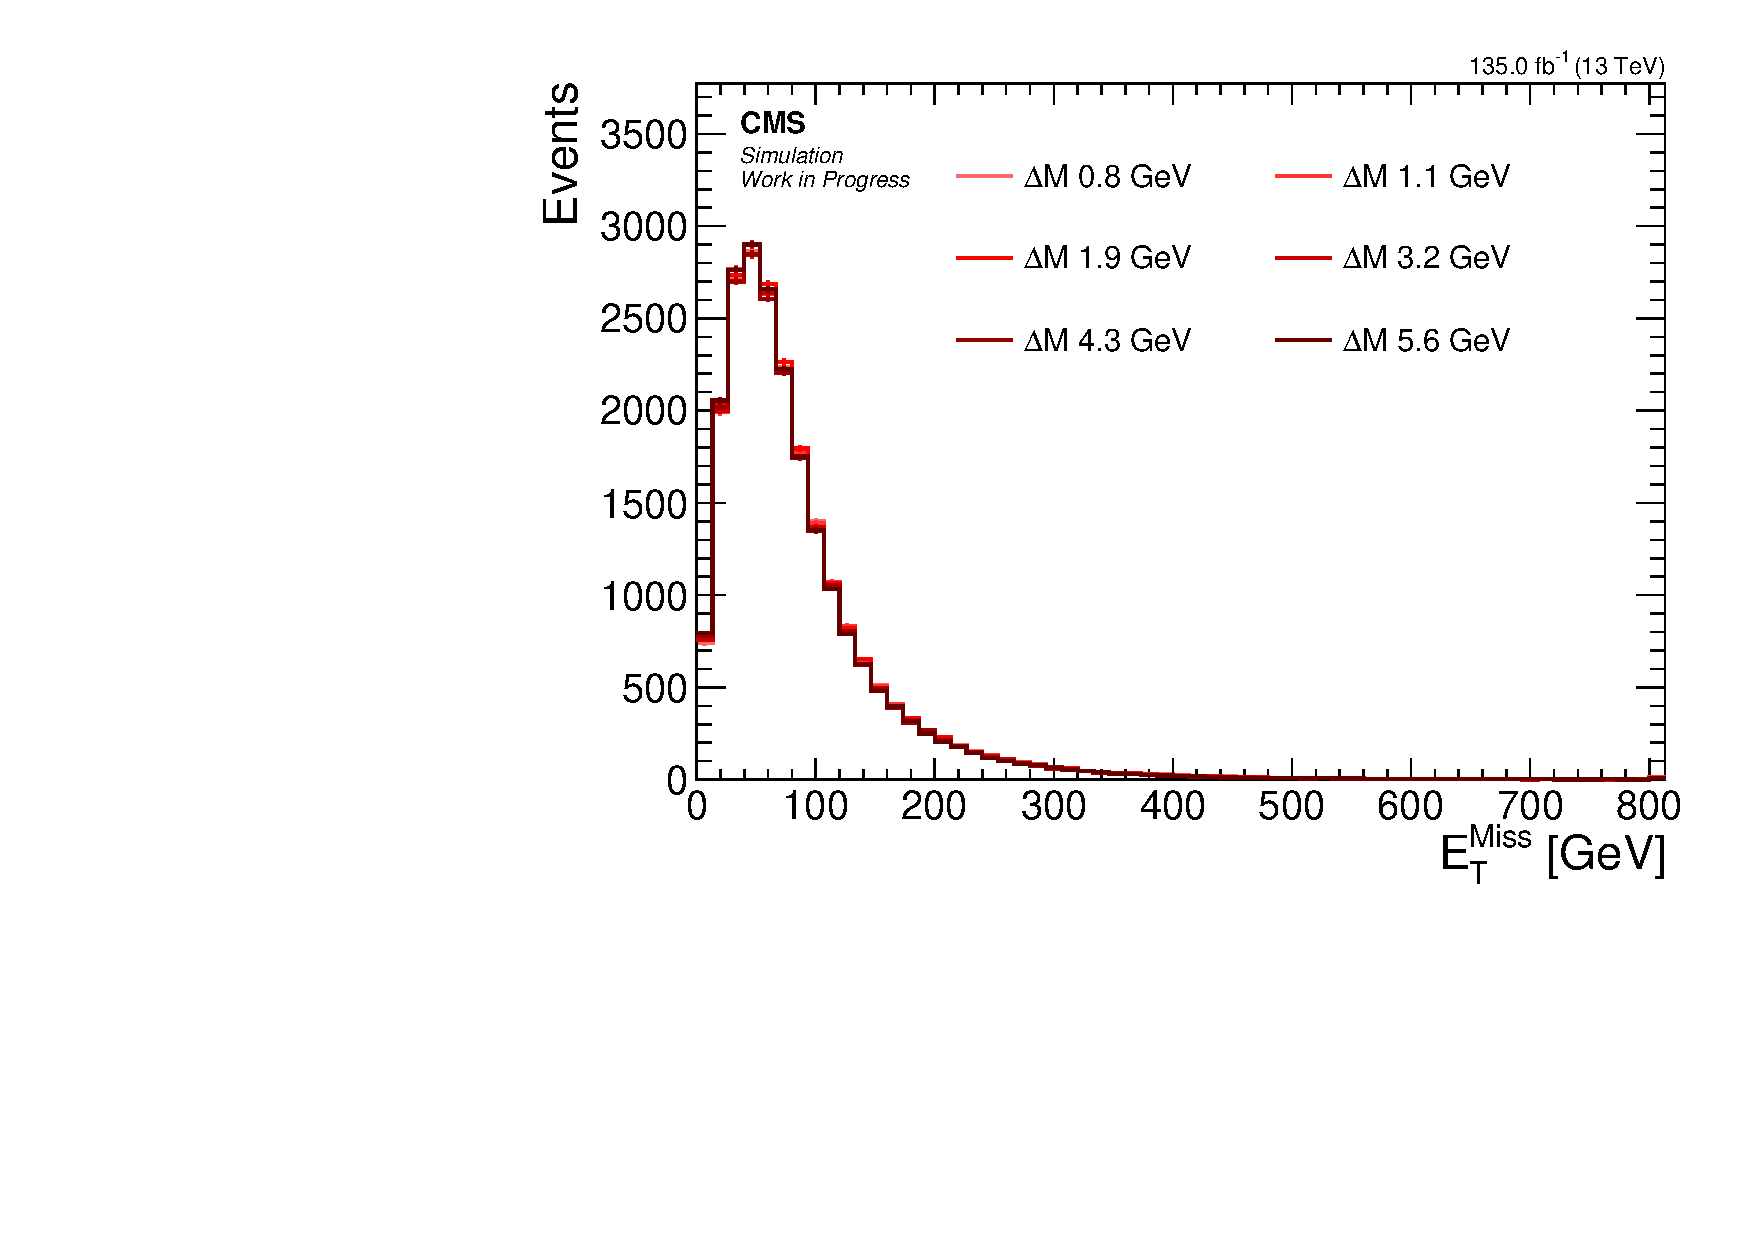
\includegraphics[width=0.48\linewidth]{plots/signal_common_distributions_fixed_mu/none_MET.pdf} \,
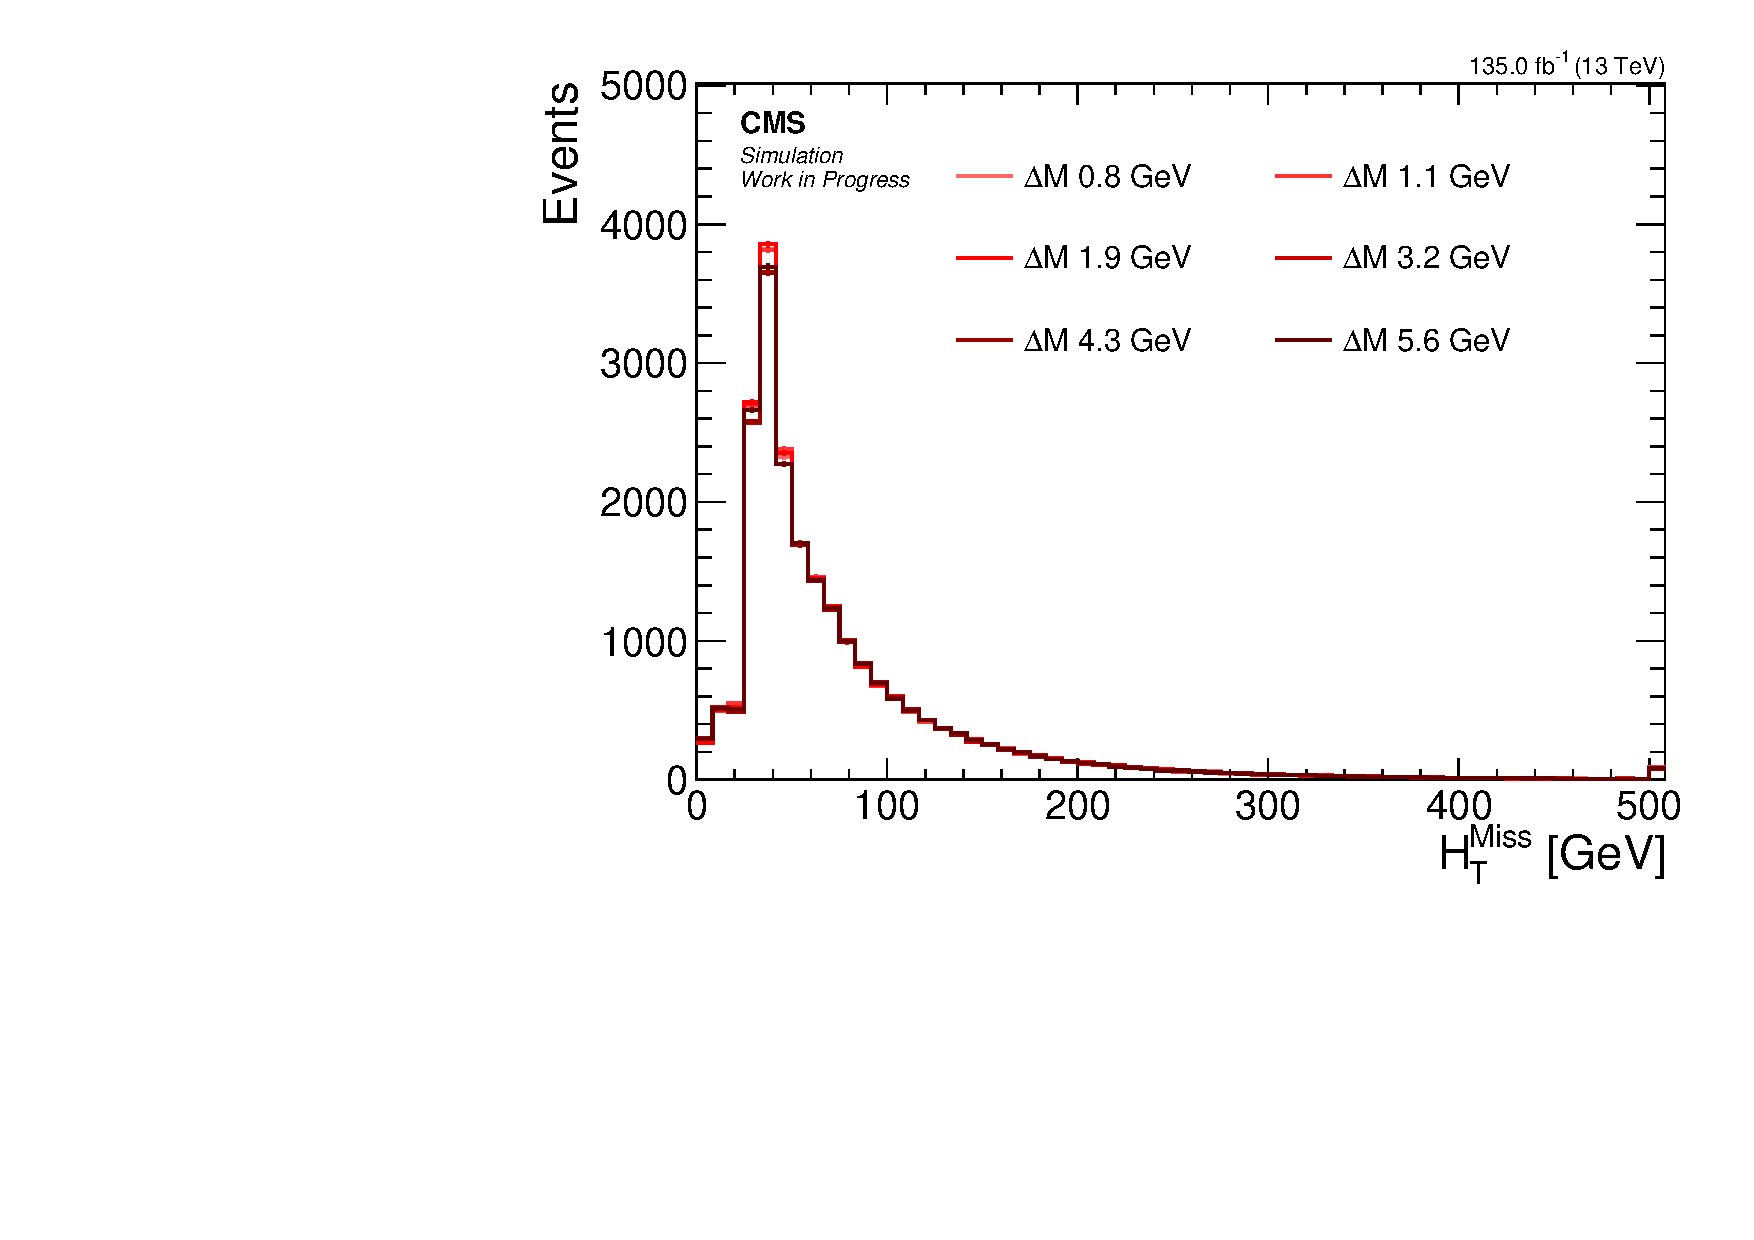
\includegraphics[width=0.48\linewidth]{plots/signal_common_distributions_fixed_mu/none_MHT.pdf}  \\
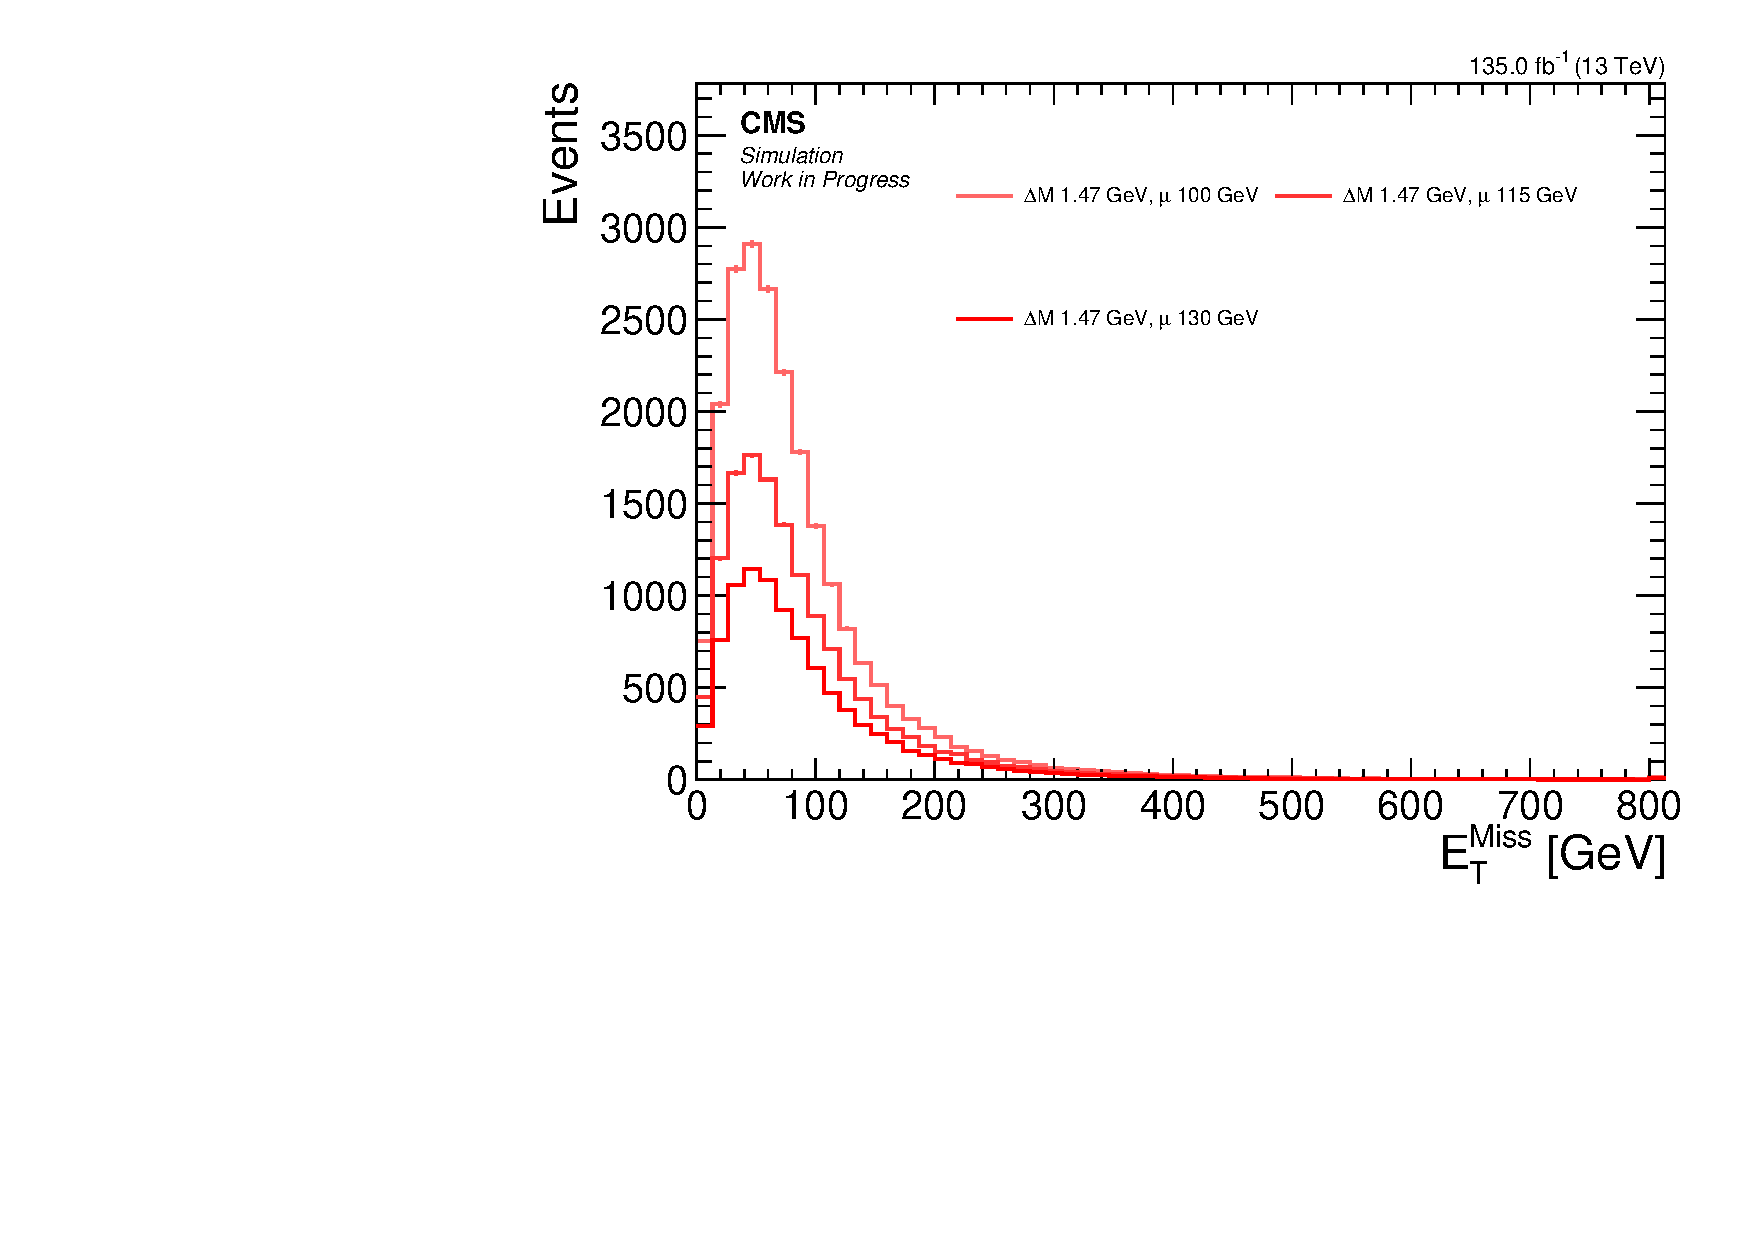
\includegraphics[width=0.48\linewidth]{plots/signal_common_distributions_fixed_dm/none_MET.pdf} \,
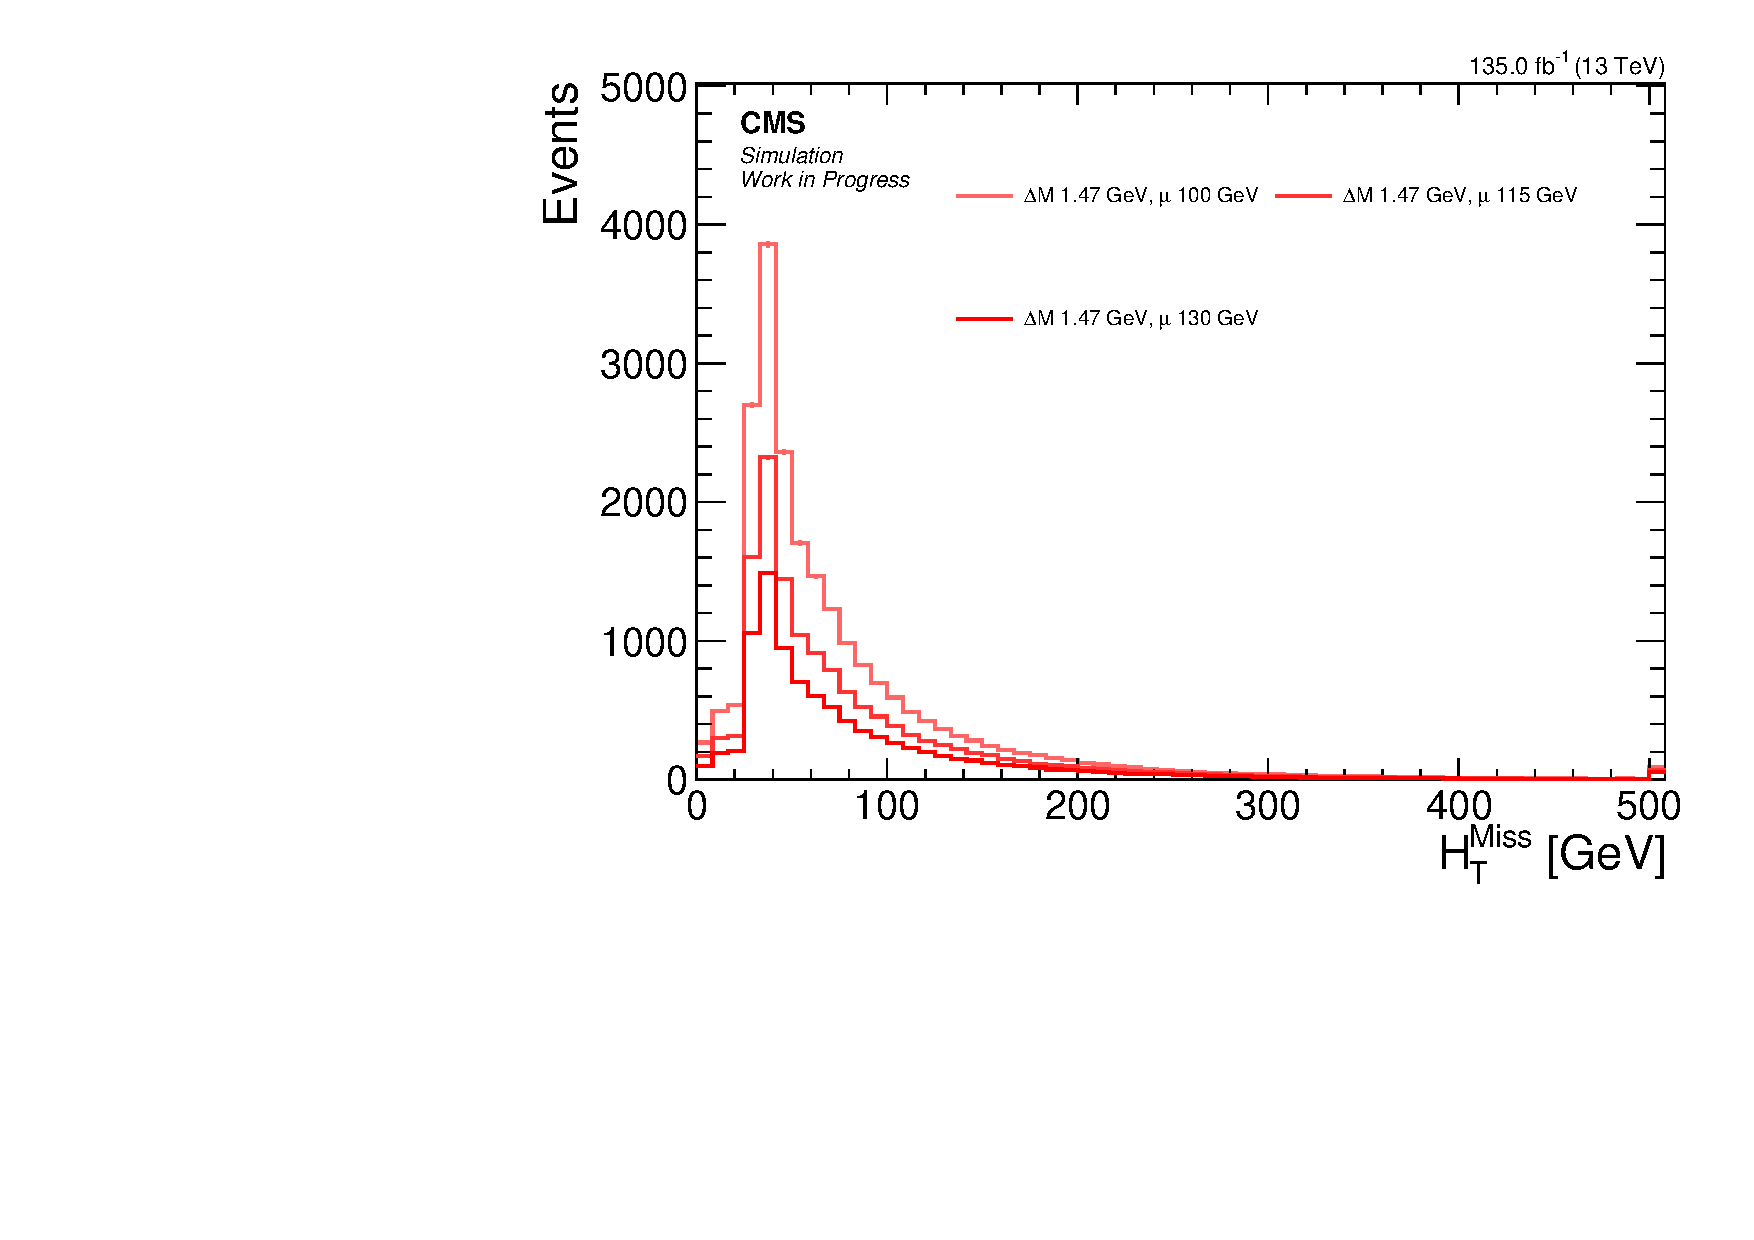
\includegraphics[width=0.48\linewidth]{plots/signal_common_distributions_fixed_dm/none_MHT.pdf}  \\
\caption[Signal $\MET$ and $\mht$ distributions]{ Signal distributions for \MET (left) and \mht (right) comparing various $\dm$ with a fixed higgsino parameter $\mu=100\GeV$ (upper), and comparing various higgsino parameters $\mu$ with fixed $\dm=1.47\GeV$ (lower).}
\label{fig:signal-met-mht}
\end{figure}

As we expect, $\MET$ and $\mht$ are hardly affected by the different choices for \dm, while the higgsino parameter $\mu$ affect the distributions above all through its lower production cross section for higher higgsino parameter $\mu$. As discuss at~\ref{sec:trigger}, the region of interest lie at $\mht\geq 220$ for triggering purposes. Even though this is quite a harsh and inefficient cut, one must look also at the \gls{sm} background at the regions of $\mht < 220$ and $\mht\geq 220$ to conclude that most of the sensitivity comes from the $\mht\geq 220$ region, since the production of real \gls{mht} (or \gls{met}) result from the production of neutrinos in the event, and these are much less common than \gls{qcd} events which swarm the $\mht < 220$ region. Therefore, cutting at $\mht\geq 220$ might be inefficient, but results in high sensitivity. 

\subsection{Jets and hardronic activity}

Since the \glspl{neutralino} \neuto escaping the detector are the contributors to the \gls{mht} and in doing so the drivers of the sensitivity in high \gls{mht} region, we want them to be as boosted as possible, \ie, with the highest transverse momentum \gls{pt} as possible. A widely used approach is to require \fxnote{add citation} an \gls{isr} jet in the event. An \gls{isr} jet is formed when one of the incoming protons emit radiation (such as a photon or a gluon) before the interaction \fxnote{add citation and maybe reference to other section}. If a jet with high enough \gls{pt} is emitted, the rest of the interaction is recoiled against this jet and boosting it in the other direction. This way, the boosted \glspl{neutralino} \neuto will result in higher \gls{mht}. As described in \fxnote{ref}, we require the jets to have $\pt \geq 30\GeV$ and be located within the tracker acceptance $\left(\abs{\eta}<2.4\right)$. We require at least one such jet in the event.
\begin{figure}[!htb]
\centering
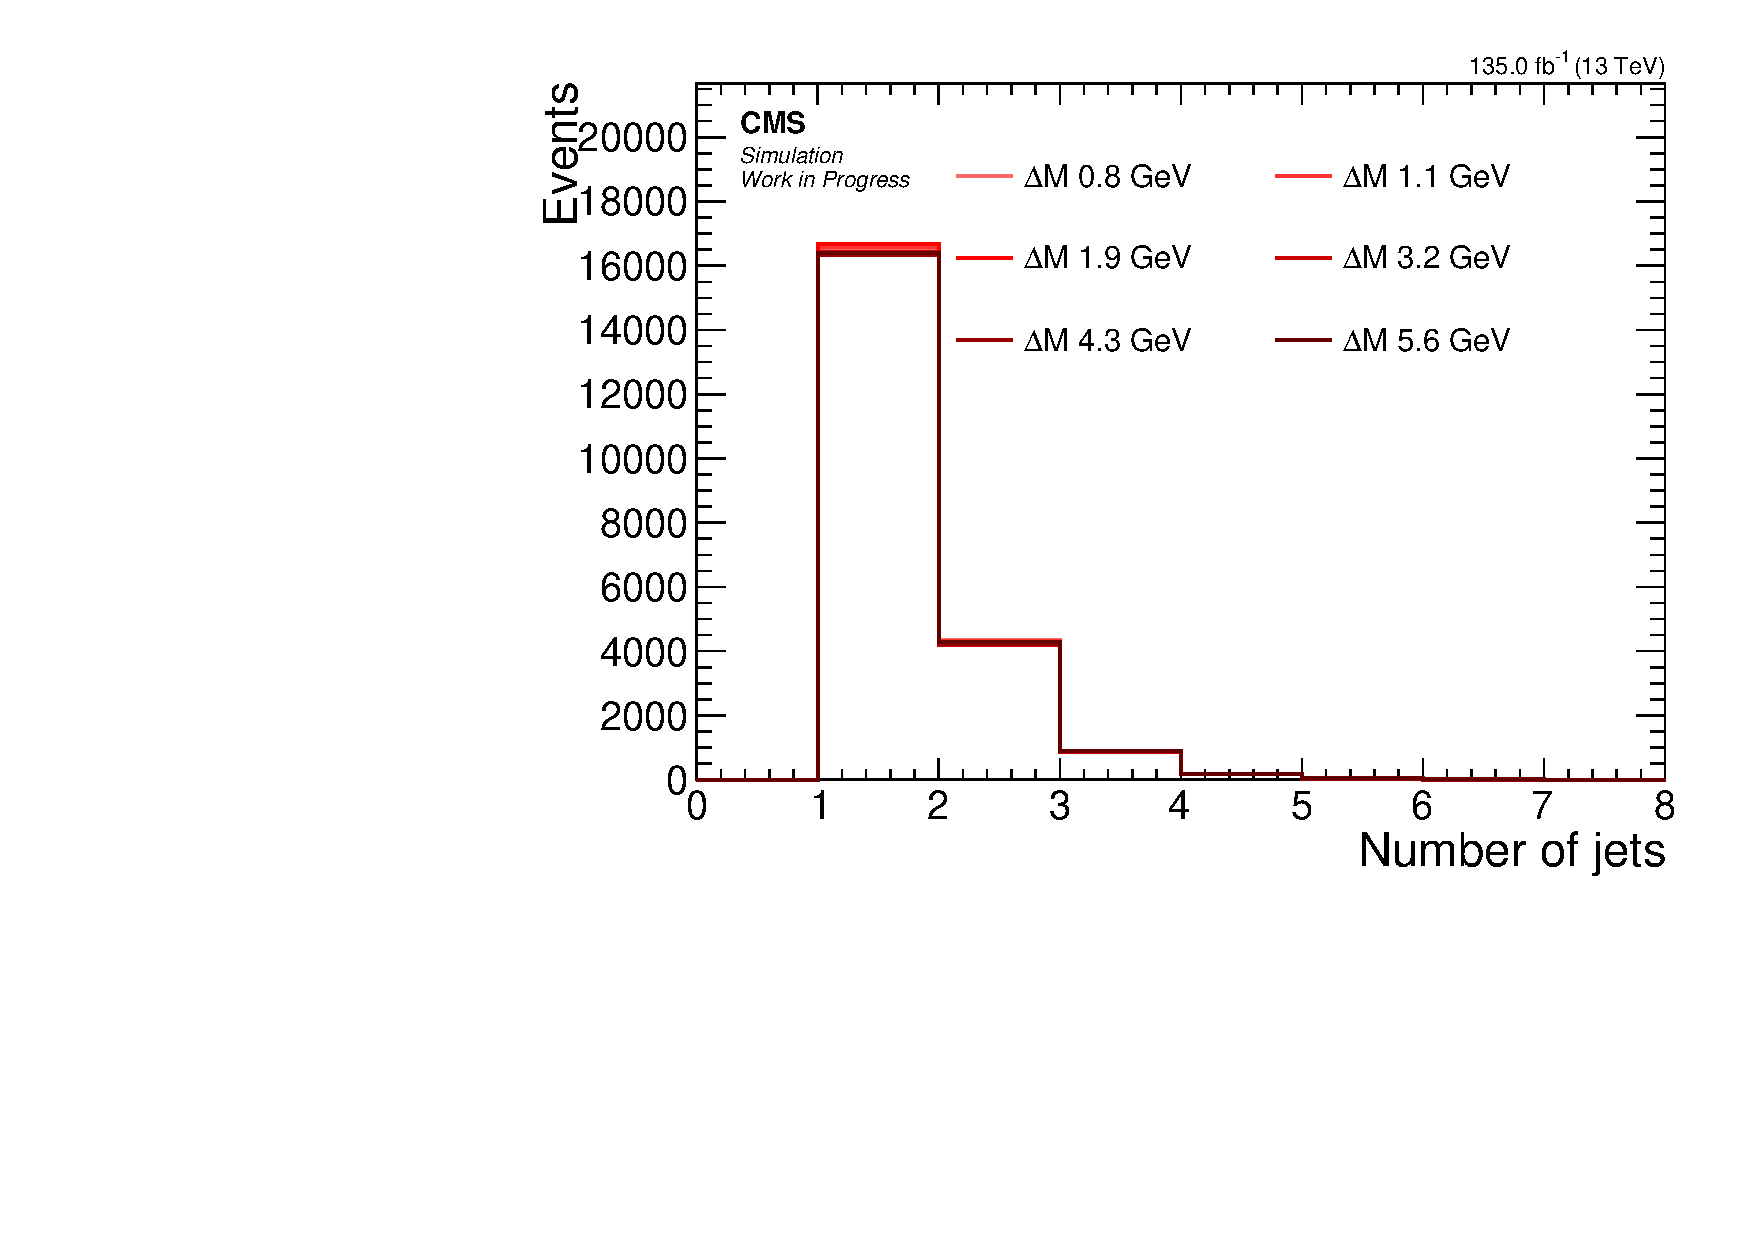
\includegraphics[width=0.48\linewidth]{plots/signal_common_distributions_fixed_mu/none_NJets.pdf} \,
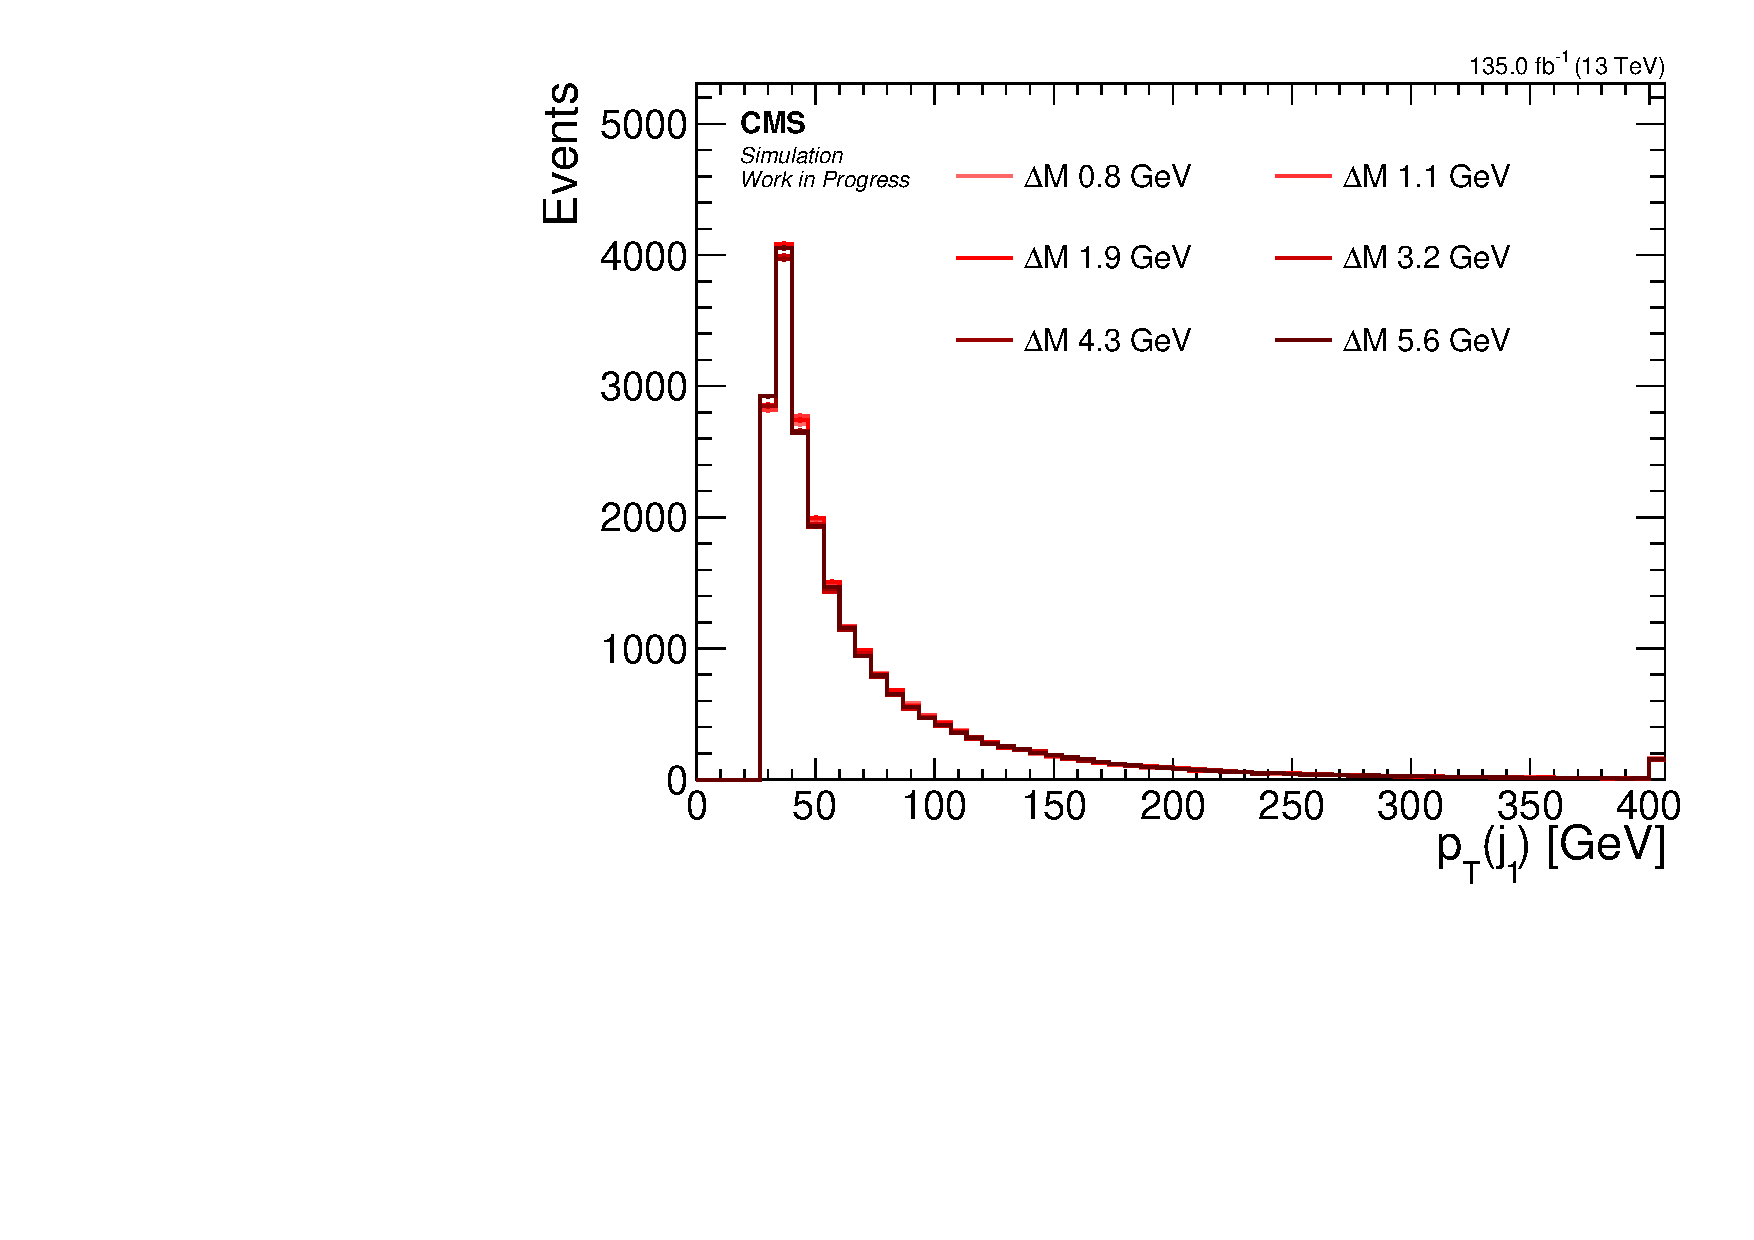
\includegraphics[width=0.48\linewidth]{plots/signal_common_distributions_fixed_mu/none_LeadingJetPt.pdf}  \\
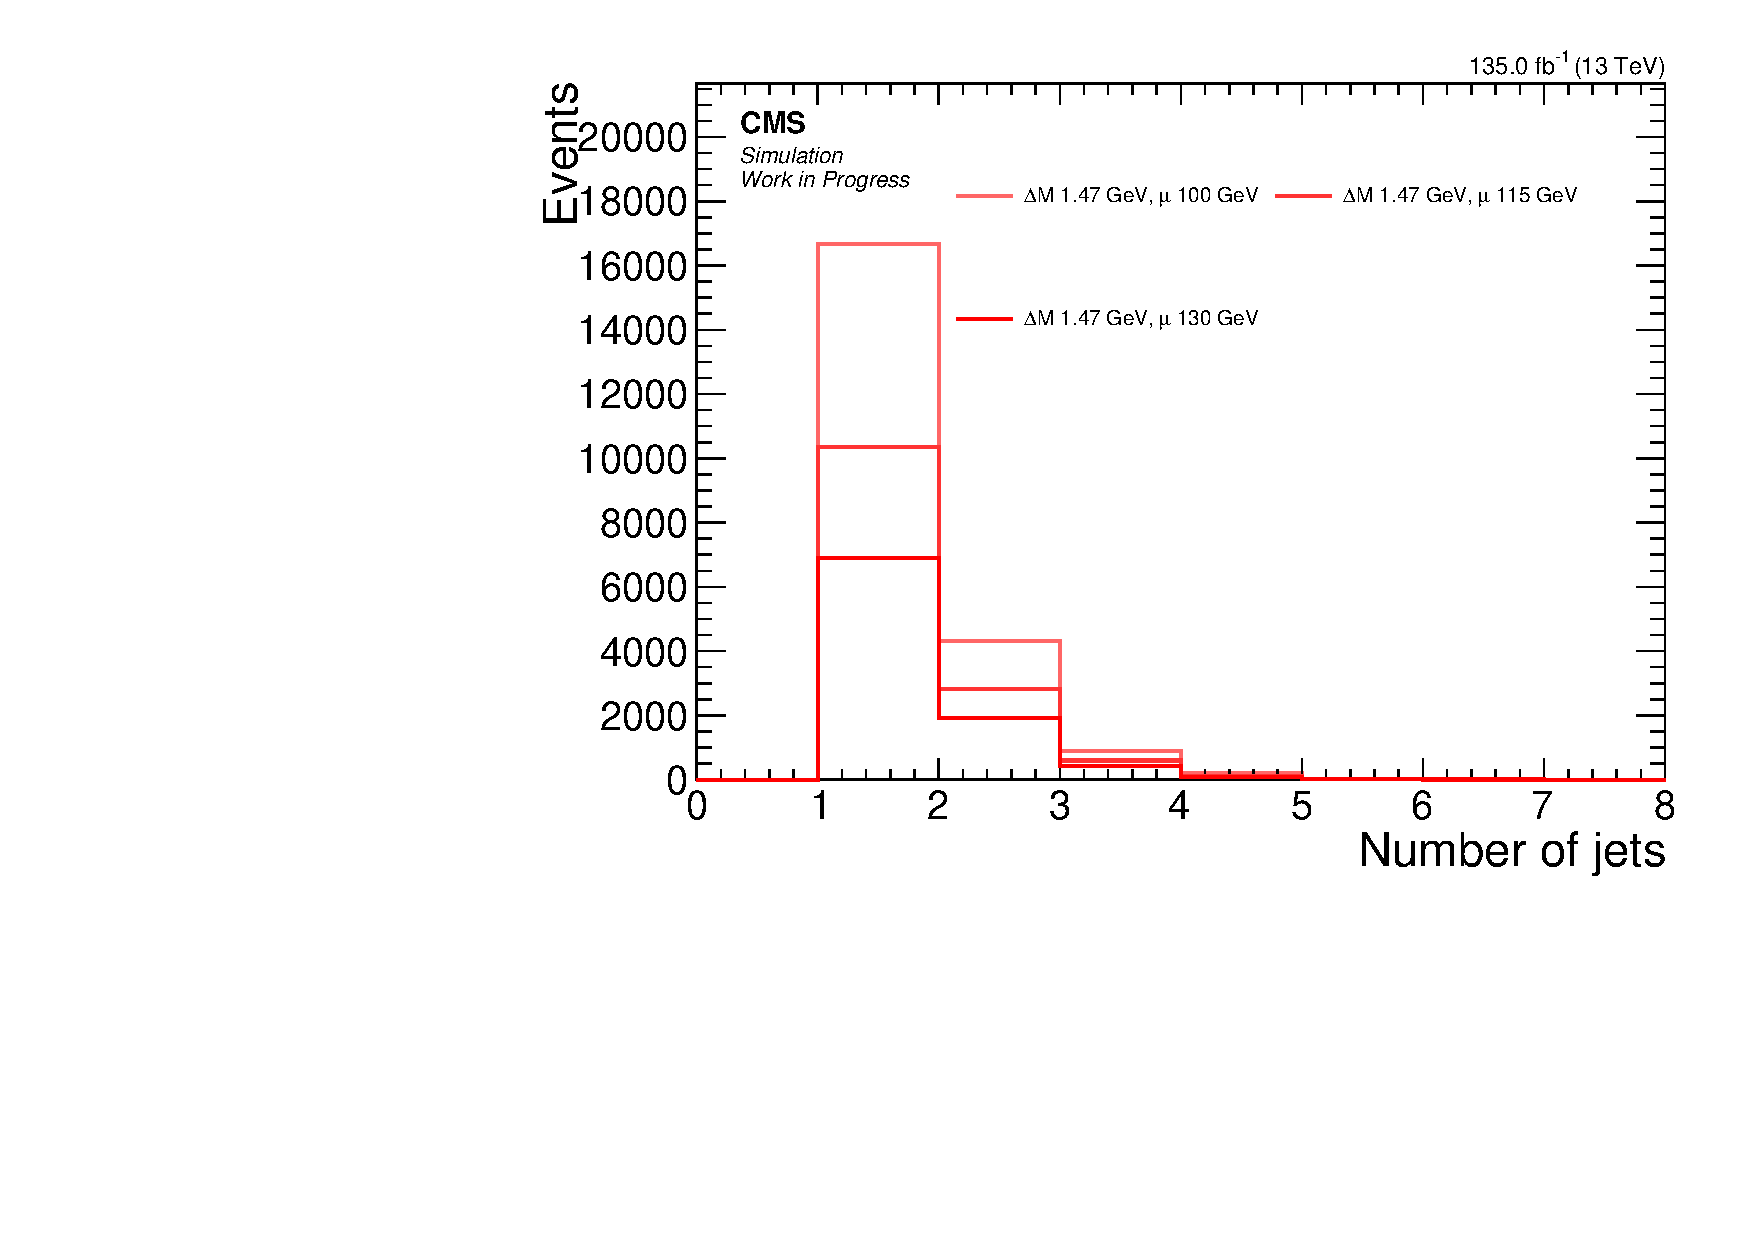
\includegraphics[width=0.48\linewidth]{plots/signal_common_distributions_fixed_dm/none_NJets.pdf} \,
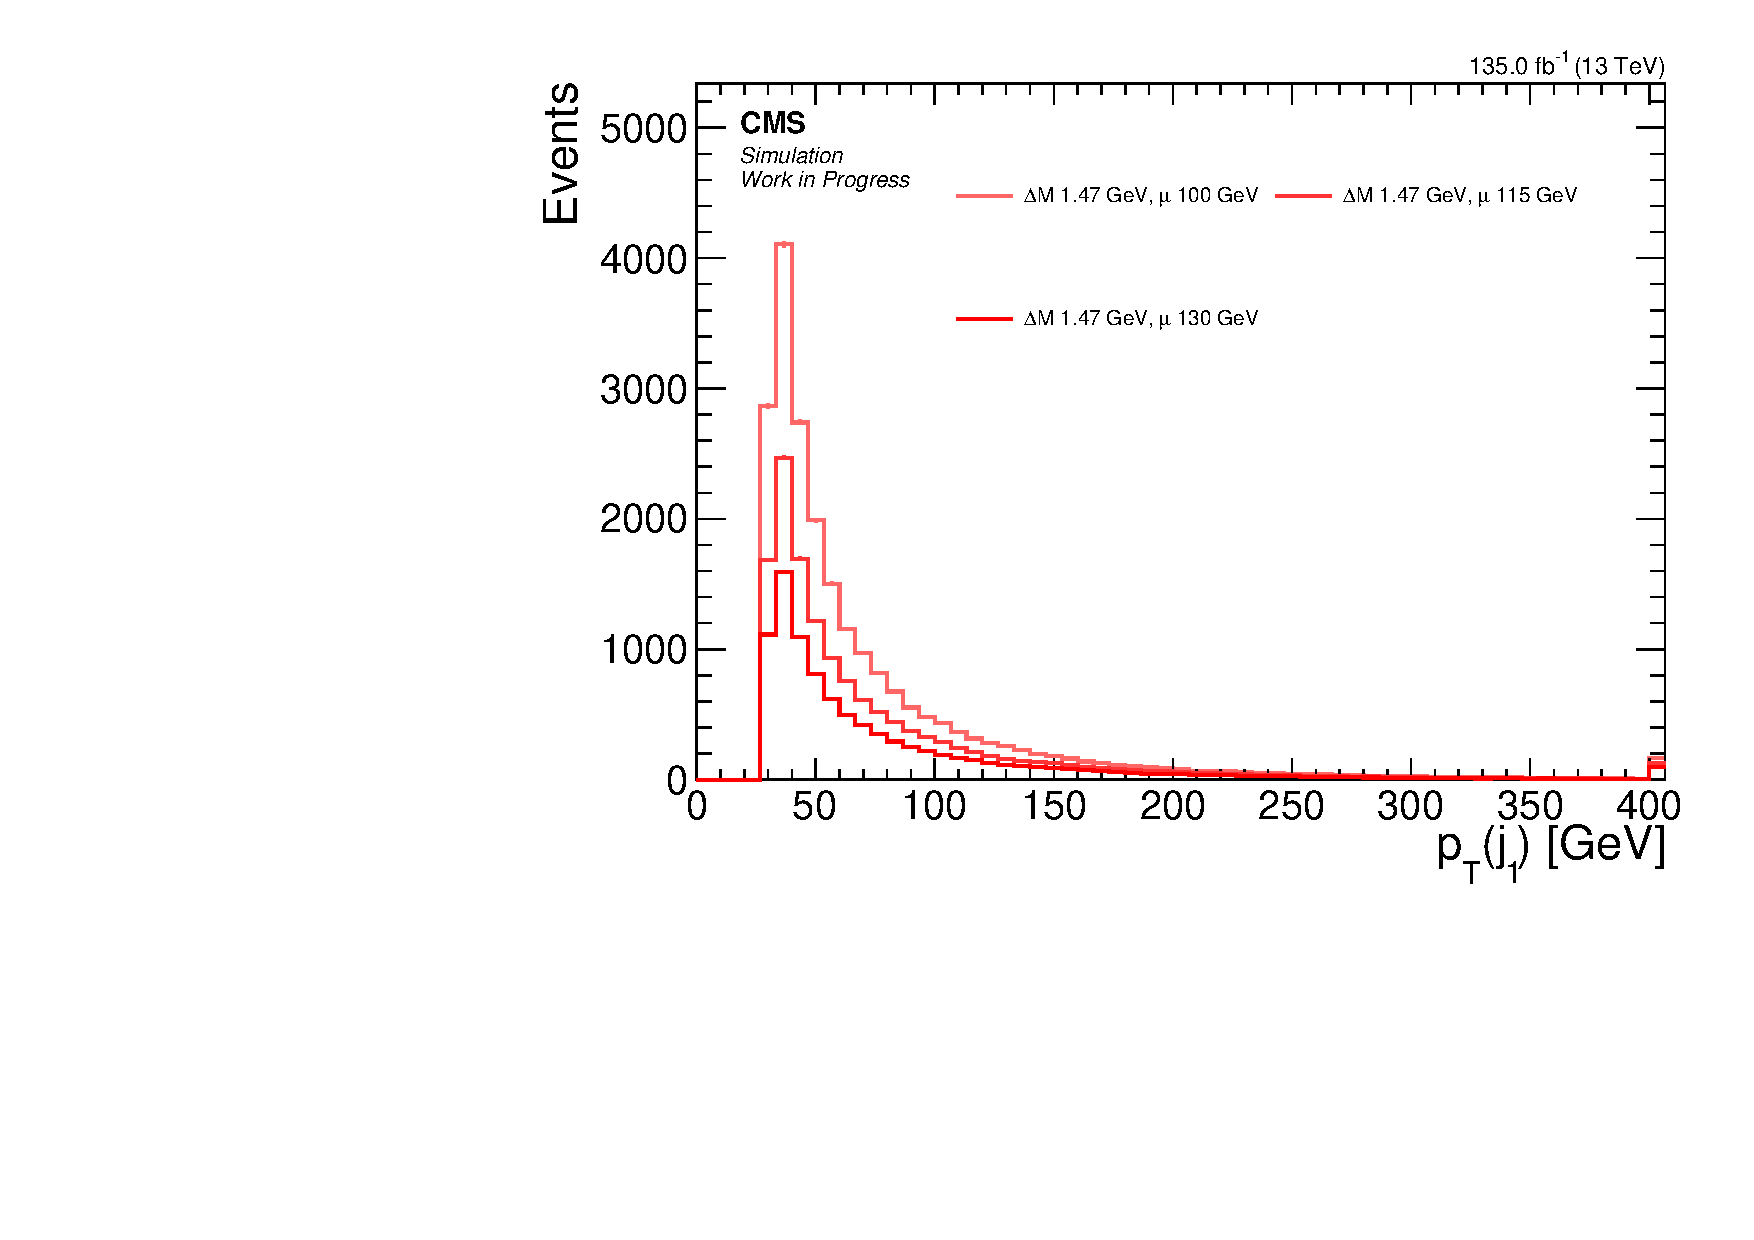
\includegraphics[width=0.48\linewidth]{plots/signal_common_distributions_fixed_dm/none_LeadingJetPt.pdf}  \\
\caption[Signal \emph{number of jets} and \emph{leading jet \pt} distributions]{ Signal distributions for \emph{number of jets} (left) and \emph{leading jet \pt} (right) comparing various $\dm$ with a fixed higgsino parameter $\mu=100\GeV$ (upper), and comparing various higgsino parameters $\mu$ with fixed $\dm=1.47\GeV$ (lower).}
\label{fig:signal-njets-ljpt}
\end{figure}

Our signal signature does not include a \PQb-jet, \ie, a jet resulting from a bottom quark hadronization (either resulting from a top quark or not). We therefore seek to exploit this knowledge by vetoing \PQb-tagged jets in the event. As described in \fxnote{add ref} we are using \DEEPCSV flavor tagging discriminant with a medium working point. As can be seen in these distributions, most of the signal lie in the 0 bin, and we will therefore veto any \PQb-tagged jet, which retains most of the signal, but rejects a lot of \gls{sm} background, such as arising from \ttbar events. 

\begin{figure}[!htb]
\centering
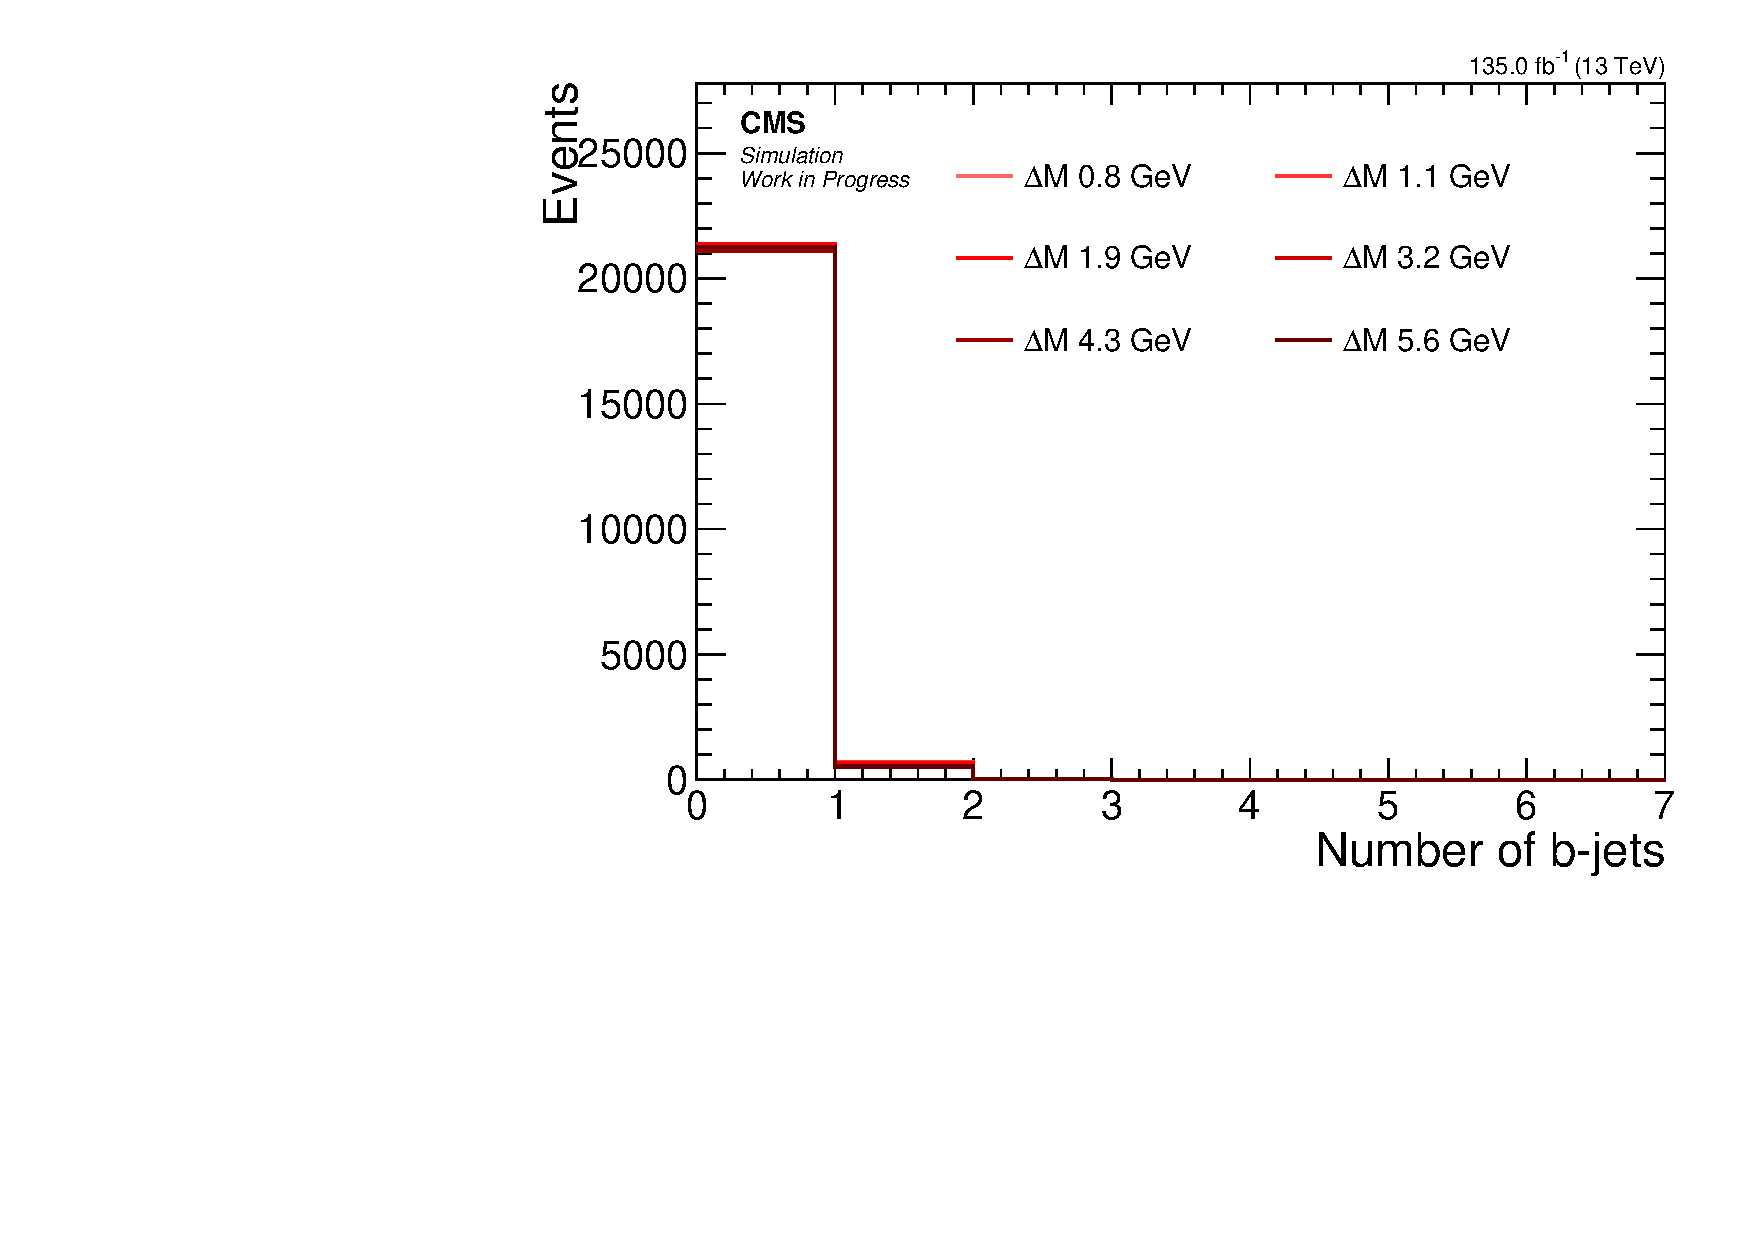
\includegraphics[width=0.48\linewidth]{plots/signal_common_distributions_fixed_mu/none_BTagsDeepMedium.pdf} \,
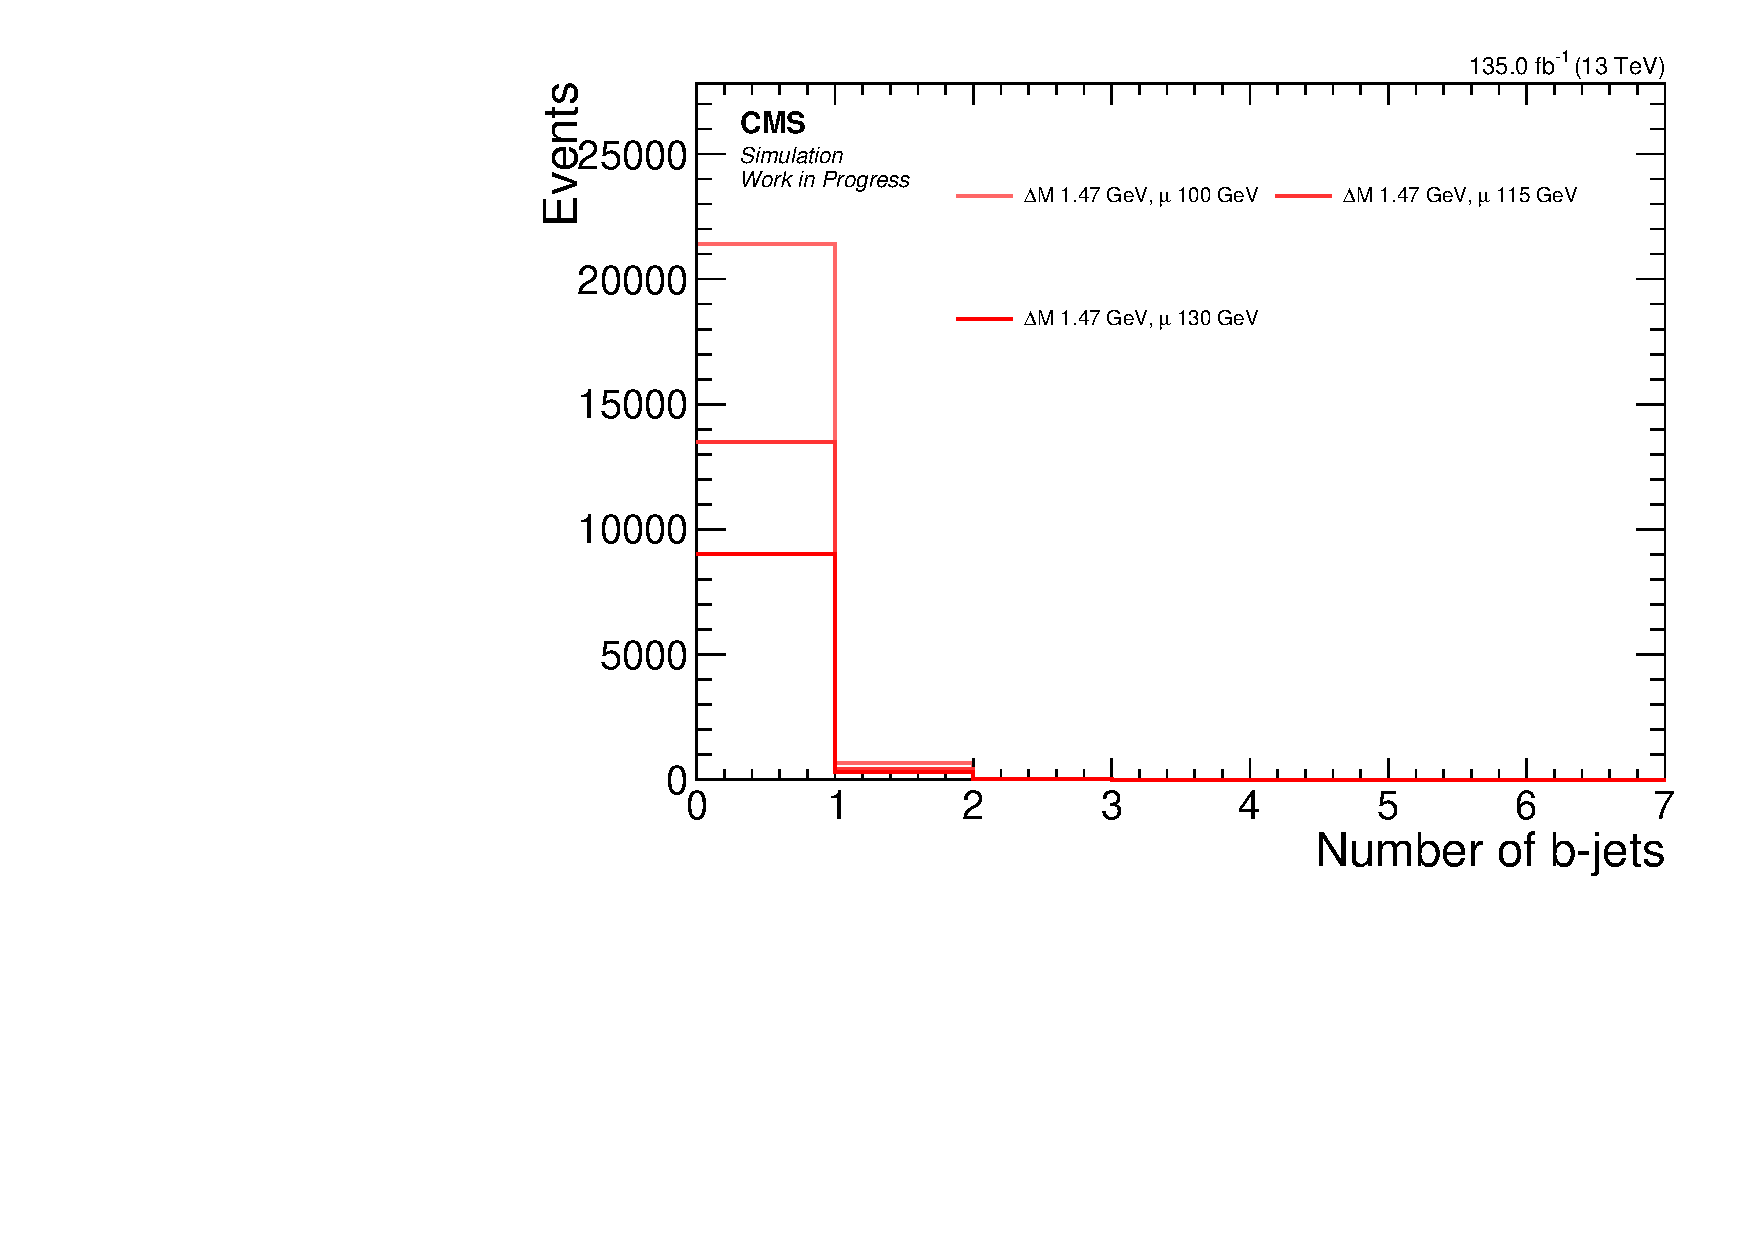
\includegraphics[width=0.48\linewidth]{plots/signal_common_distributions_fixed_dm/none_BTagsDeepMedium.pdf}  \\
\caption[Signal \emph{number of b-tagged jets} distributions]{ Signal distributions for \emph{number of b-tagged jets} comparing various $\dm$ with a fixed higgsino parameter $\mu=100\GeV$ (left), and comparing various higgsino parameters $\mu$ with fixed $\dm=1.47\GeV$ (right).}
\label{fig:signal-bjets}
\end{figure}

Since we are requiring an \gls{isr} jet in the event, we expect the \gls{met} and the \gls{mht} to point in the opposite direction of the jet, or at least in an angel close to $\pi$. Events with multiple jets in the \gls{sm} background such as arising from \gls{qcd} will not exhibit such a feature. In order to reduce \gls{qcd} background, we require $\mindphimhtjets > 0.4$.

\begin{figure}[!htb]
\centering
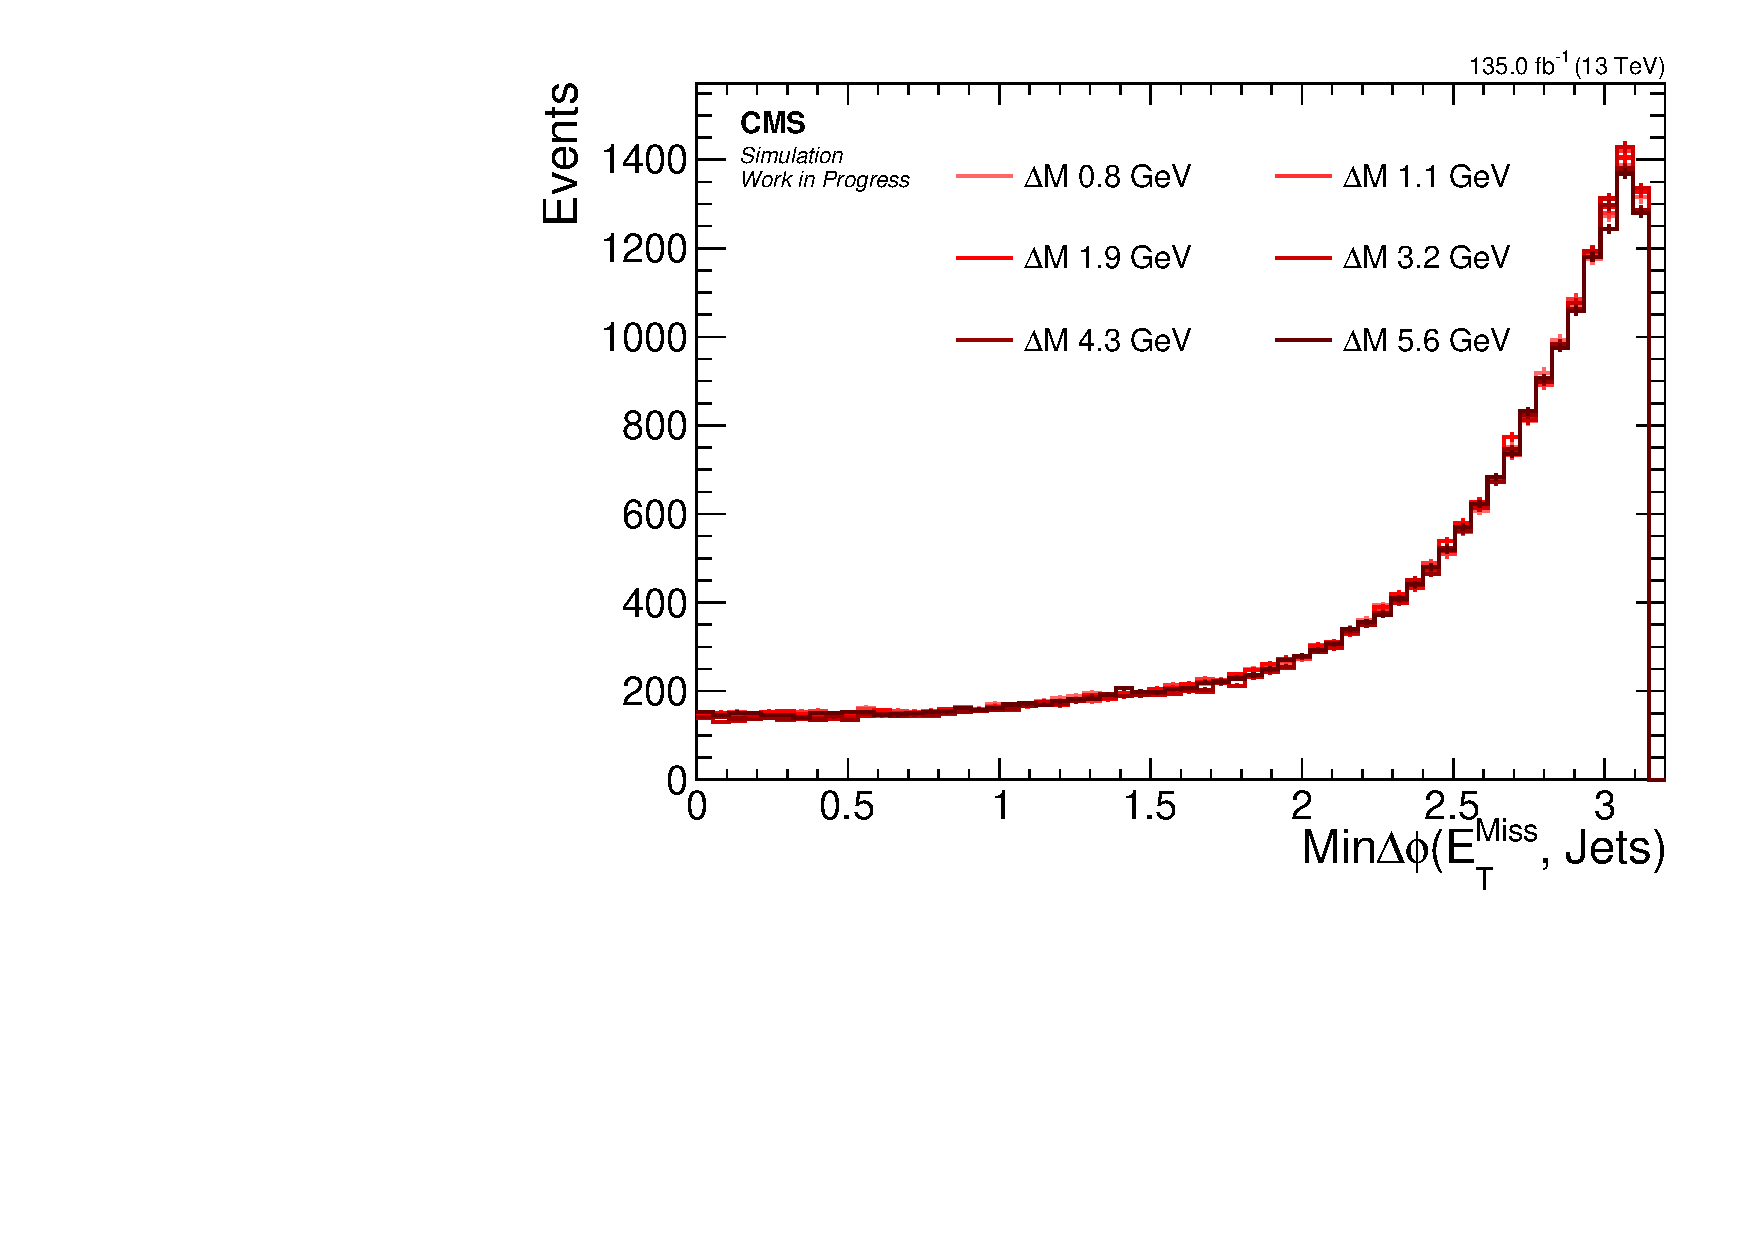
\includegraphics[width=0.48\linewidth]{plots/signal_common_distributions_fixed_mu/none_MinDeltaPhiMetJets.pdf} \,
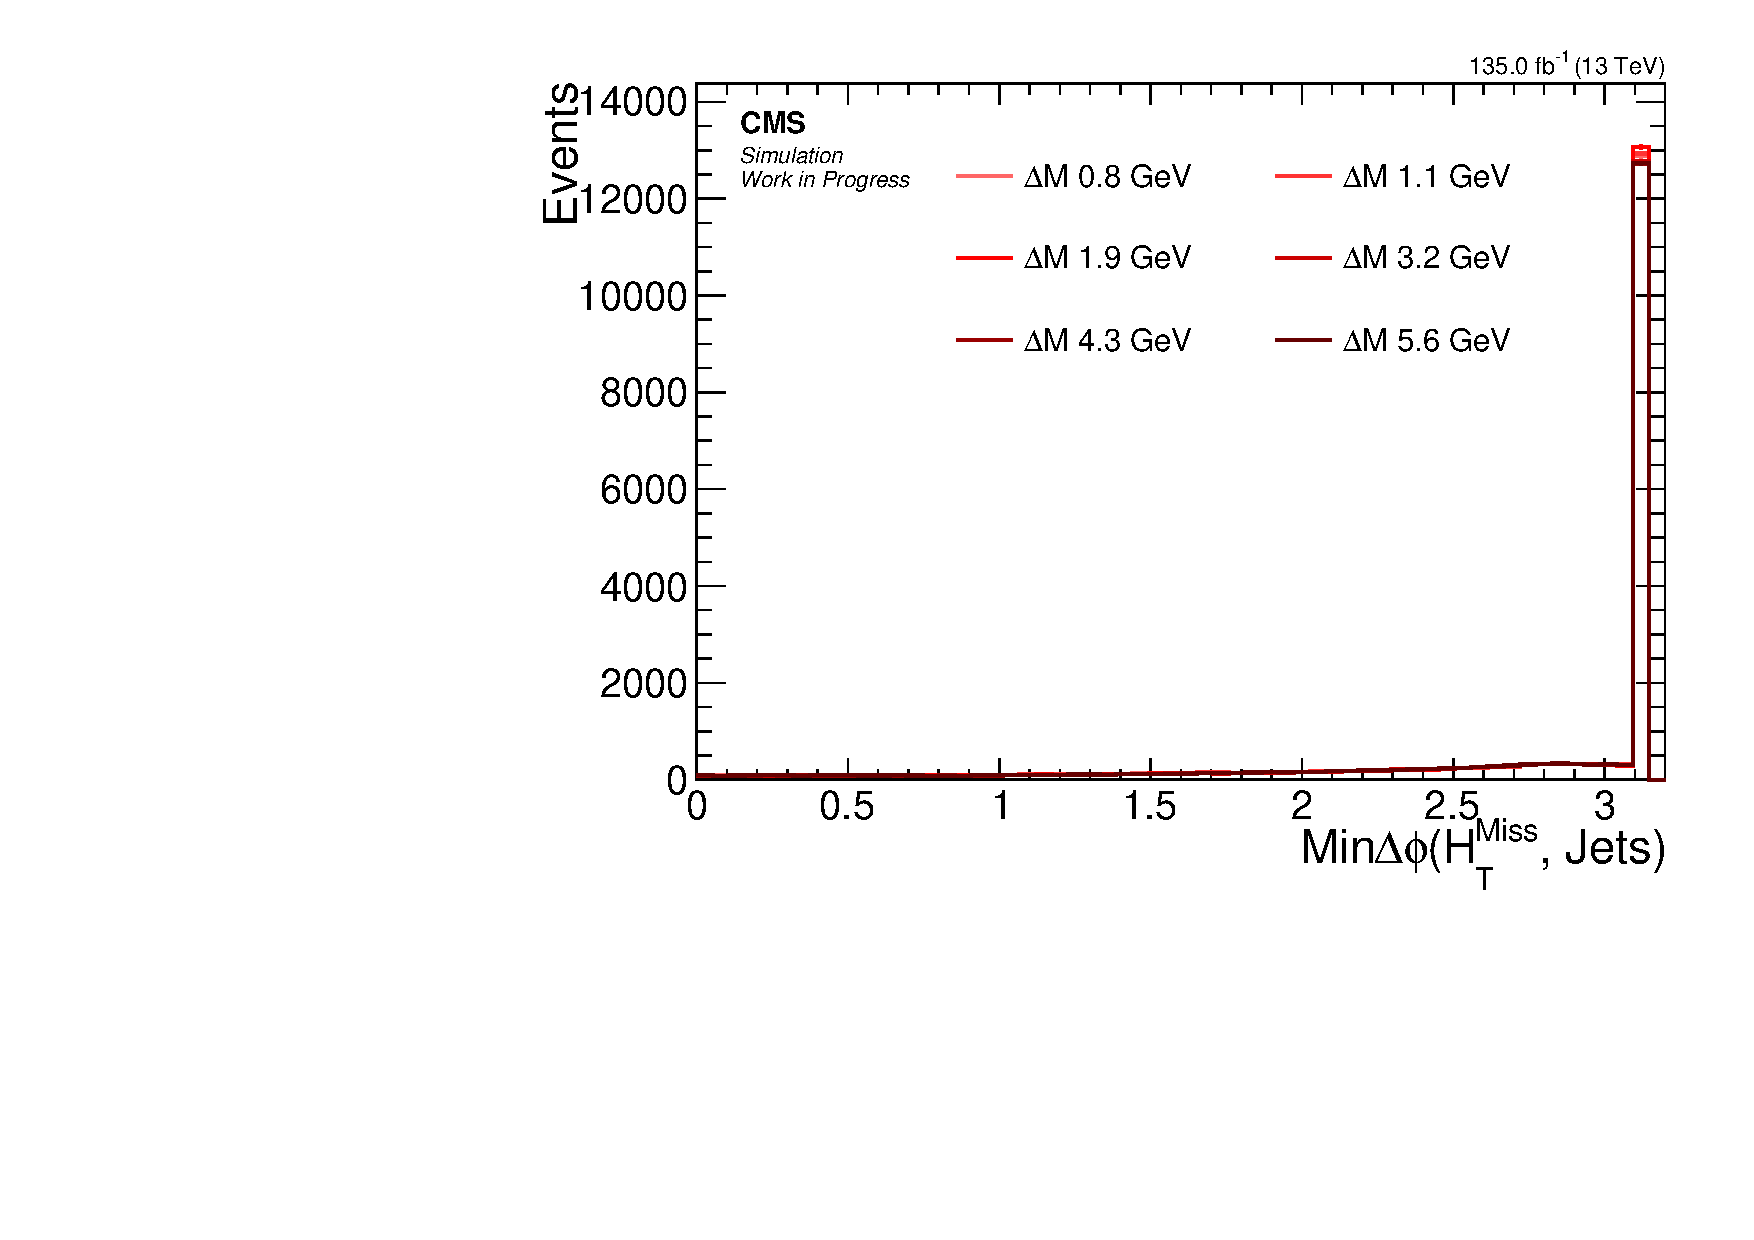
\includegraphics[width=0.48\linewidth]{plots/signal_common_distributions_fixed_mu/none_MinDeltaPhiMhtJets.pdf}  \\
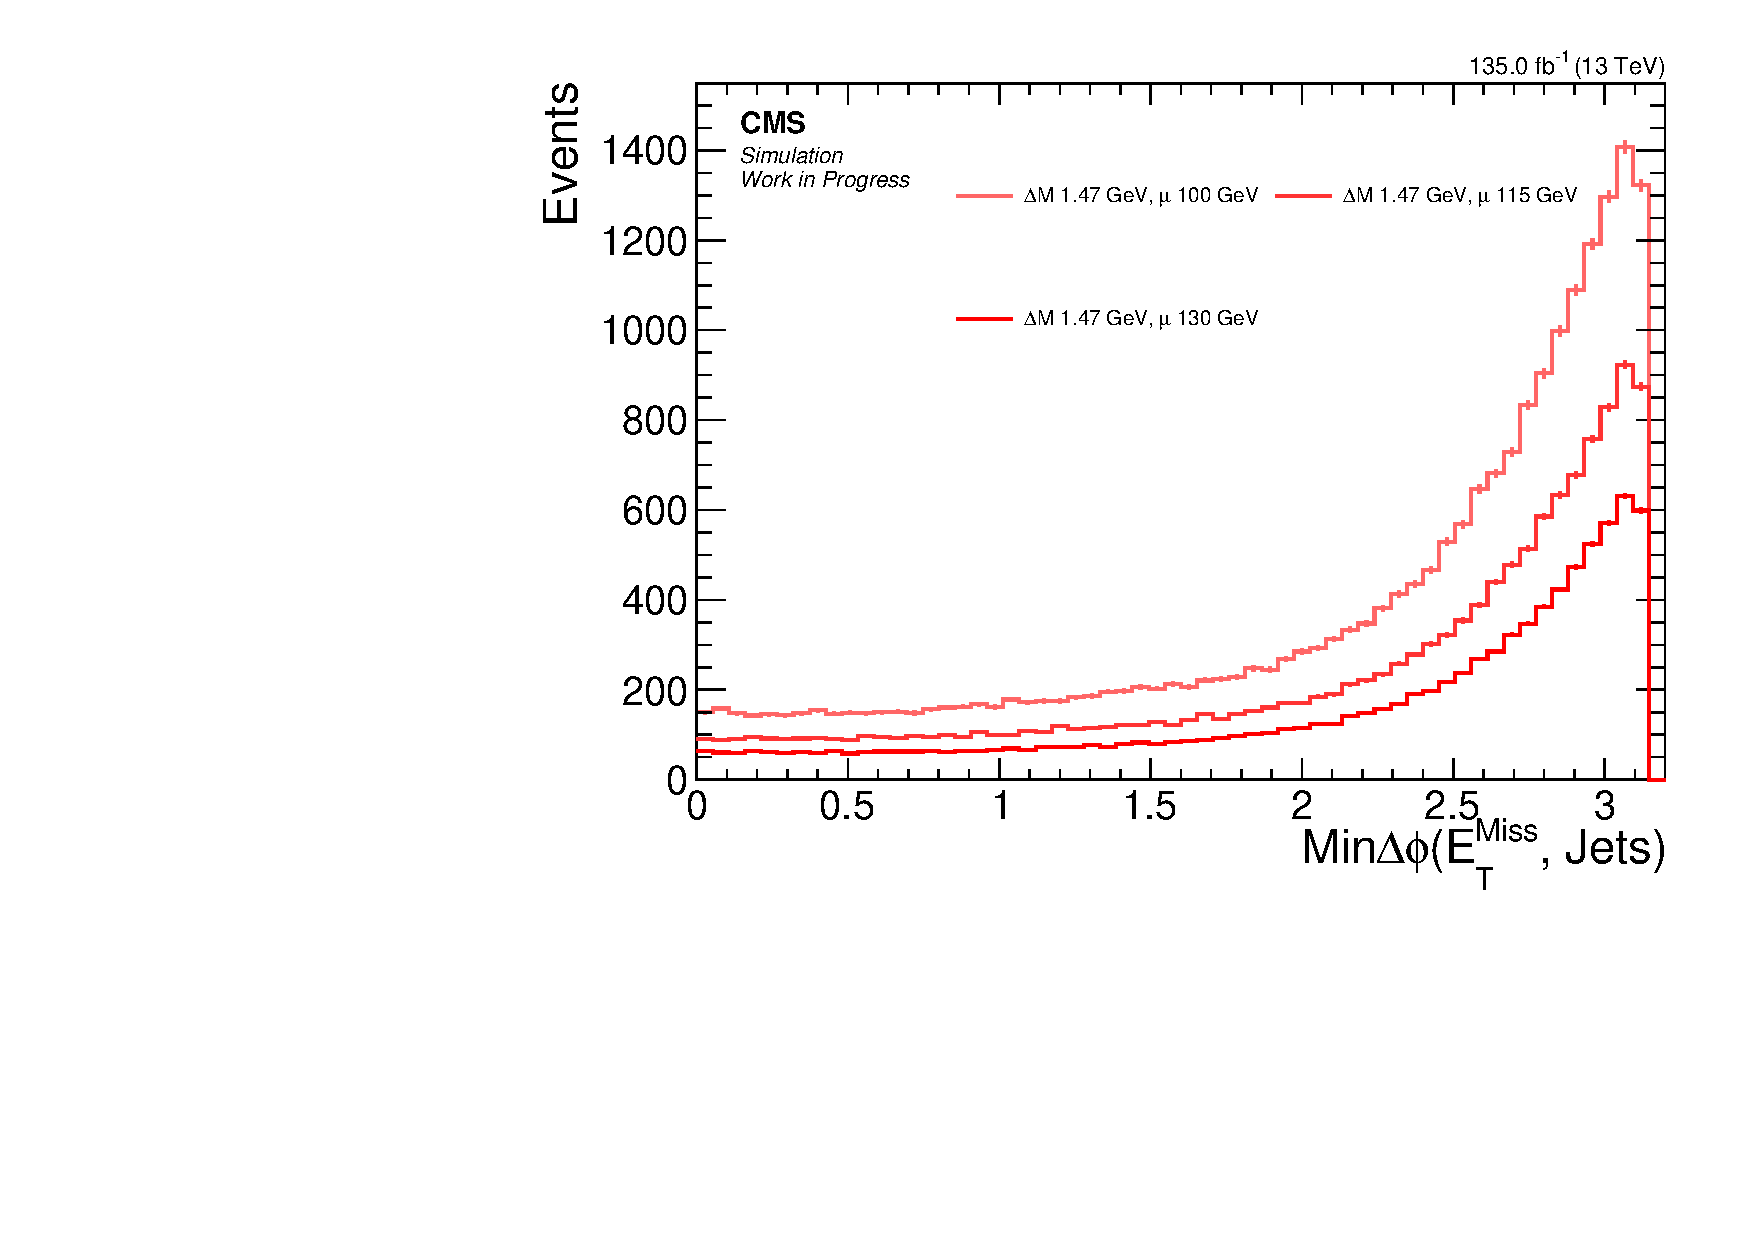
\includegraphics[width=0.48\linewidth]{plots/signal_common_distributions_fixed_dm/none_MinDeltaPhiMetJets.pdf} \,
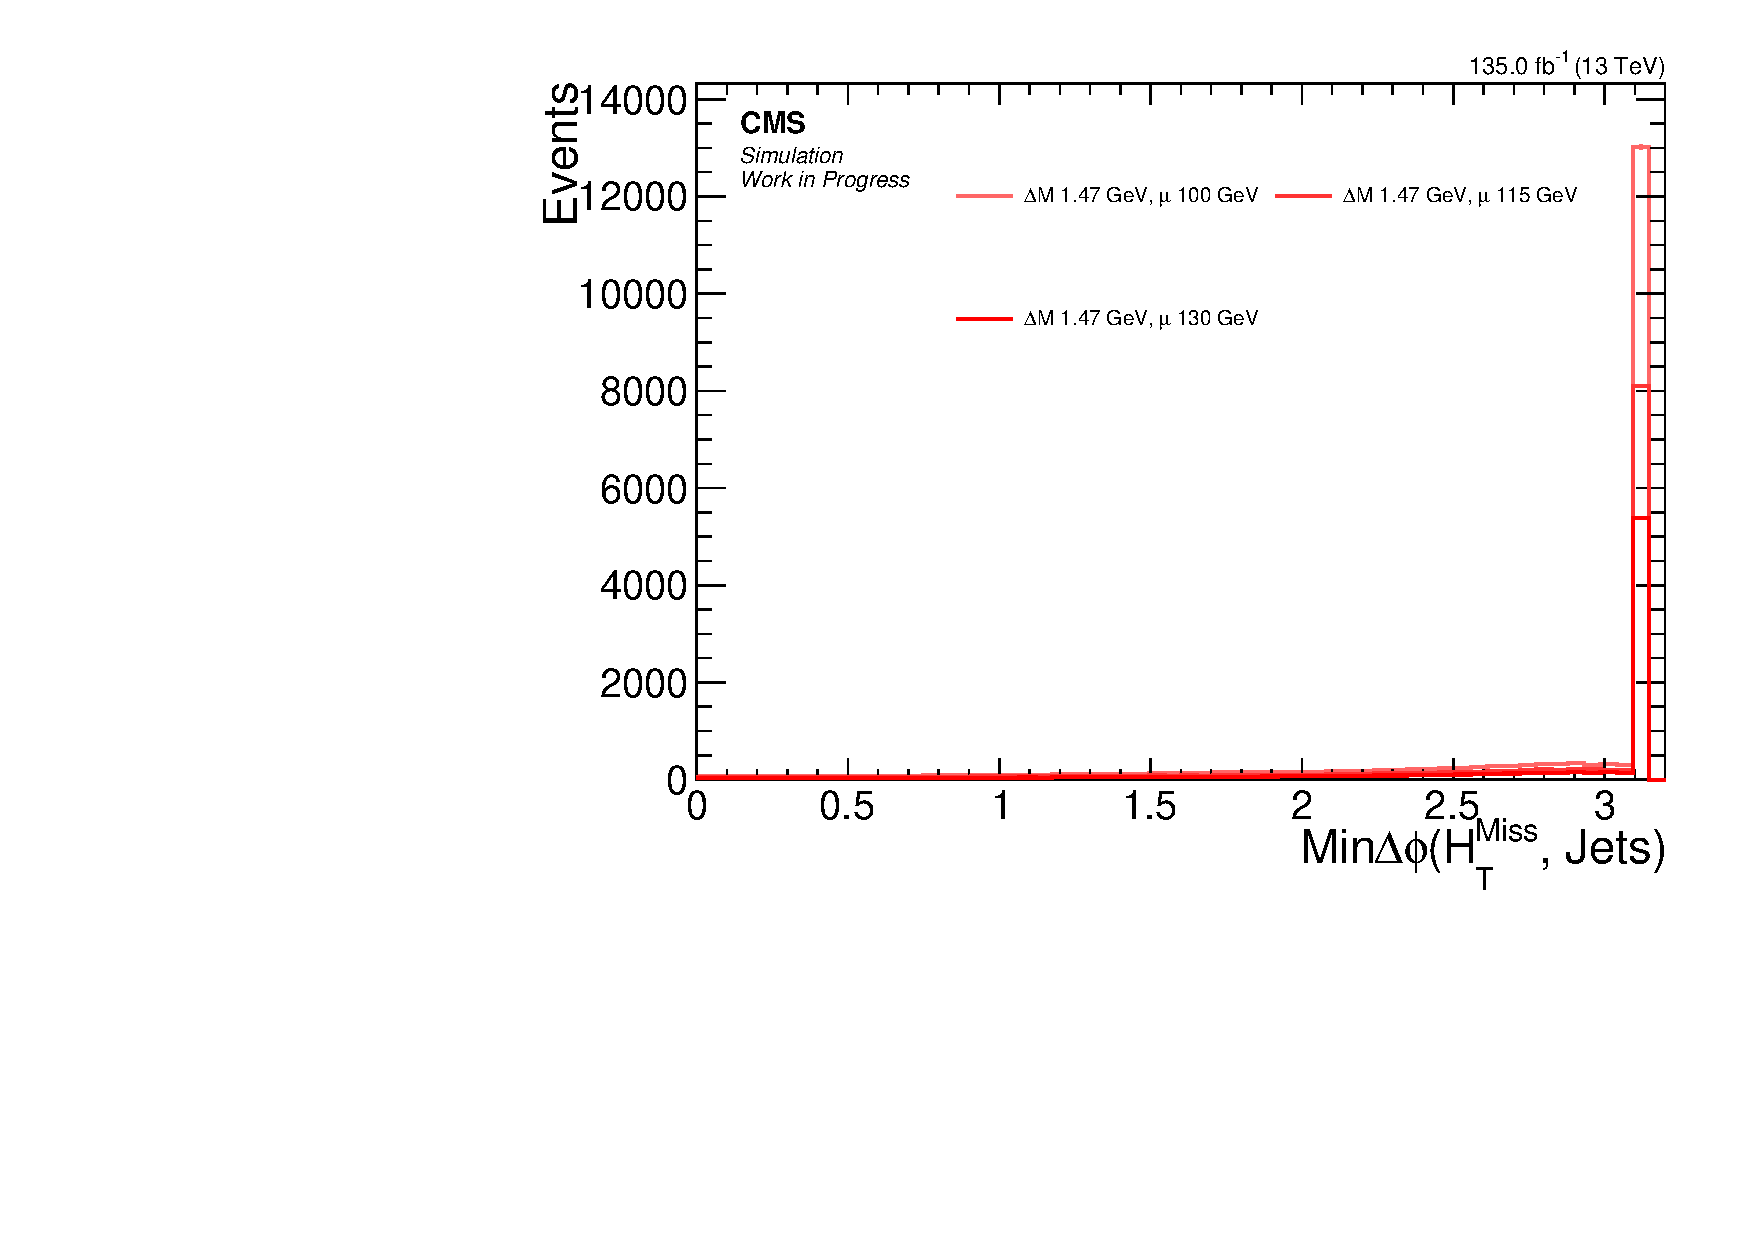
\includegraphics[width=0.48\linewidth]{plots/signal_common_distributions_fixed_dm/none_MinDeltaPhiMhtJets.pdf}  \\
\caption[Signal $\mindphimetjets$ and $\mindphimhtjets$ distributions]{ Signal distributions for \mindphimetjets (left) and \mindphimhtjets (right) comparing various $\dm$ with a fixed higgsino parameter $\mu=100\GeV$ (upper), and comparing various higgsino parameters $\mu$ with fixed $\dm=1.47\GeV$ (lower).}
\label{fig:signal-min-deltaphi-met-mht}
\end{figure}

\subsection{Base selection}

We recap the section by summarizing the base selection of our analysis. This base selection, or preselection as we might use call it interchangeably, is applied to all analysis categories. 

\begin{table}[!htb]
	\centering
	\label{tab:base-selection}
		\caption{Base selection applied to all analysis categories}
		%\vspace{1mm}
			\begin{tabular}{lc} \hline
			Variable & Value \\ \hline
			$\mht \left[\GeV\right]$ & $\geq220$ \\
			$\njets \left( \pt \geq 30\GeV\, \mathrm{and}\, \abs{\eta} < 2.4 \right)$ & $\geq 1$\\
			$\nbjets \left( \pt \geq 30\GeV\, \mathrm{and}\, \abs{\eta} < 2.4 \right)$ & 0 \\
			$\mindphimhtjets$ & $ > 0.4$ \\ \hline
			\end{tabular}
\end{table}

\subsection{Dilepton kinematics}

Thus far we have looked at kinematic distributions ignoring the leptons in event. However, the most distinct features of the signal lie in the dilepton system. To fully understand the unique phase space of the dilepton system, we first look at generator level distributions and then look at what effects does reconstruction have on those observables. In addition, since the most sensitive category is the dimuon category due to its much lower threshold on the transverse momentum, these events are shown in the following sections, leaving the events with two electrons to the appendix \fxnote{ref}.

Since the kinematics changes dramatically as a function of \dm, but changes almost only in overall normalization due to the production cross section as a function of the higgsino parameter $\mu$, in the following sections, we set the higgsino parameter to $\mu=100\GeV$ and vary the \dm.

\subsubsection{Lepton $\eta$ and transverse momentum \gls{pt}}
\label{sec:muon-eta-pt}

The transverse momentum \gls{pt} distribution of the muons and our access to a subset of its full range, have dramatic effect on the signal acceptance and the sensitivity. The muon reconstruction process and details are discussed in \fxnote{ref}. The selection we apply to the muons in this analysis is described in~\ref{sec:muon-selection} and will be referred to here as \emph{analysis selection}. In this section we would like to consider specifically the importance of the \gls{pt} on the signal and its dilepton kinematic distributions.

We begin by having a look at the generator level distribution of \gls{pt}, or in other words, the so-called \emph{truth} distributions, which do not exhibit any detector or reconstruction features, and compare to the reconstructed distribution.

\begin{figure}[!htb]
\centering
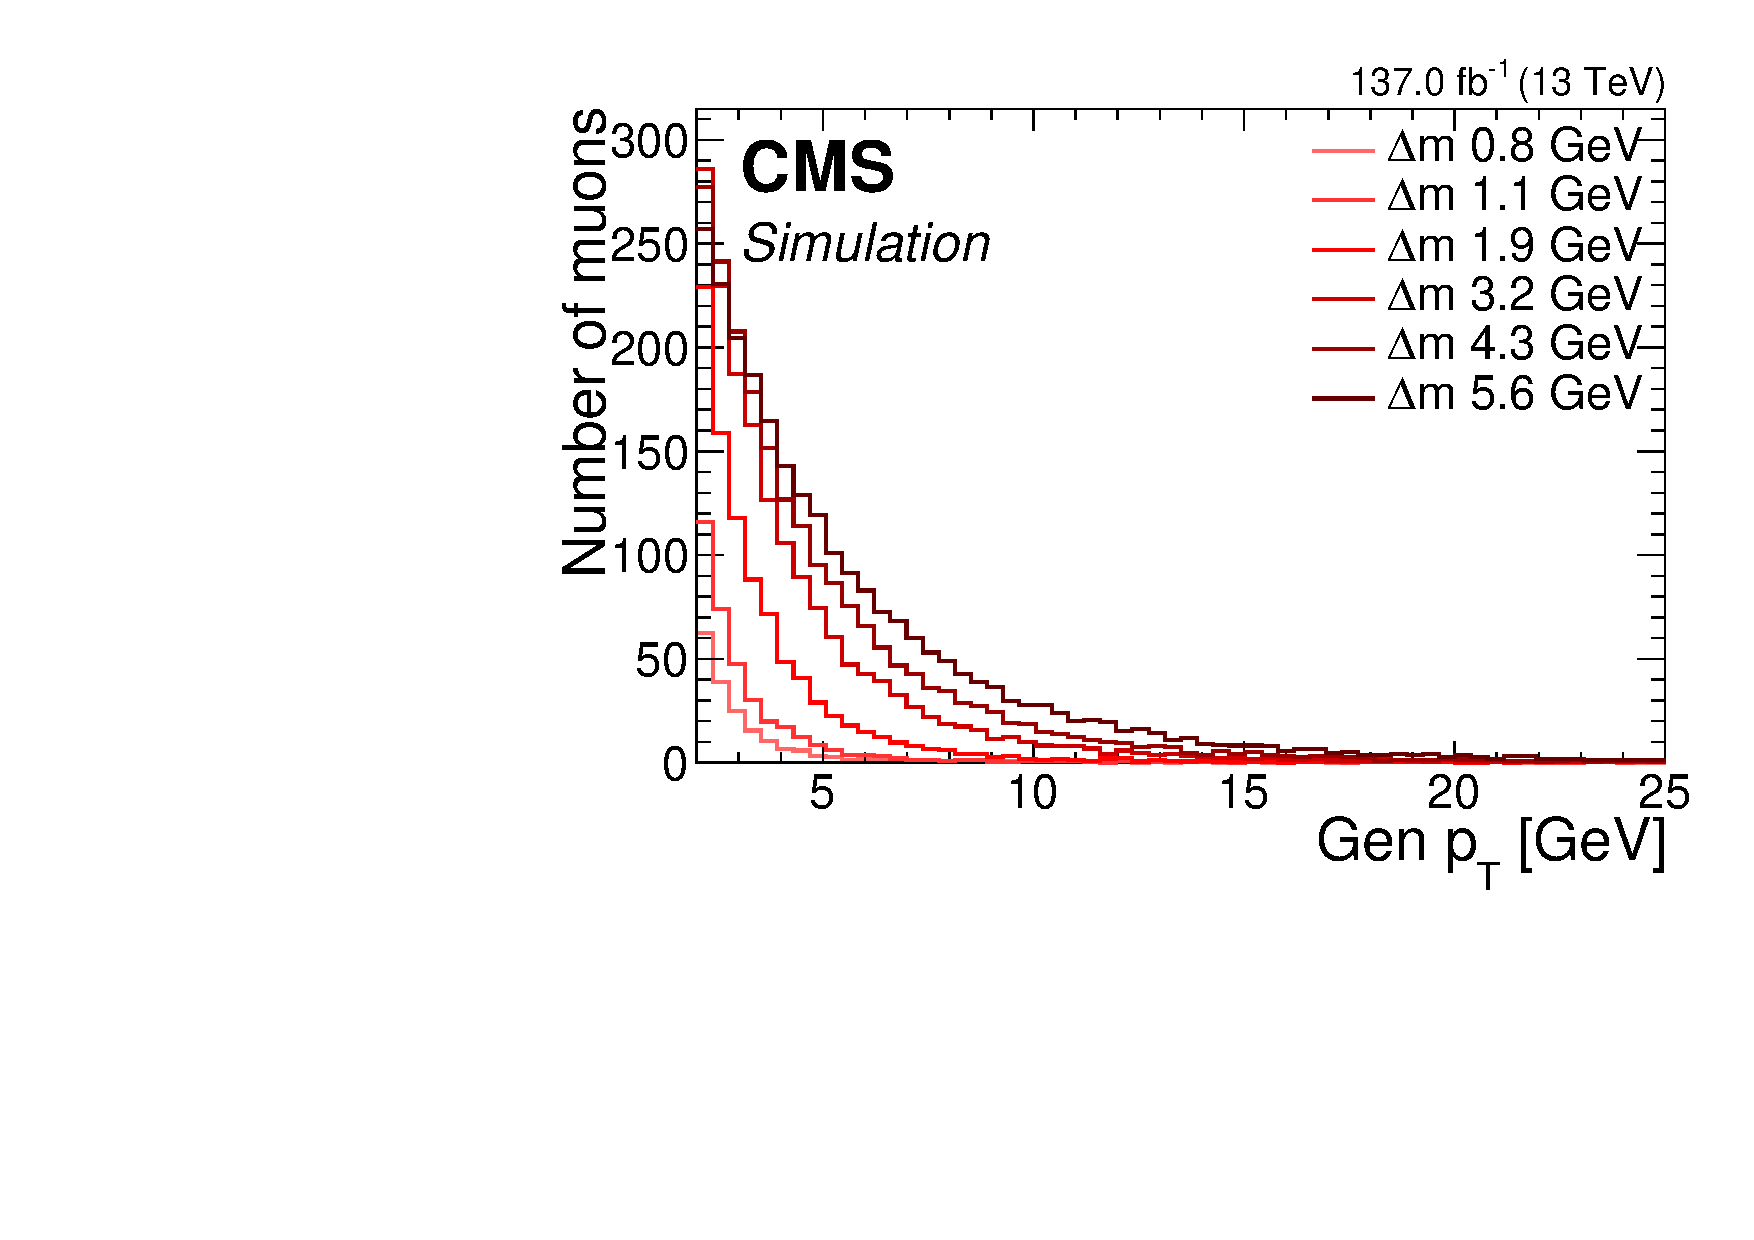
\includegraphics[width=0.32\linewidth]{plots/signal_muons_gen/none_Muons_pt.pdf} \,
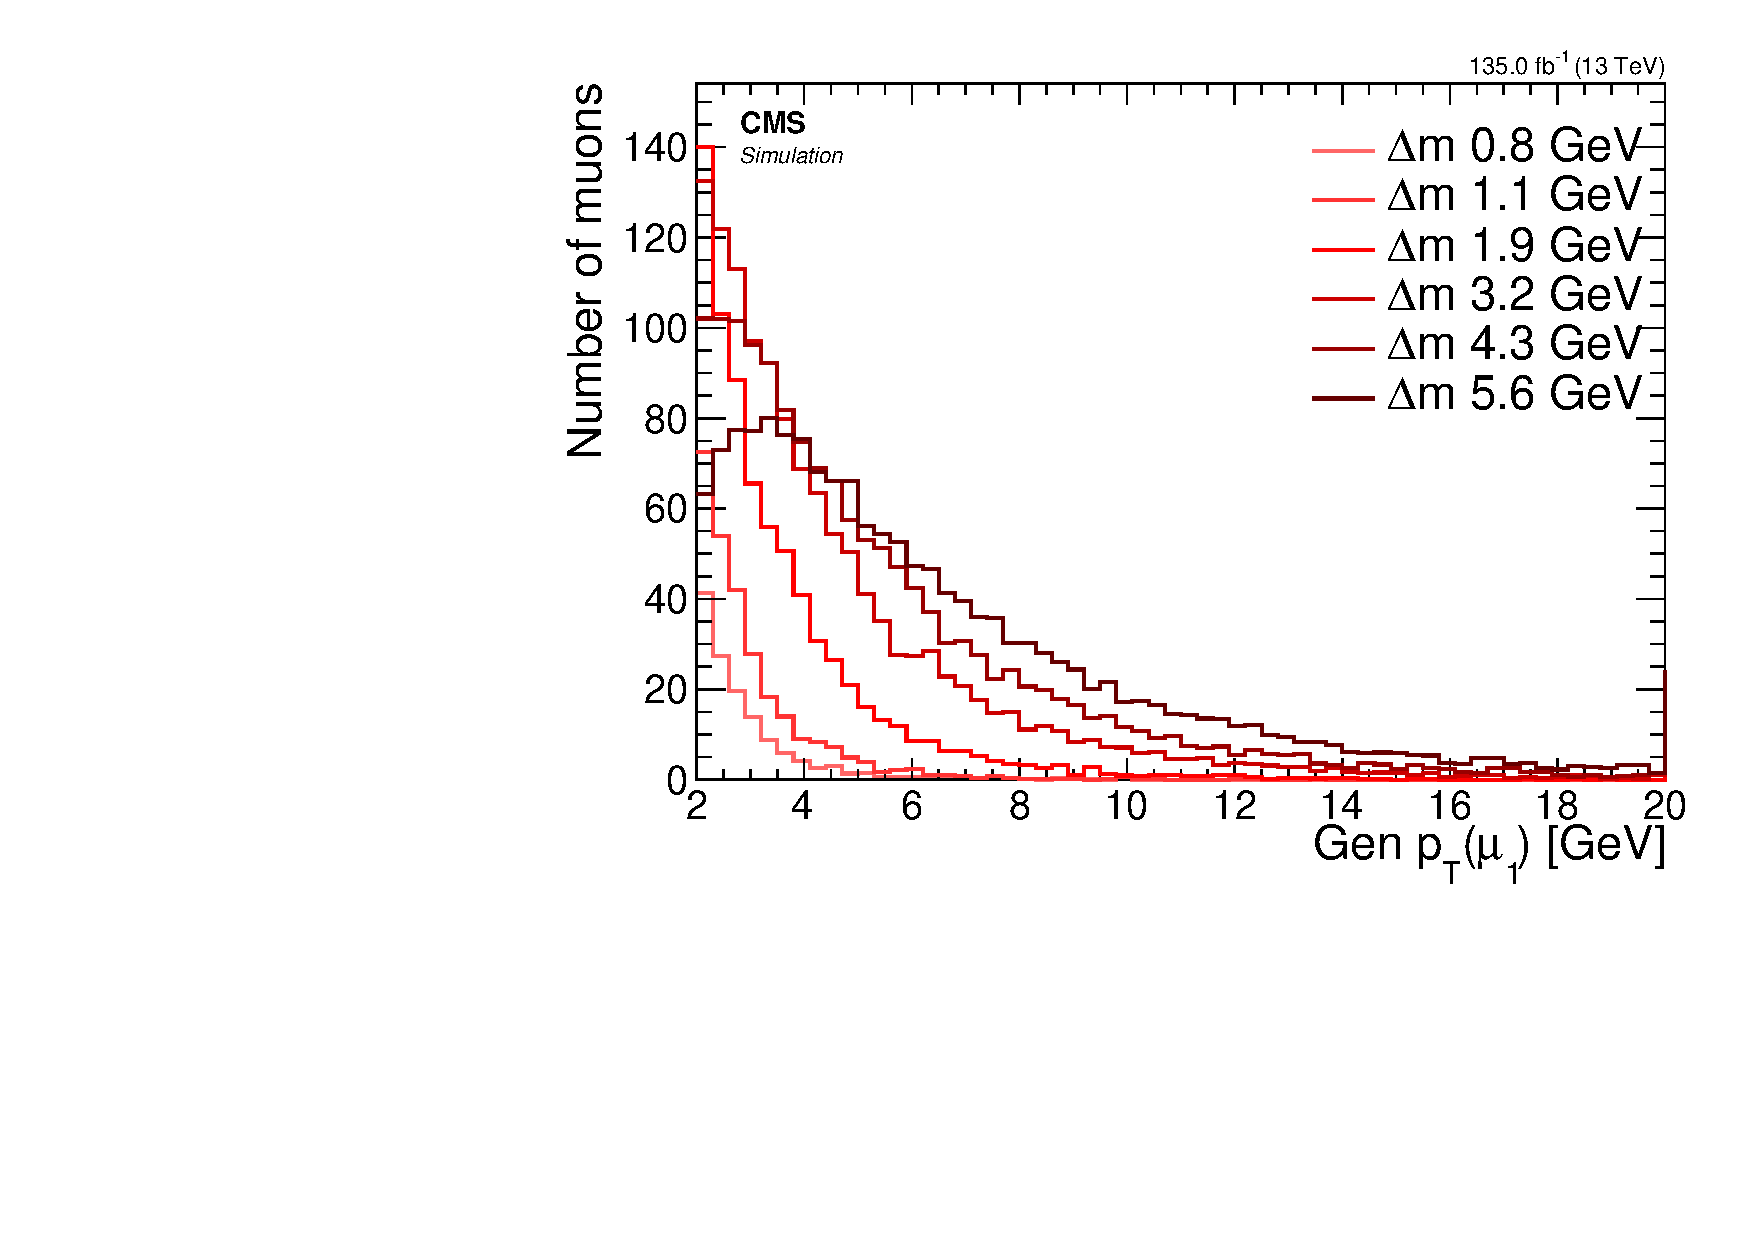
\includegraphics[width=0.32\linewidth]{plots/signal_muons_gen/none_Muons_m1_pt.pdf}  \,
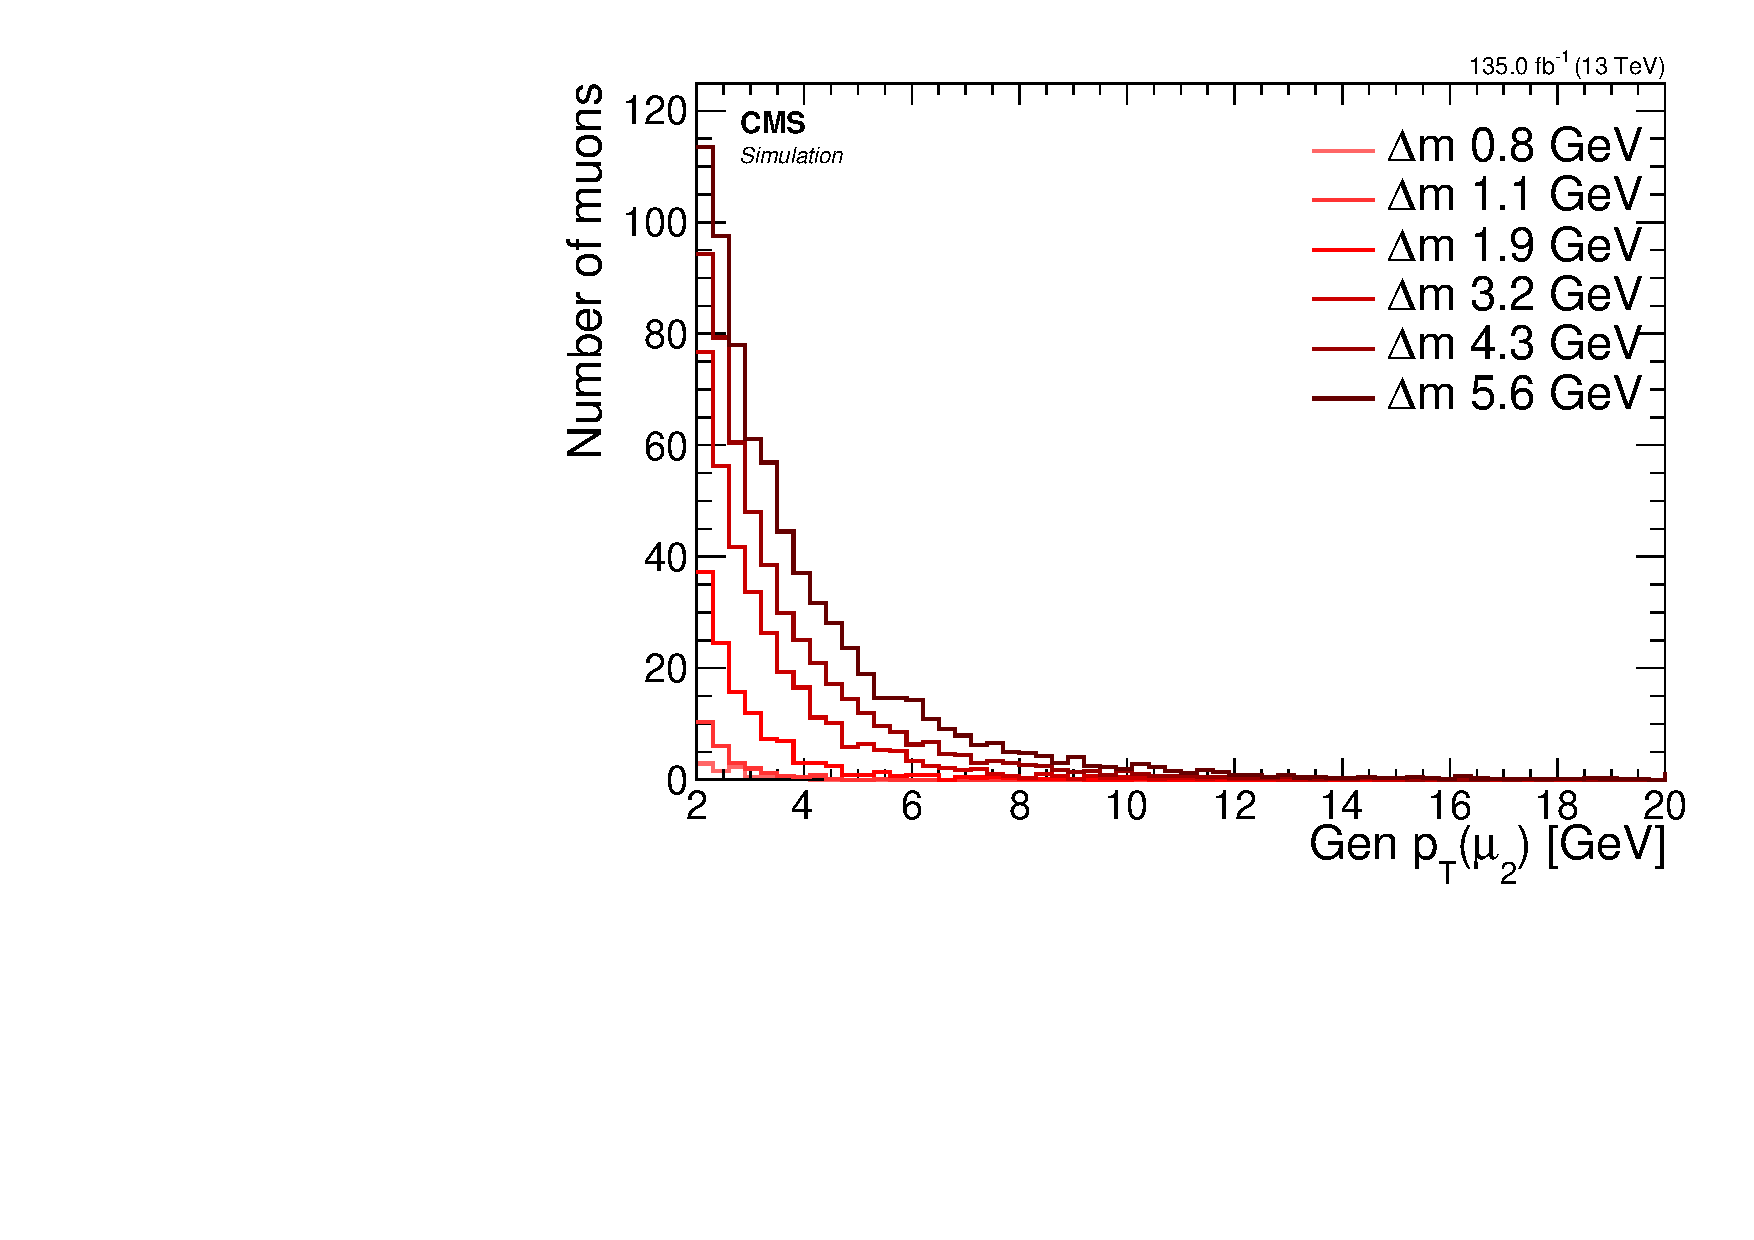
\includegraphics[width=0.32\linewidth]{plots/signal_muons_gen/none_Muons_m2_pt.pdf} \\
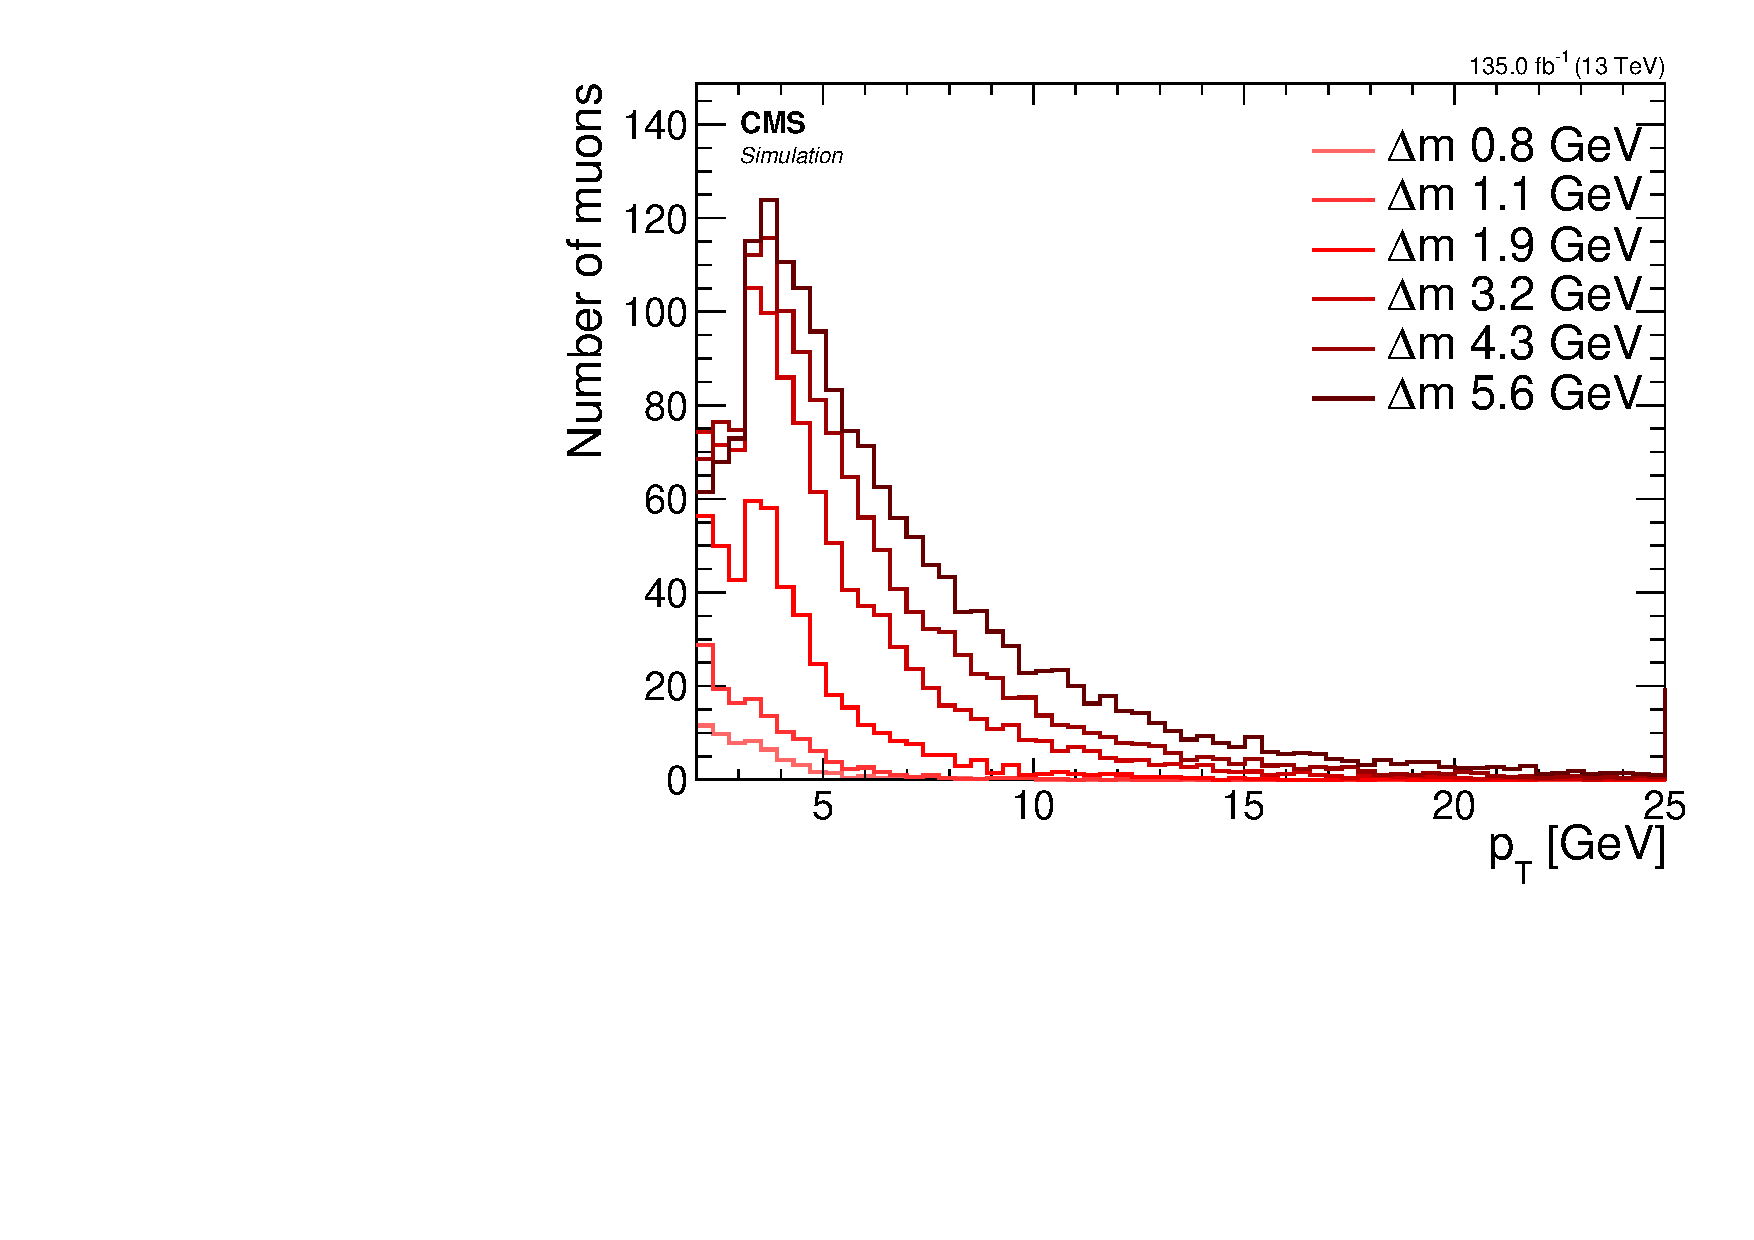
\includegraphics[width=0.32\linewidth]{plots/signal_muons/none_Muons_pt.pdf} \,
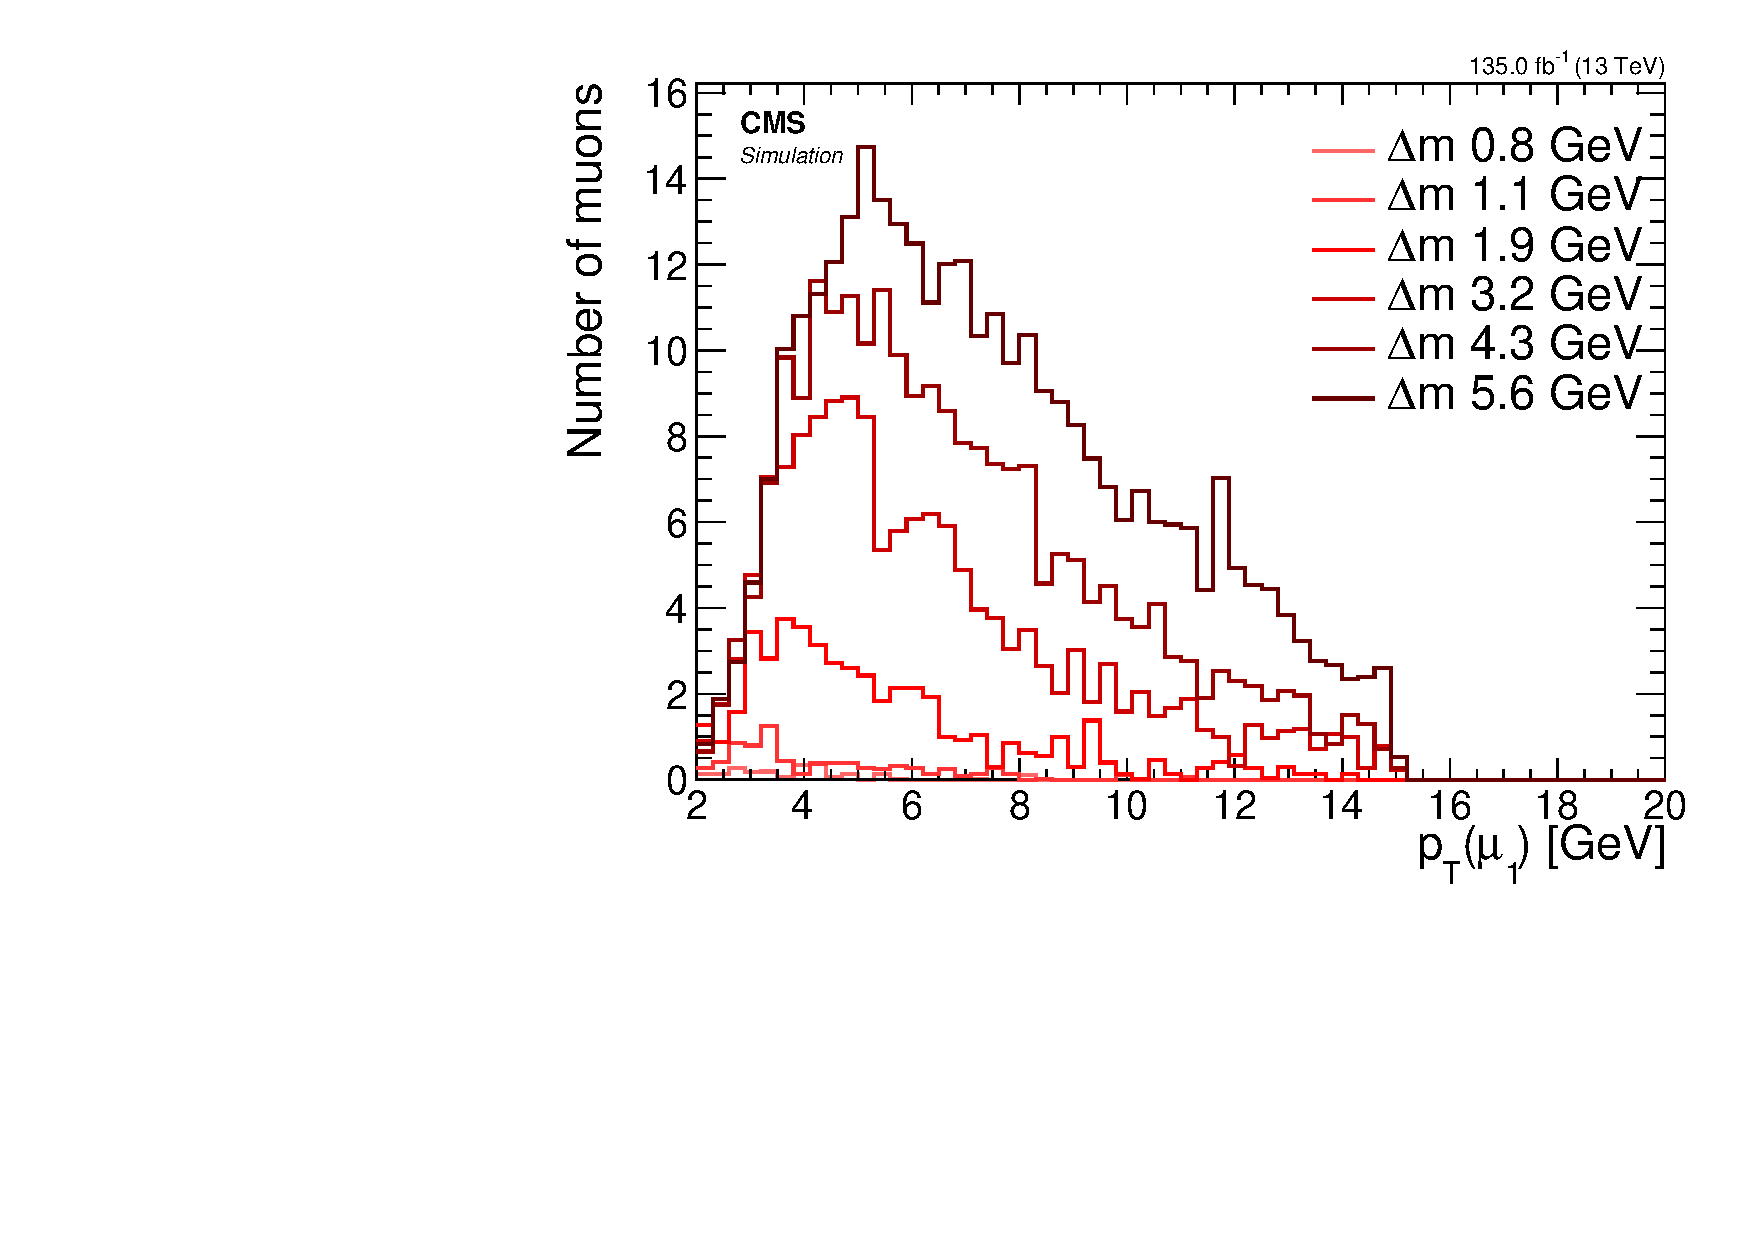
\includegraphics[width=0.32\linewidth]{plots/signal_muons/none_Muons_m1_pt.pdf}  \,
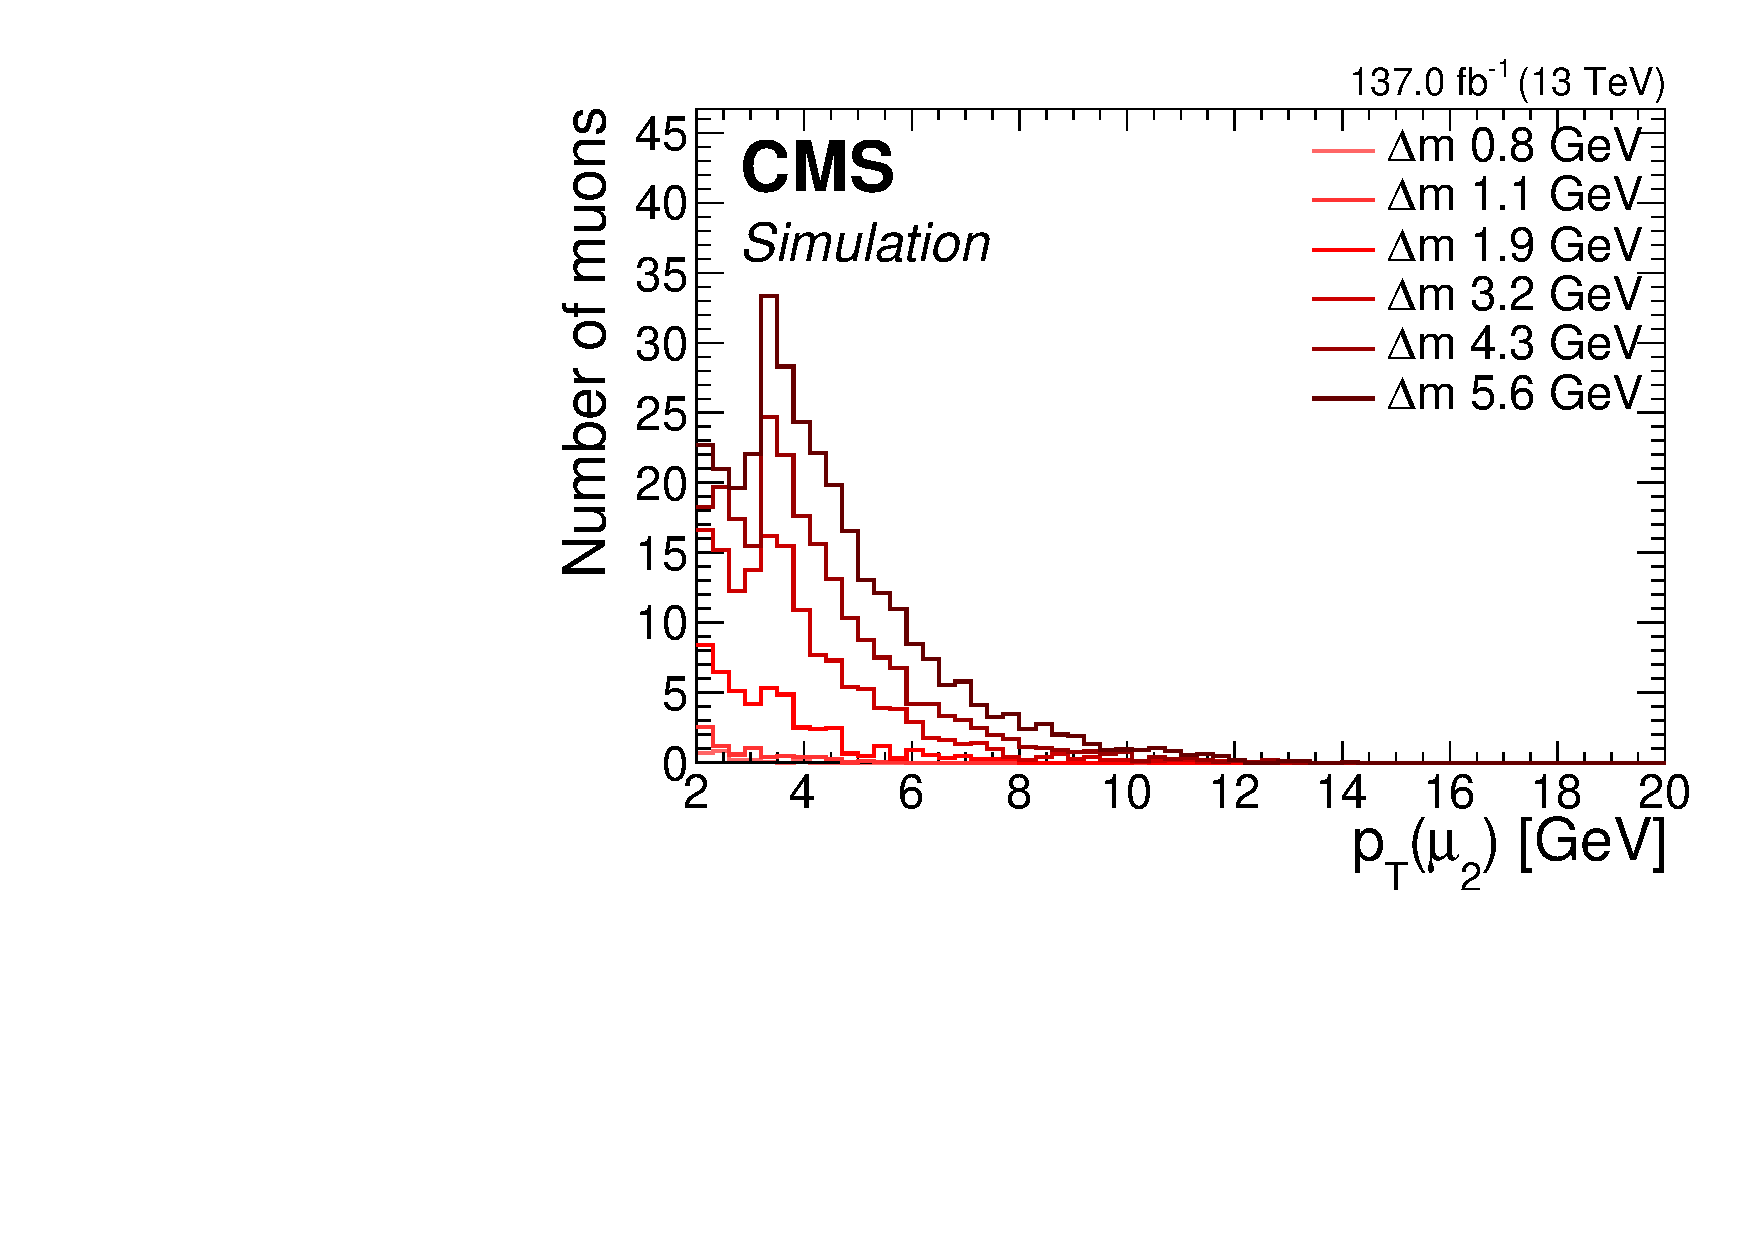
\includegraphics[width=0.32\linewidth]{plots/signal_muons/none_Muons_m2_pt.pdf} \\
\caption[Signal \pt distributions]{ Signal \pt distributions for inclusive (left), leading muon $\mu_1$ (middle),  subleading muon $\mu_2$ (right) at generator level (top) and reconstruction level passing analysis selection (bottom). }
\label{fig:signal-muons-pt}
\end{figure}

By comparing the generator level to the reconstruction level of the inclusive \pt distribution, we see that a reshaping occurs at around $3 \GeV$. A significant portion of the generated muons with $\pt<3\GeV$ are being lost in reconstruction. The reconstructed subleading \pt distribution has a camel shape whereby the efficiency drops bellow \pt of $3\GeV$ and only partially regained at $\pt<3\GeV$. This is a detector effect and can be seen more clearly when we split the \pt distribution into a barrel ($\abs{\eta} < 1.2$) and encaps ($\abs{\eta} \geq 1.2$) portions.

\begin{figure}[!htb]
\centering
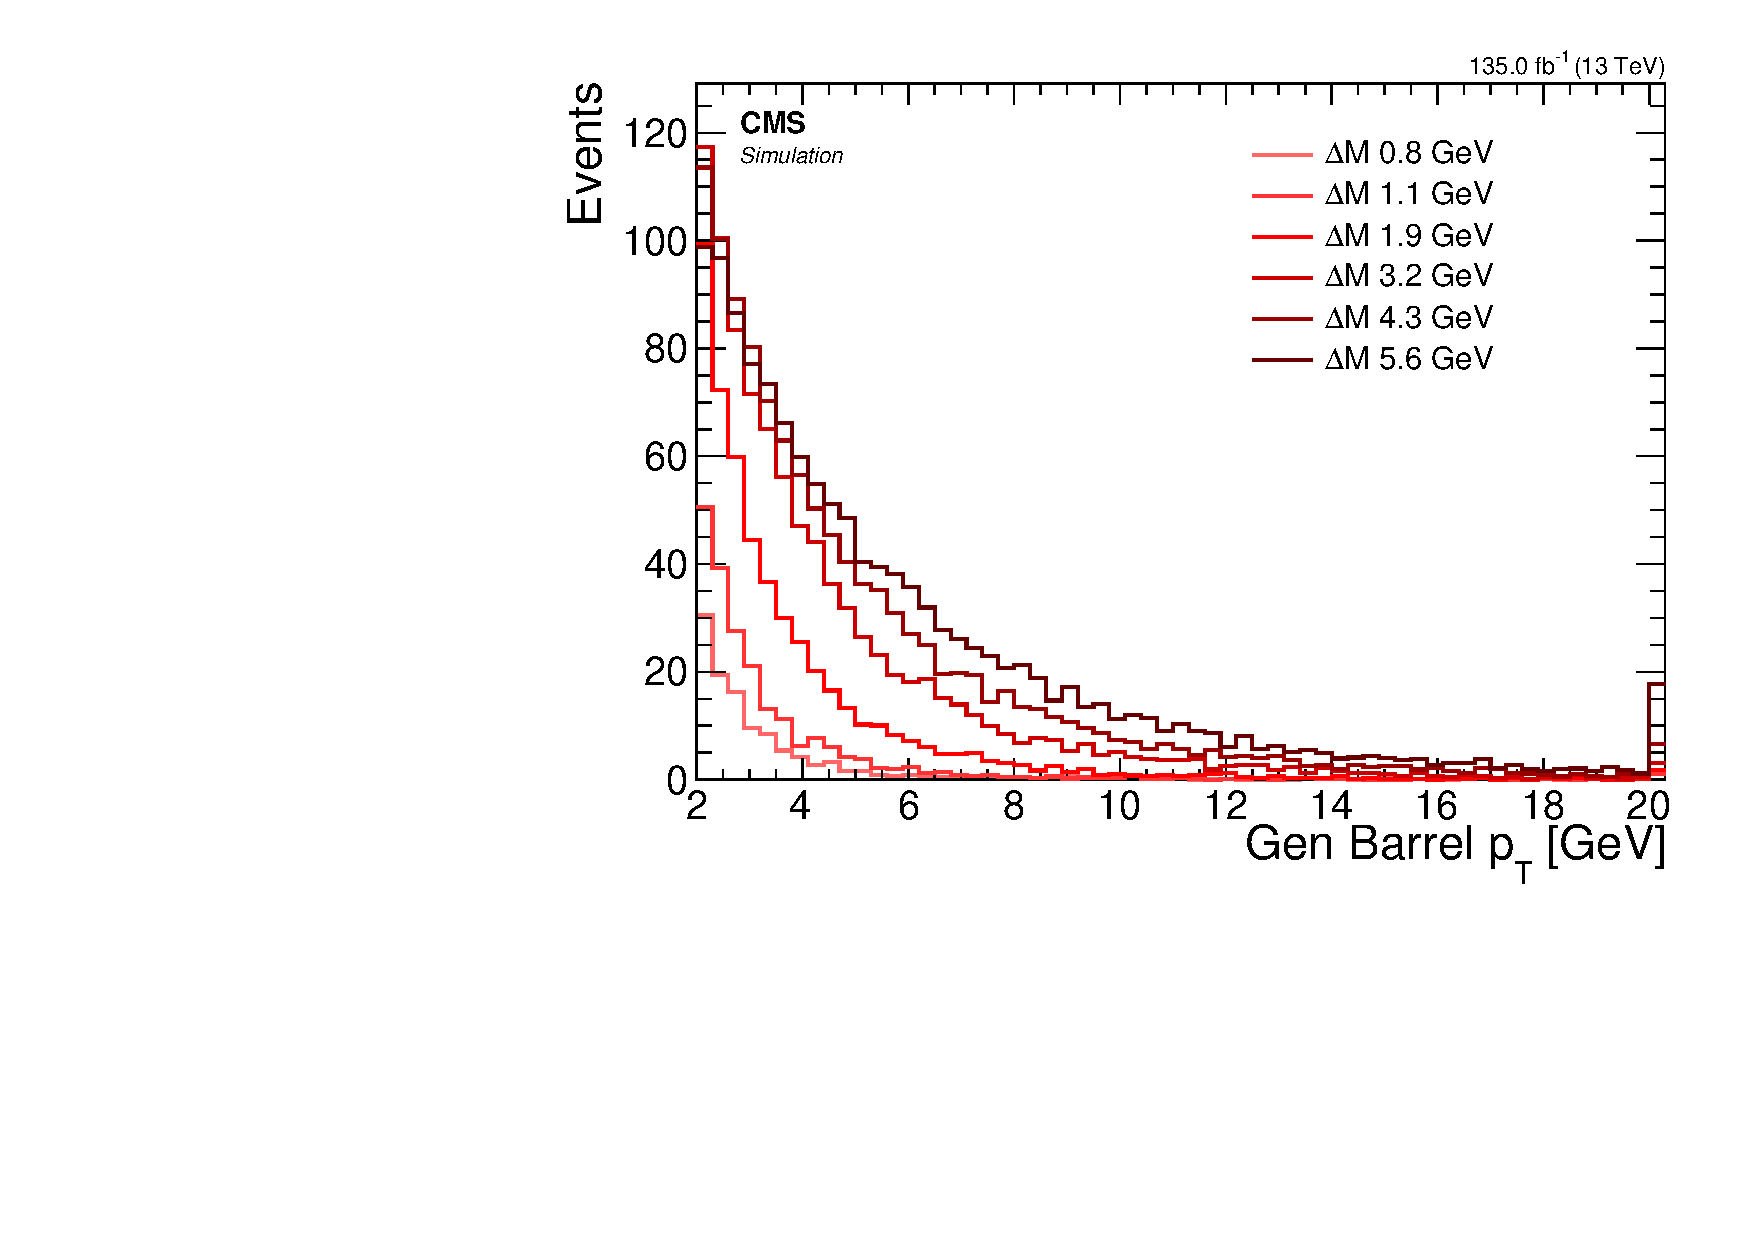
\includegraphics[width=0.48\linewidth]{plots/signal_muons_gen/none_Muons_pt_barrel.pdf} \,
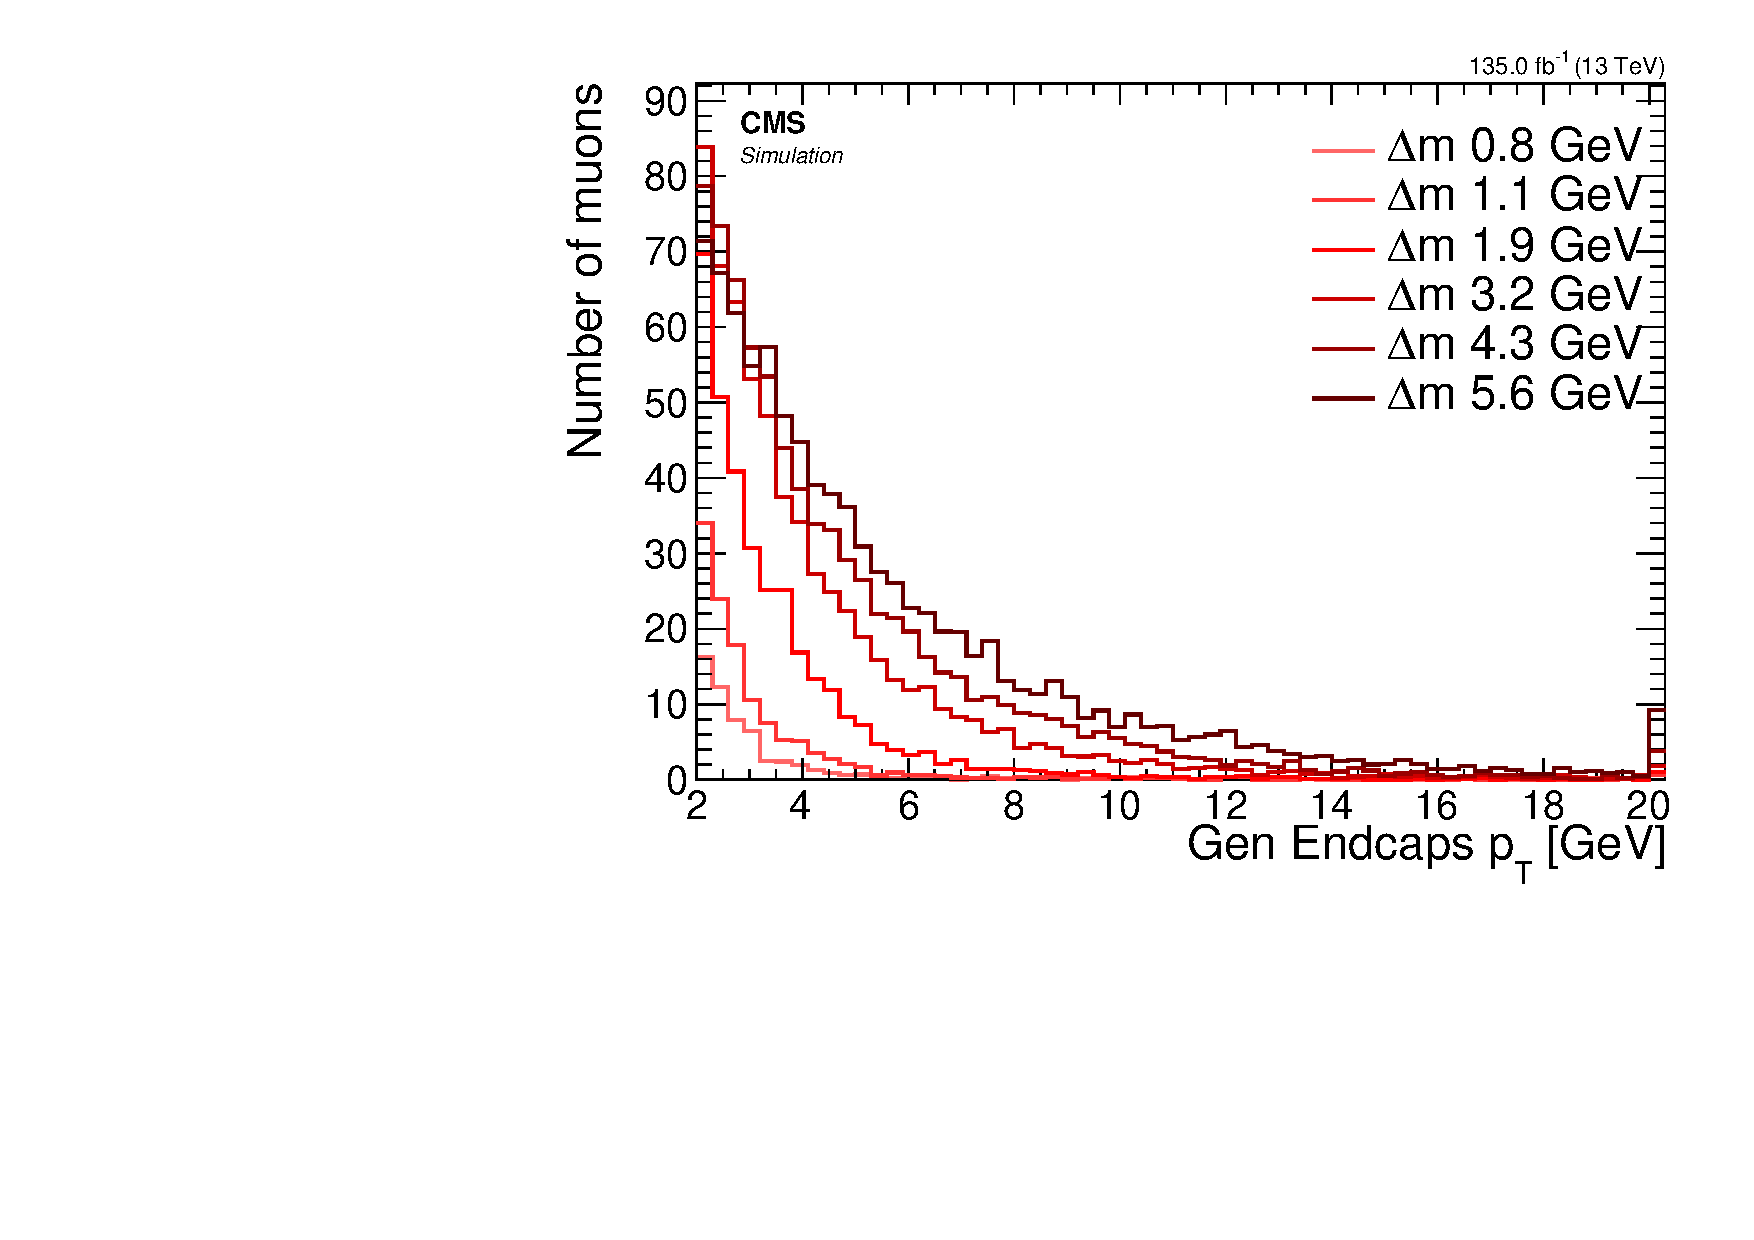
\includegraphics[width=0.48\linewidth]{plots/signal_muons_gen/none_Muons_pt_endcape.pdf}  \\
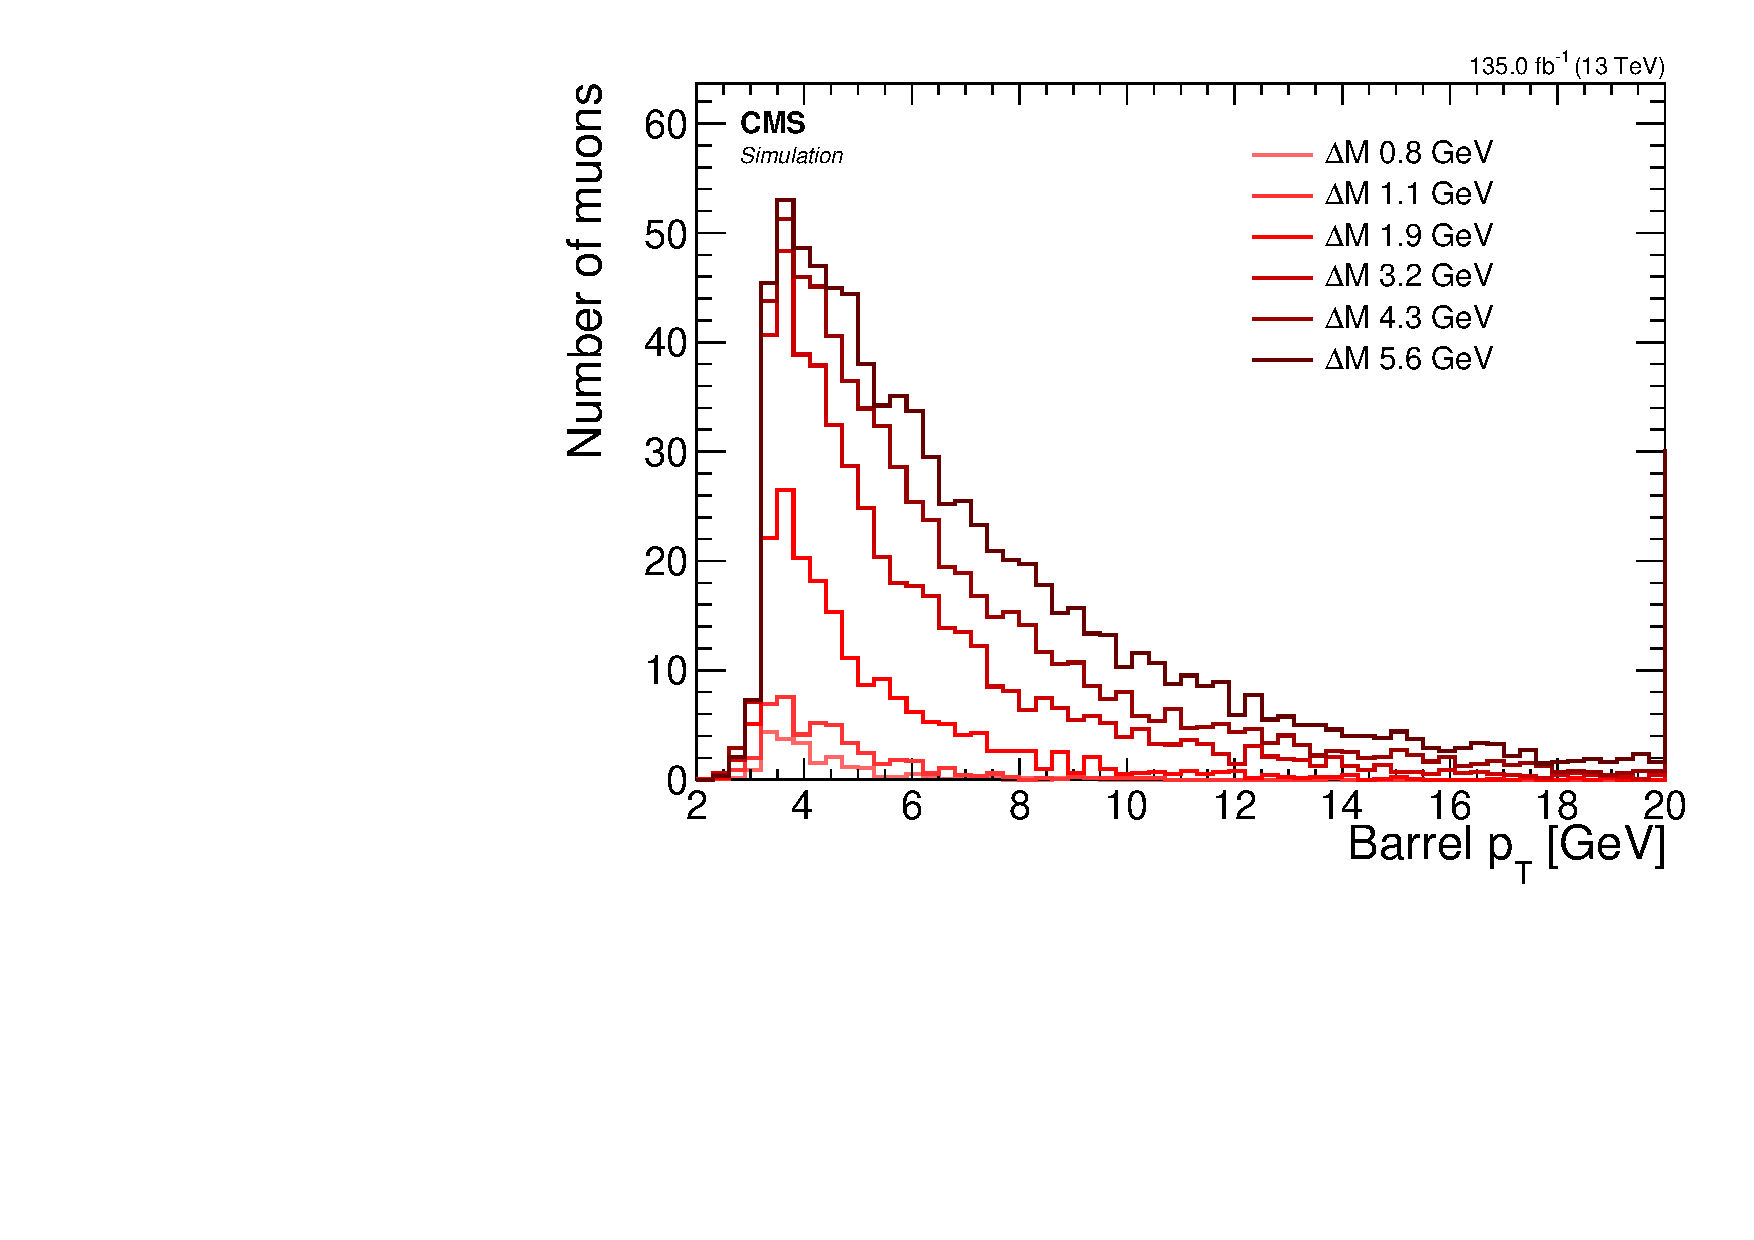
\includegraphics[width=0.48\linewidth]{plots/signal_muons/none_Muons_pt_barrel.pdf} \,
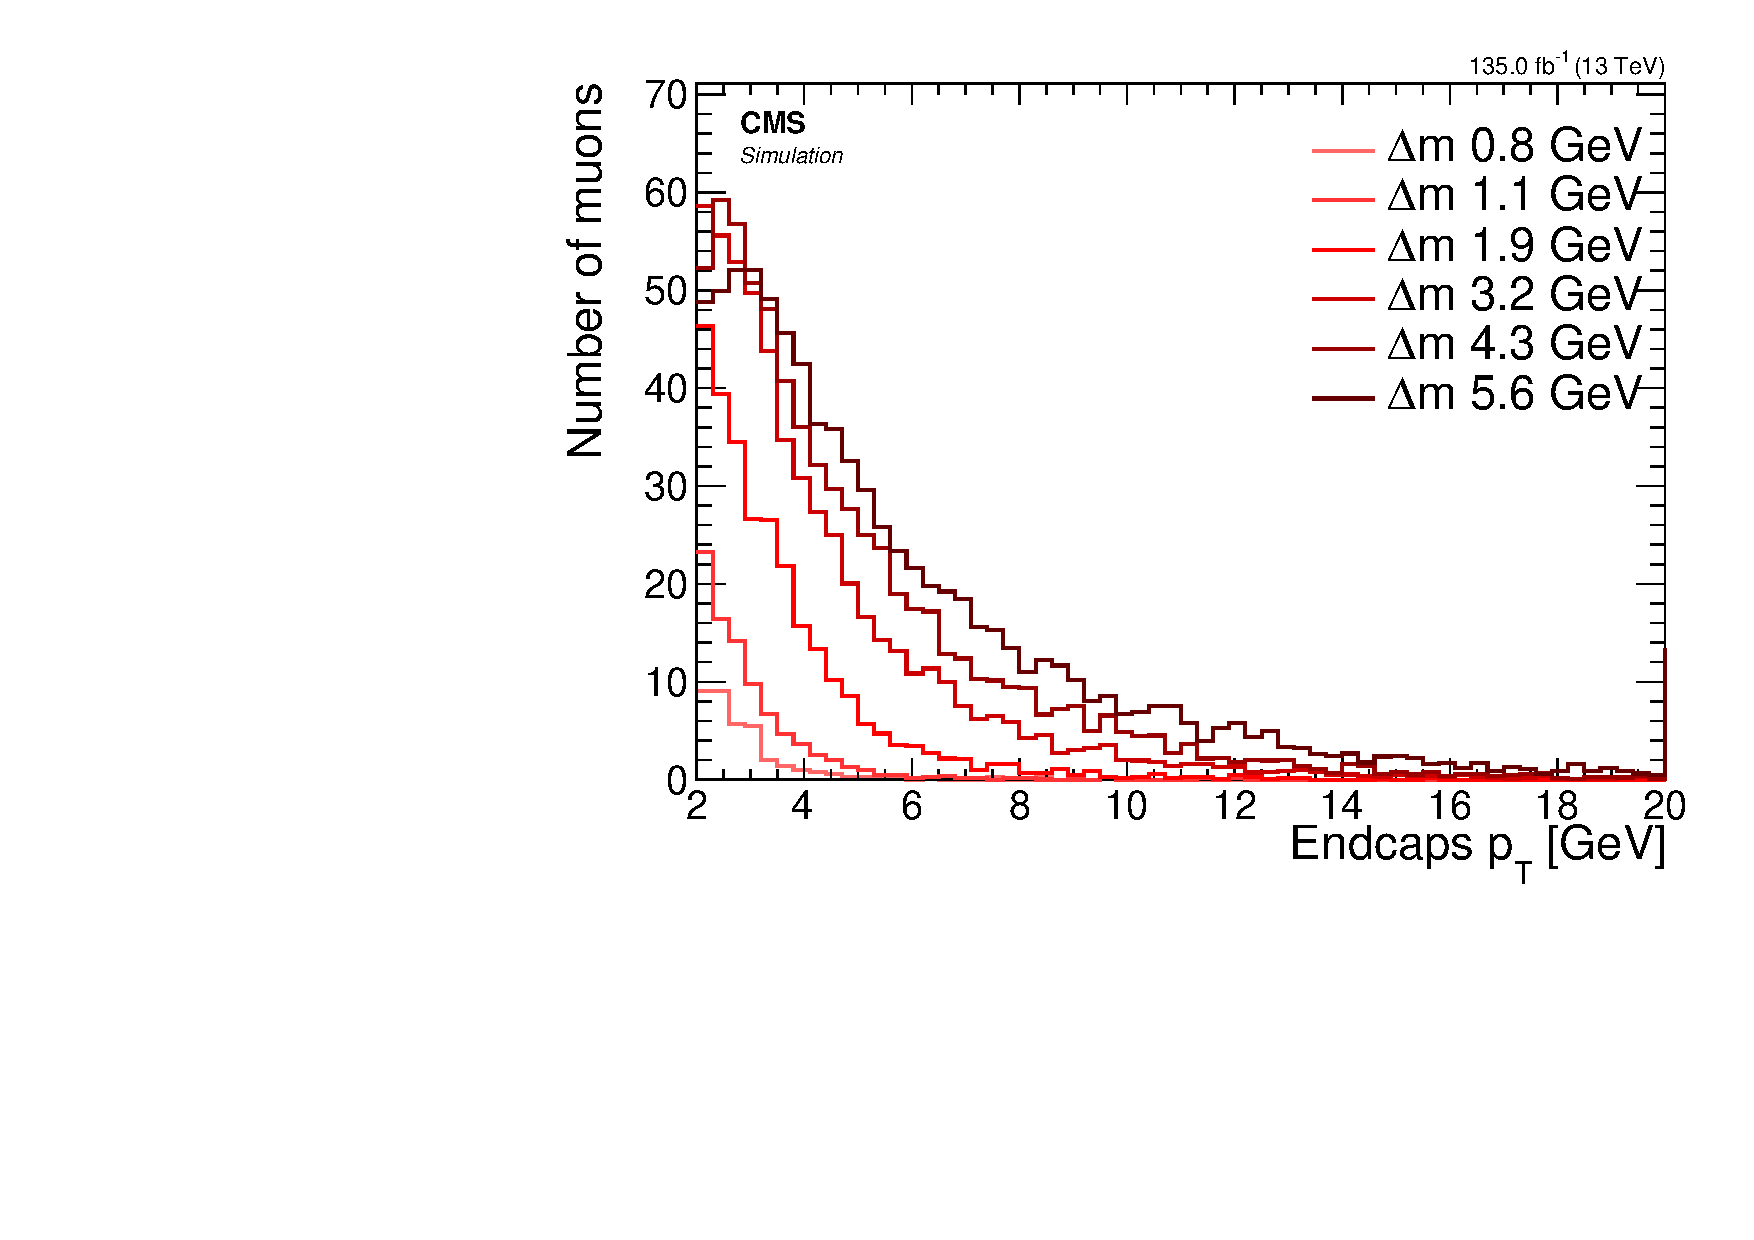
\includegraphics[width=0.48\linewidth]{plots/signal_muons/none_Muons_pt_endcape.pdf}  \\
\caption[Signal \pt distributions split into barrel and endcaps]{ Signal inclusive \pt distributions for barrel $\abs{\eta} < 1.2$ (left) and endcaps $\abs{\eta} \geq 1.2$ (right) at generator level (top) and reconstruction level passing analysis selection (bottom).}
\label{fig:signal-pt-barrel-endcaps}
\end{figure}

The picture becomes much clearer in regards to the reconstruction efficiency as a function of \pt. When comparing the generator level distribution of the barrel muons on the top left with its constructed counterpart on the bottom left, we see that the barrel is almost completely unable to reconstruct muons with $\pt < 3\GeV$, while the endcaps, shown on the left, are able to do so. As we will see in the \gls{mll} and \gls{dr} upcoming sections (\ref{sec:gen-invariant-mass} and \ref{sec:lepton-dr}), since those distribution have an important relationship, that has consequences in regards to reshaping kinematic distributions, as well as signal acceptance in general. Since the low region of $2 \leq \pt \leq 3.5\GeV$ is crucial in giving us access to low \dm signal points, it is achieved, as can be seen here, mainly with the help of the muon chamber endcaps.

Since the barrel and endcaps are seperated by different regions of $\eta$, $\abs{\eta} < 1.2$ for barrel and $\abs{\eta} \geq 1.2$ for endcaps, it worth taking a look at the $\eta$ distributions of the muons as well.

\begin{figure}[!htb]
\centering
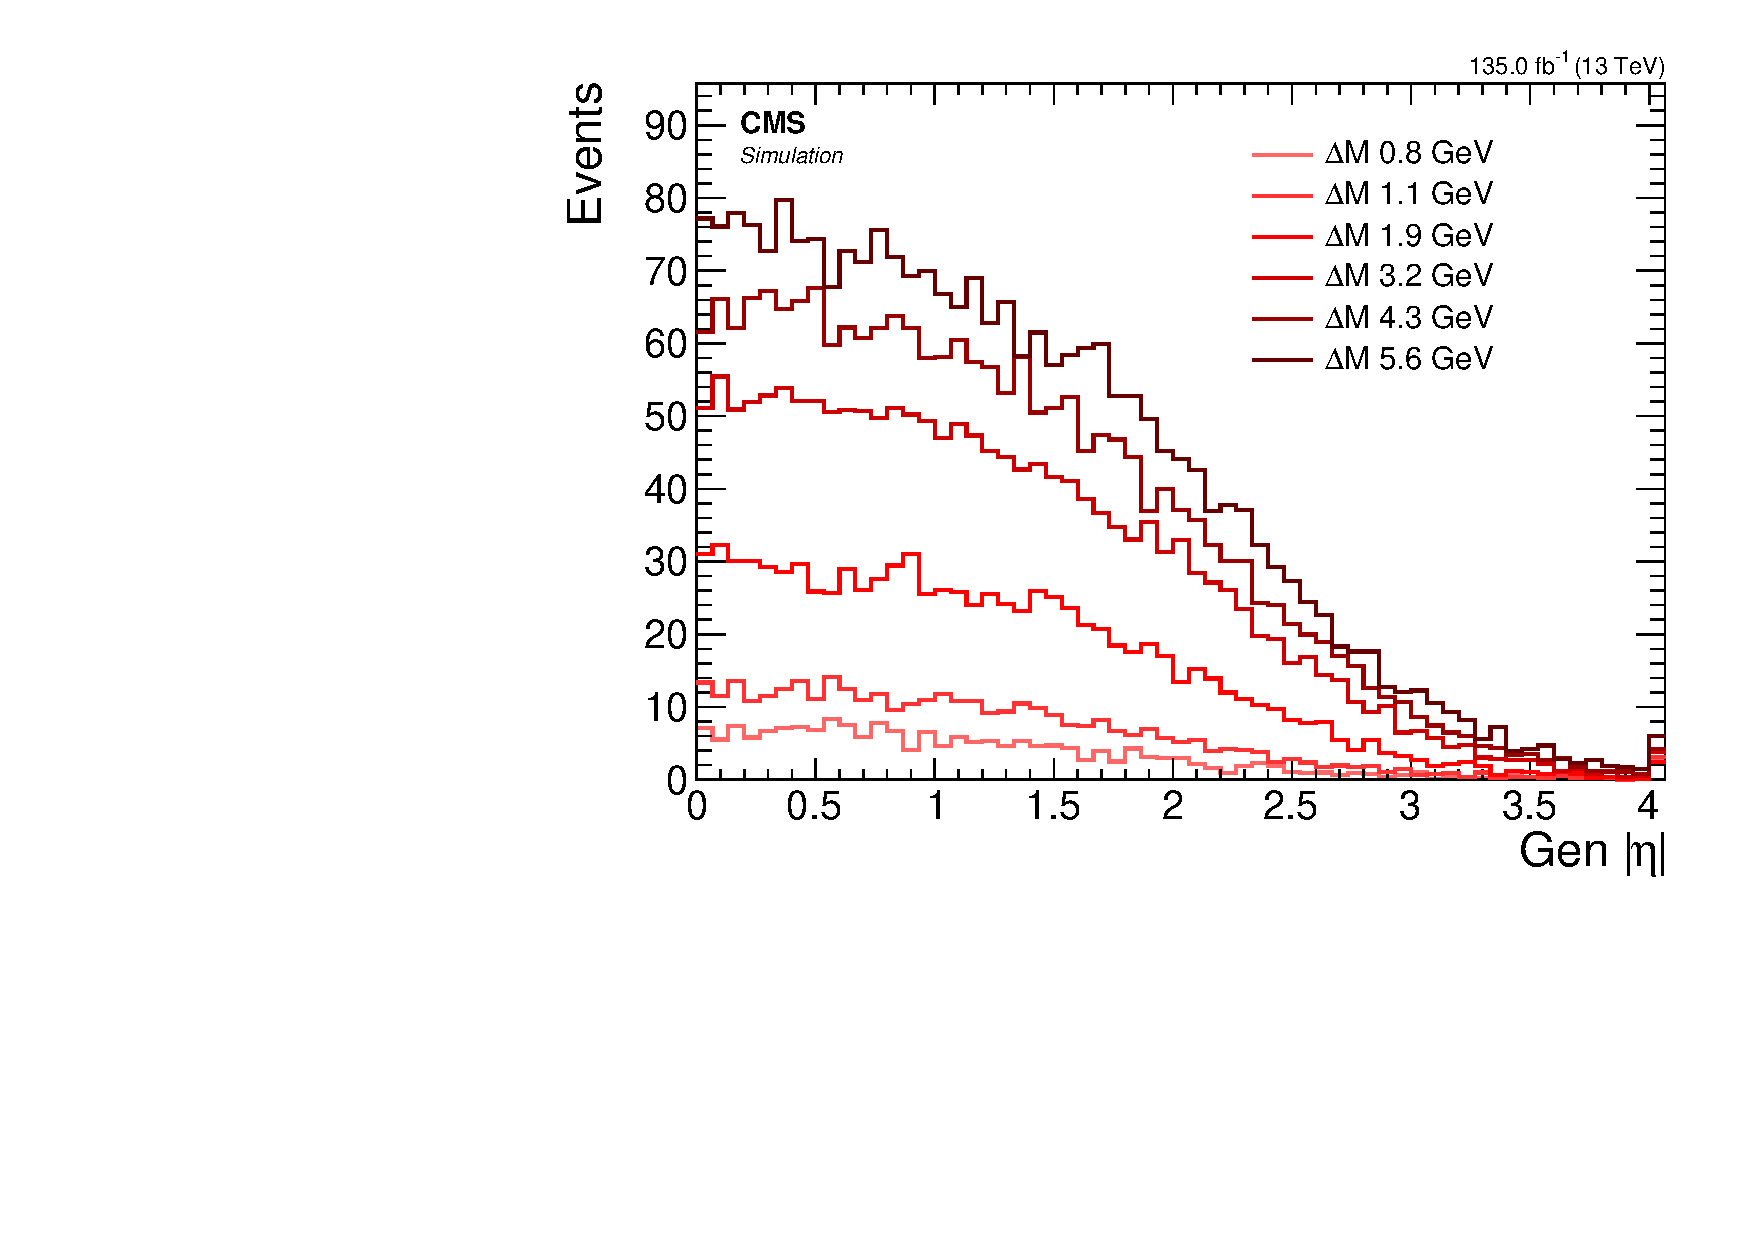
\includegraphics[width=0.32\linewidth]{plots/signal_muons_gen/none_Muons_Eta.pdf} \,
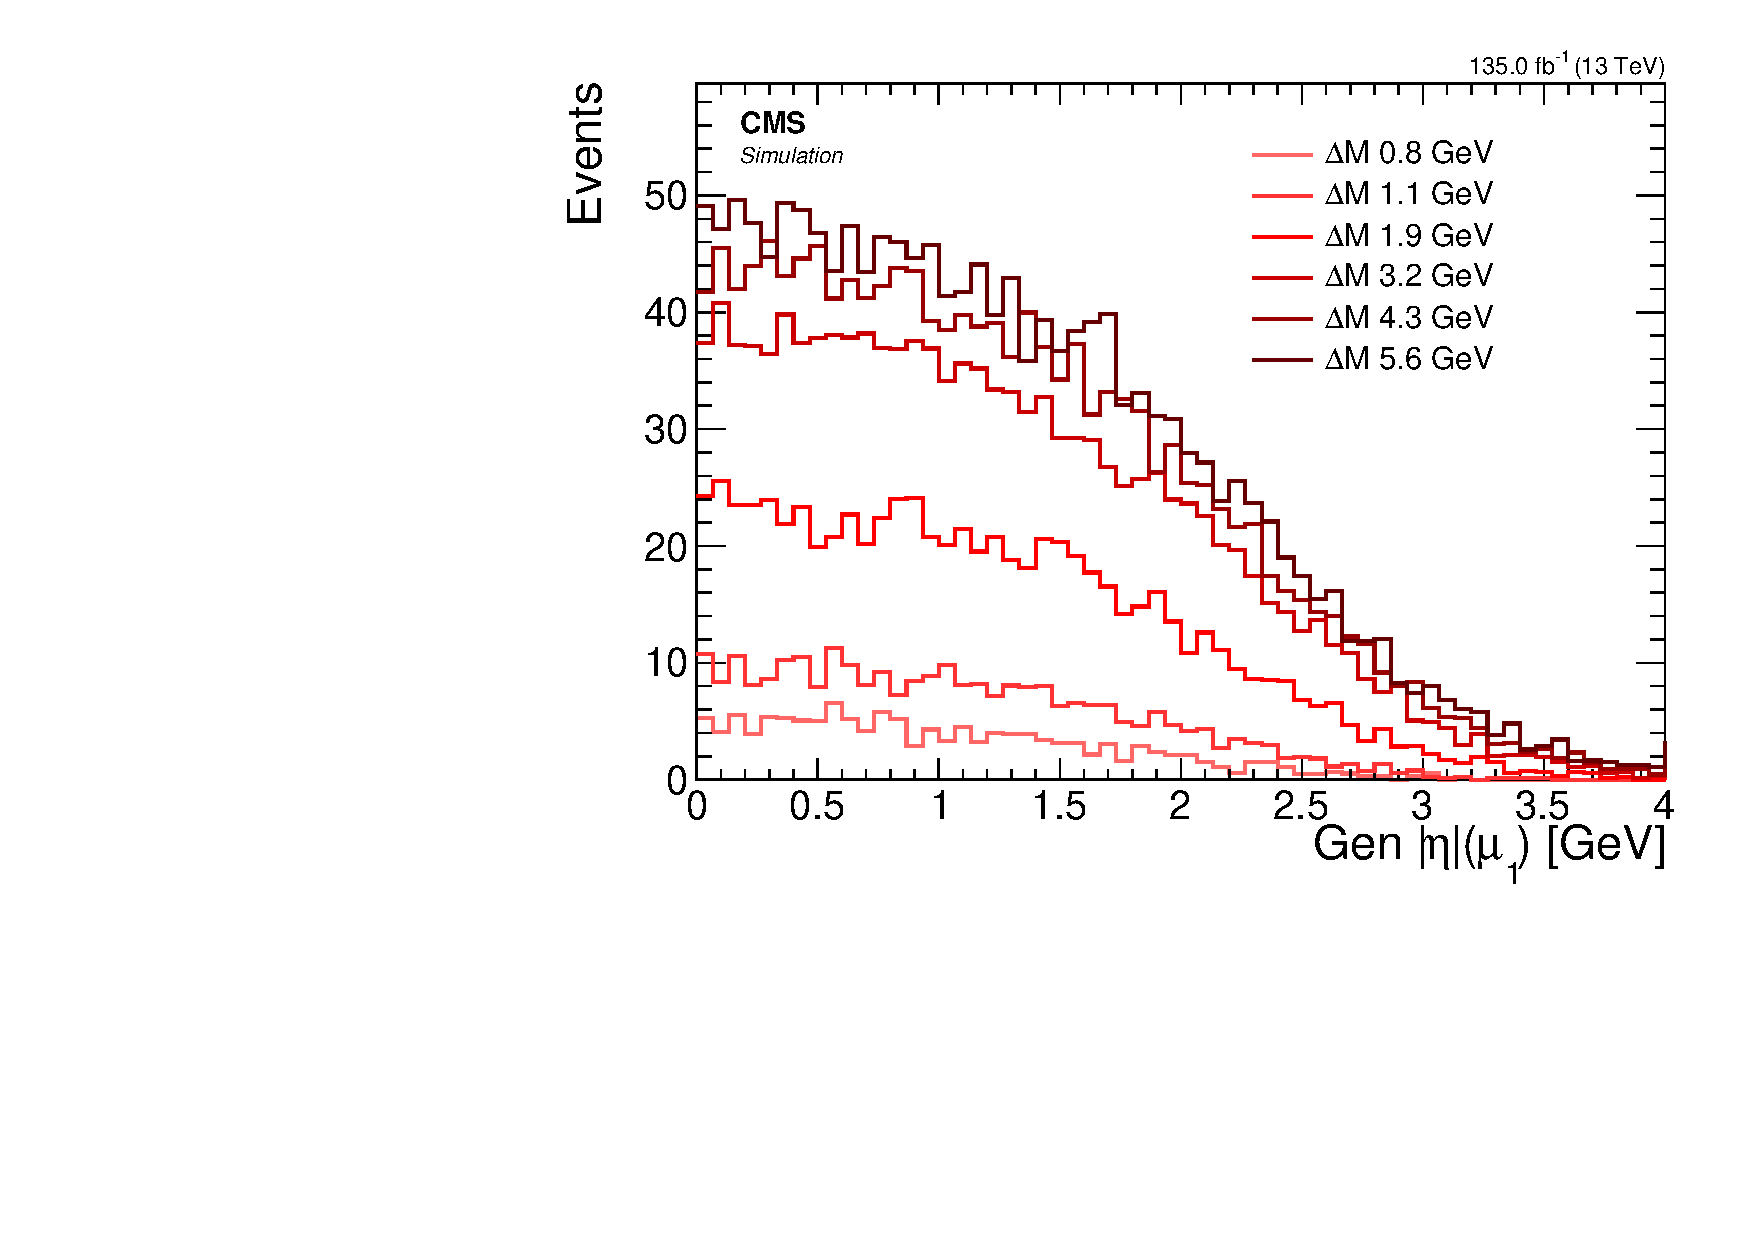
\includegraphics[width=0.32\linewidth]{plots/signal_muons_gen/none_Muons_m1_eta.pdf}  \,
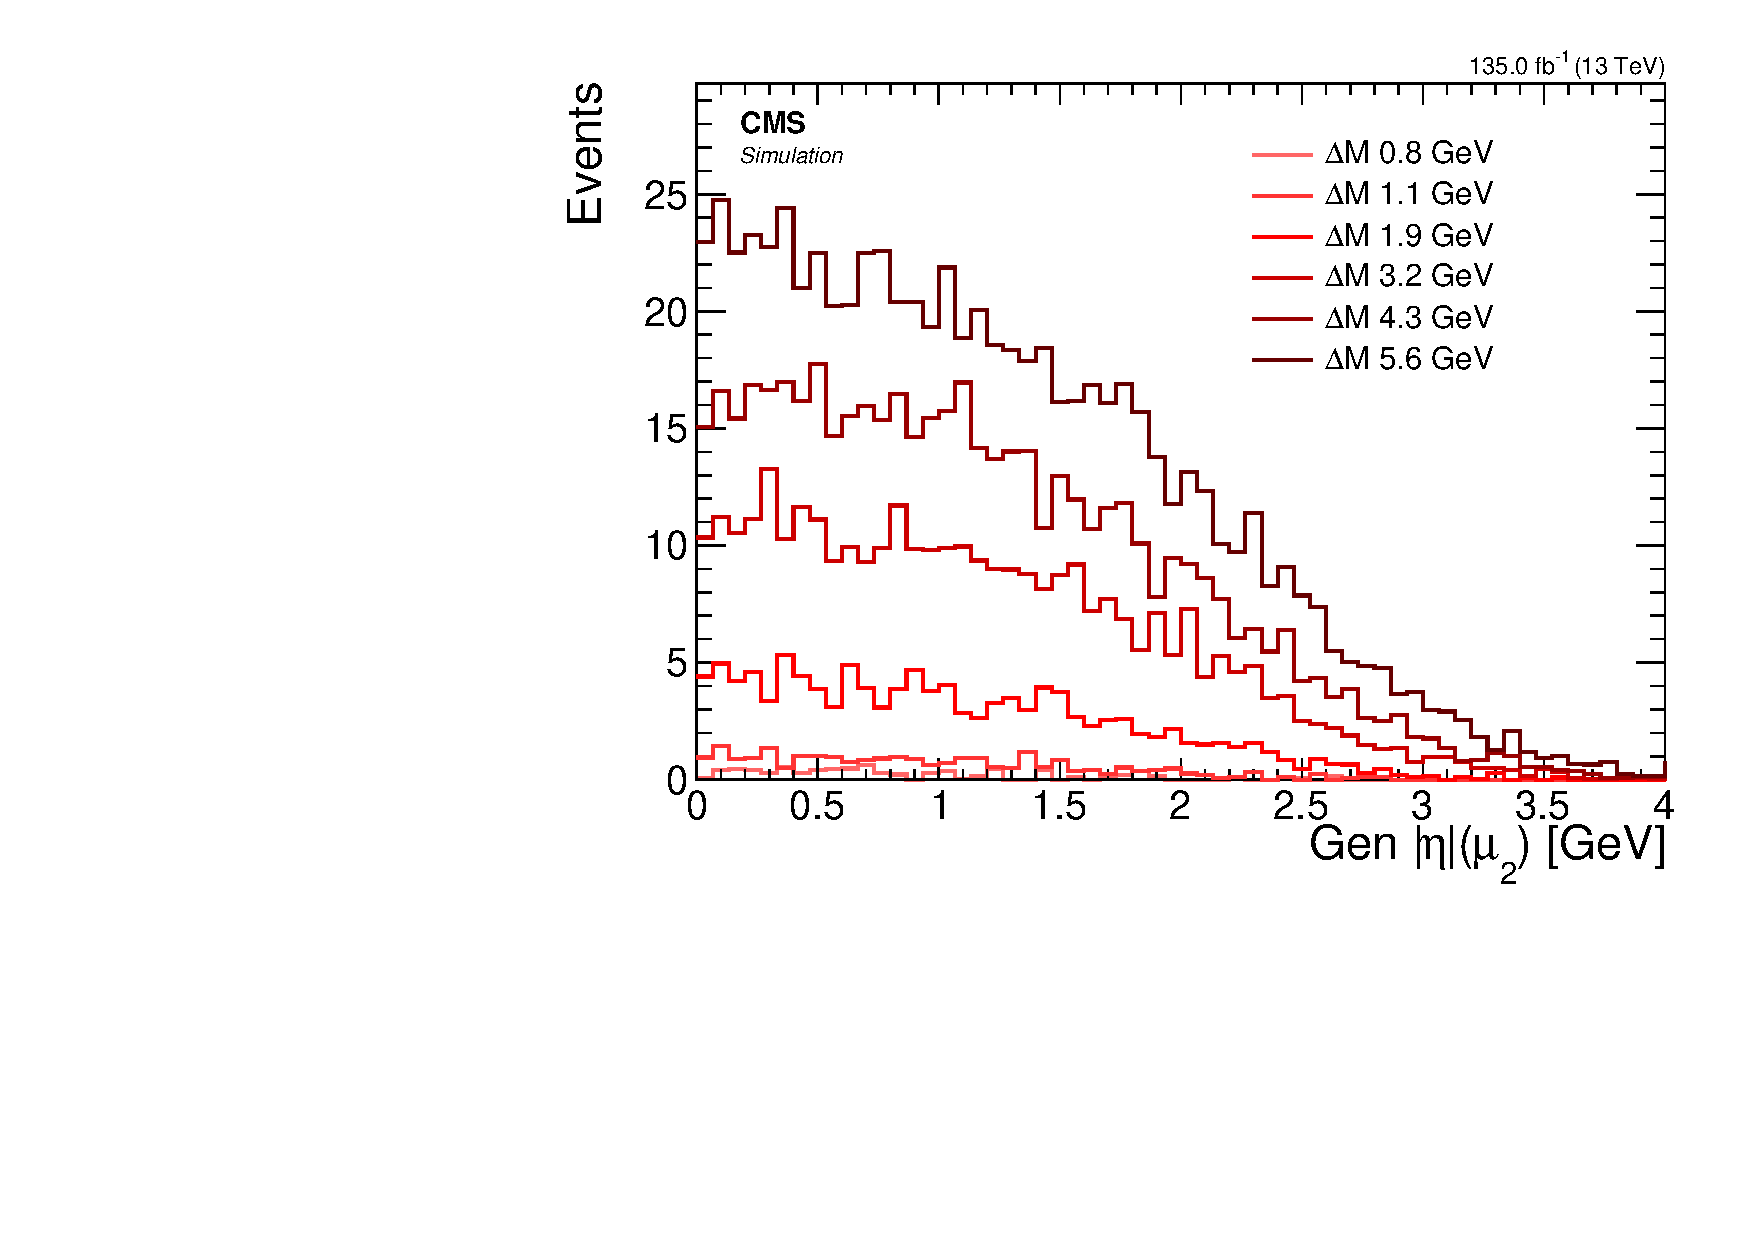
\includegraphics[width=0.32\linewidth]{plots/signal_muons_gen/none_Muons_m2_eta.pdf} \\
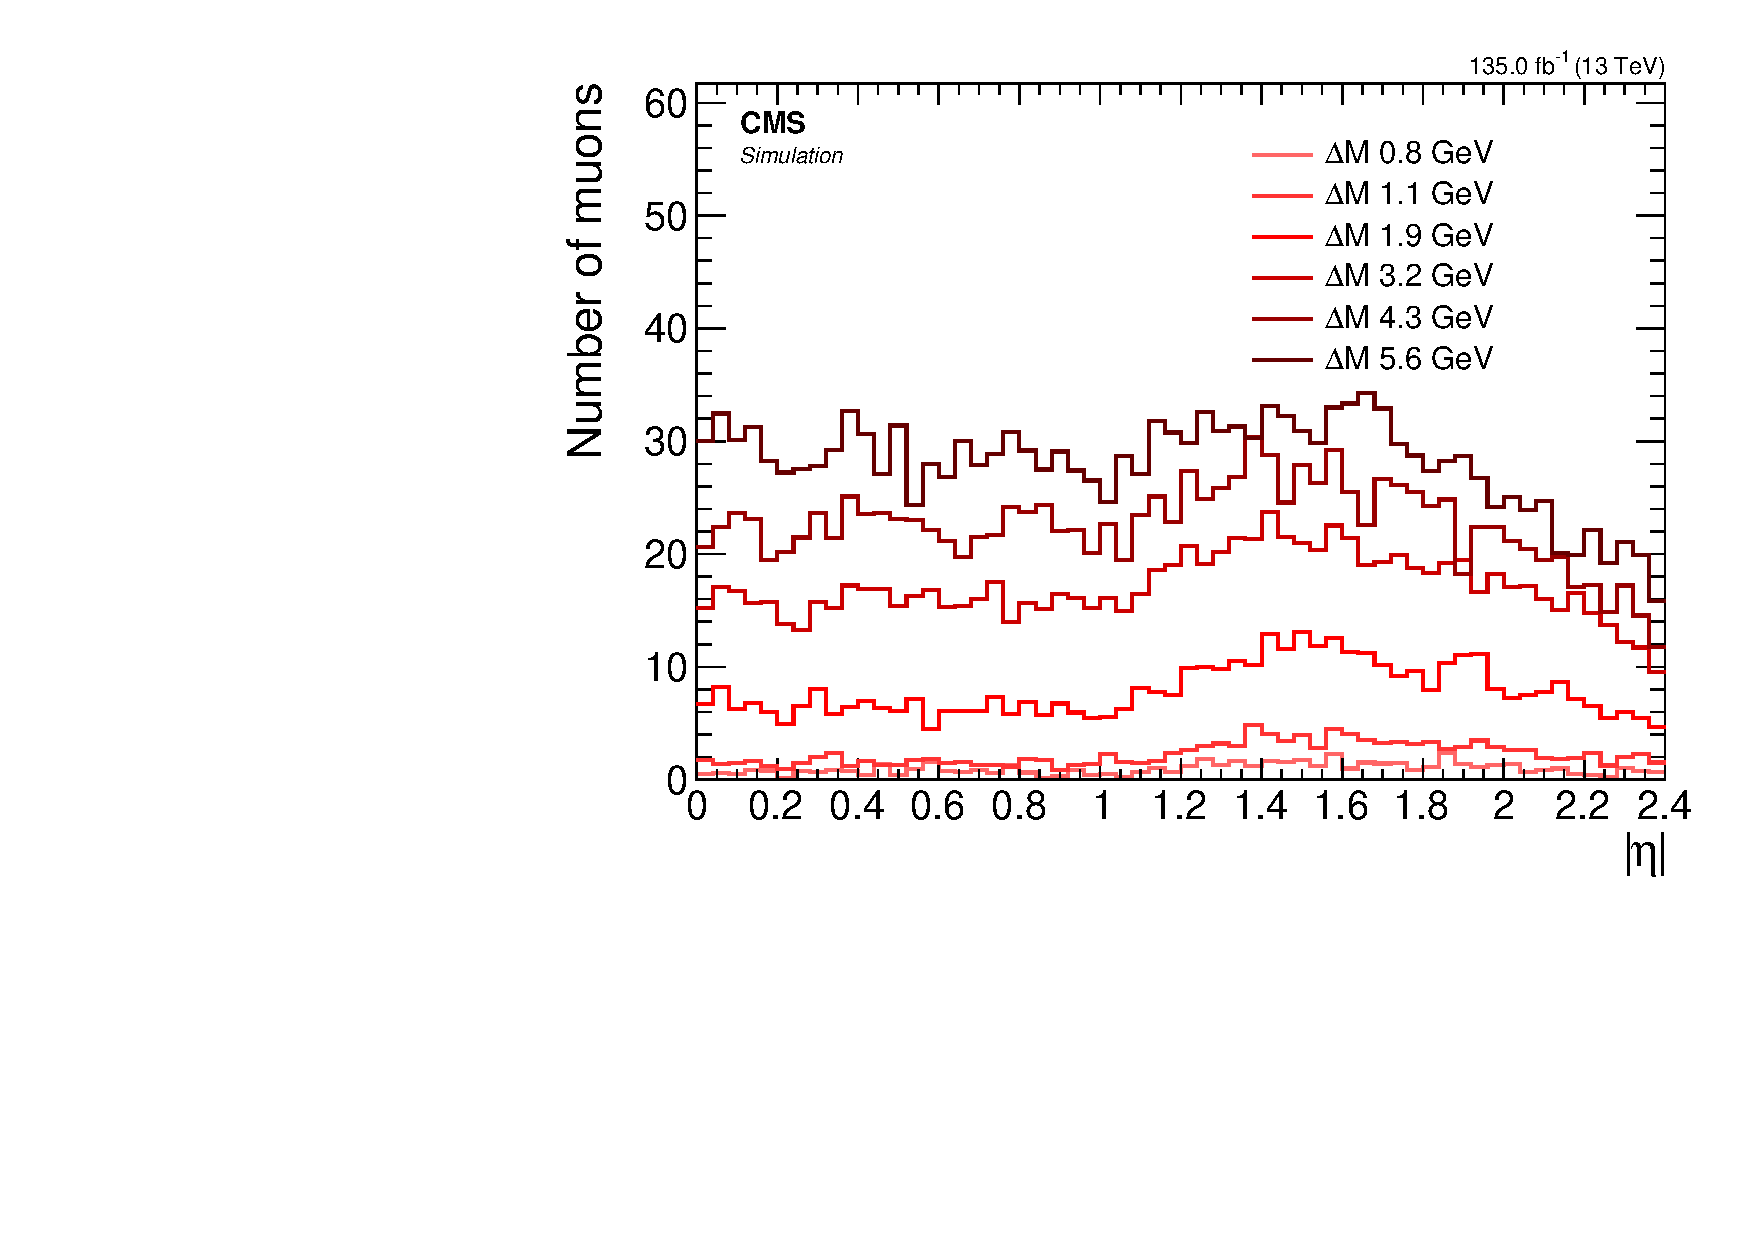
\includegraphics[width=0.32\linewidth]{plots/signal_muons/none_Muons_Eta.pdf} \,
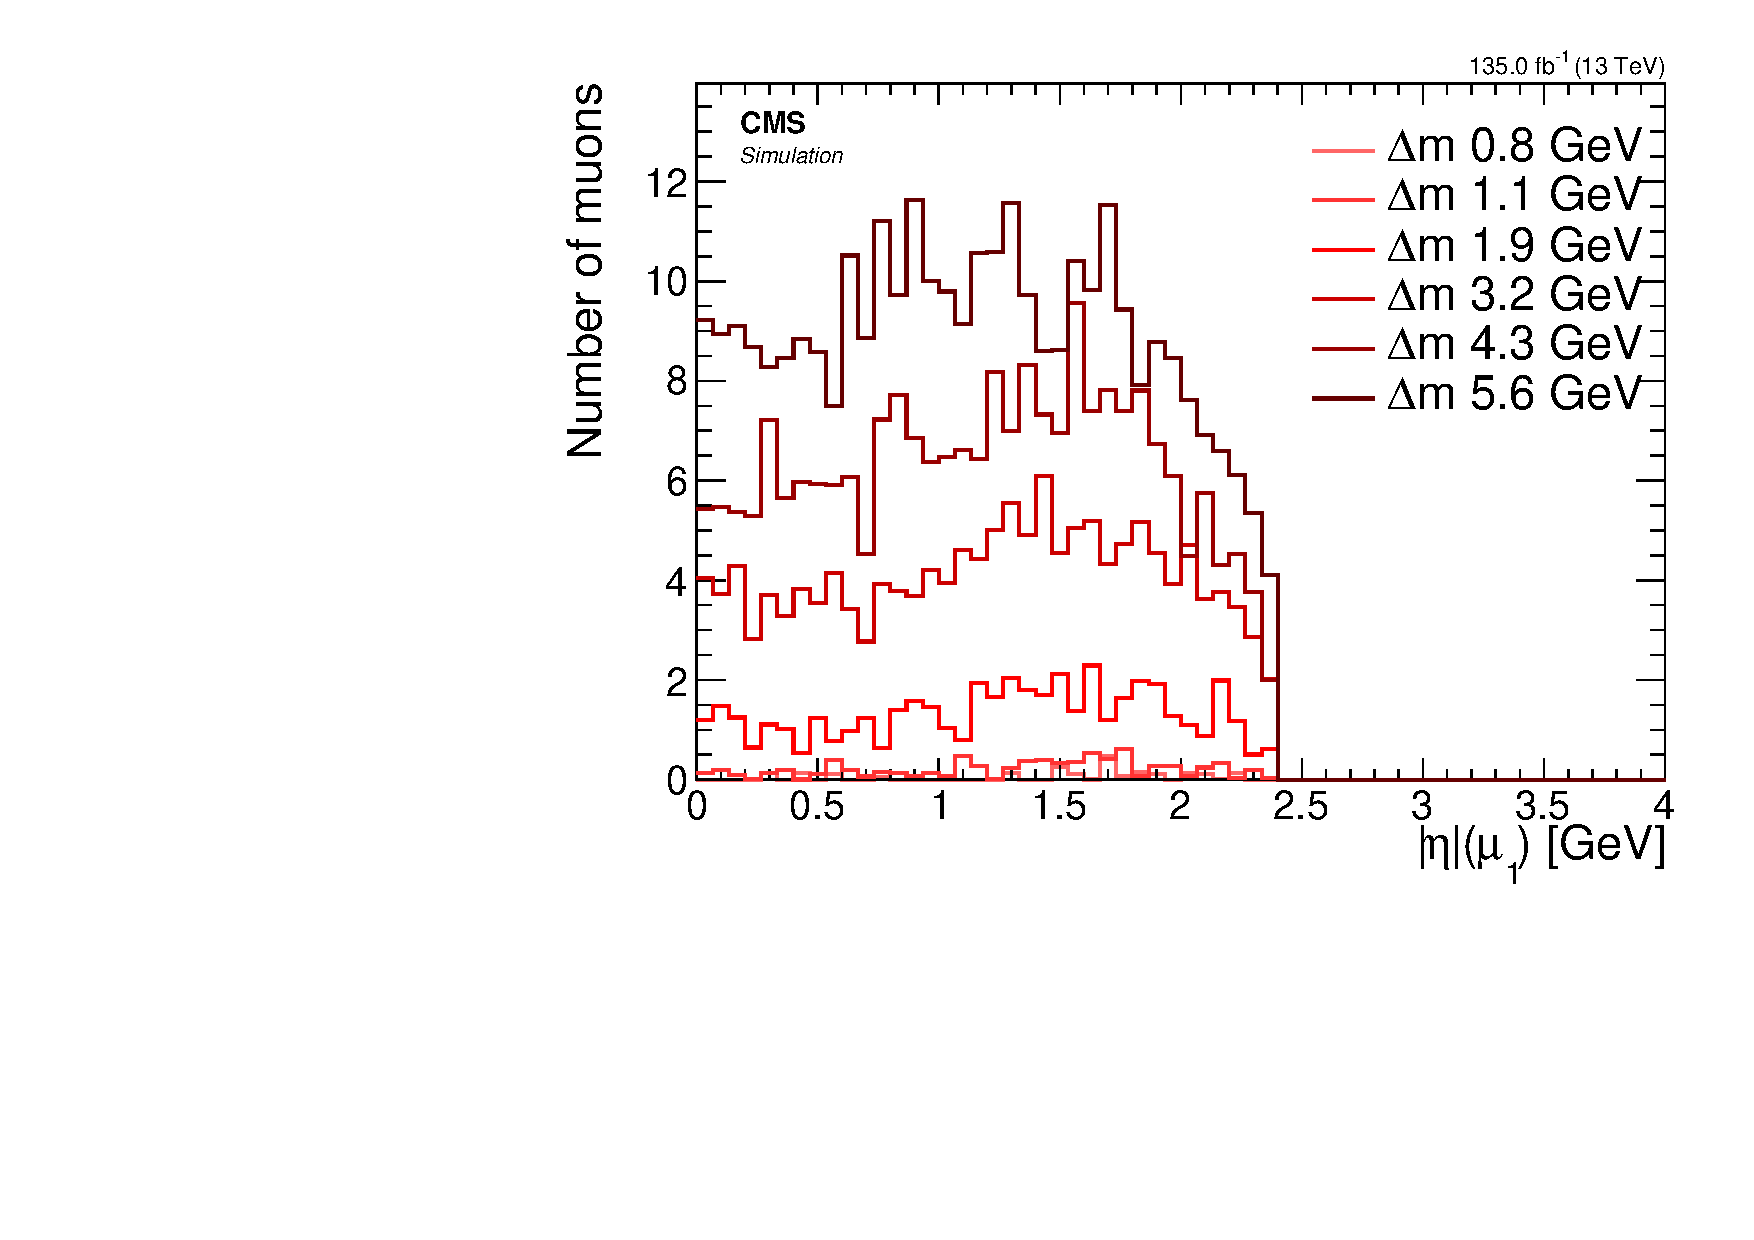
\includegraphics[width=0.32\linewidth]{plots/signal_muons/none_Muons_m1_eta.pdf}  \,
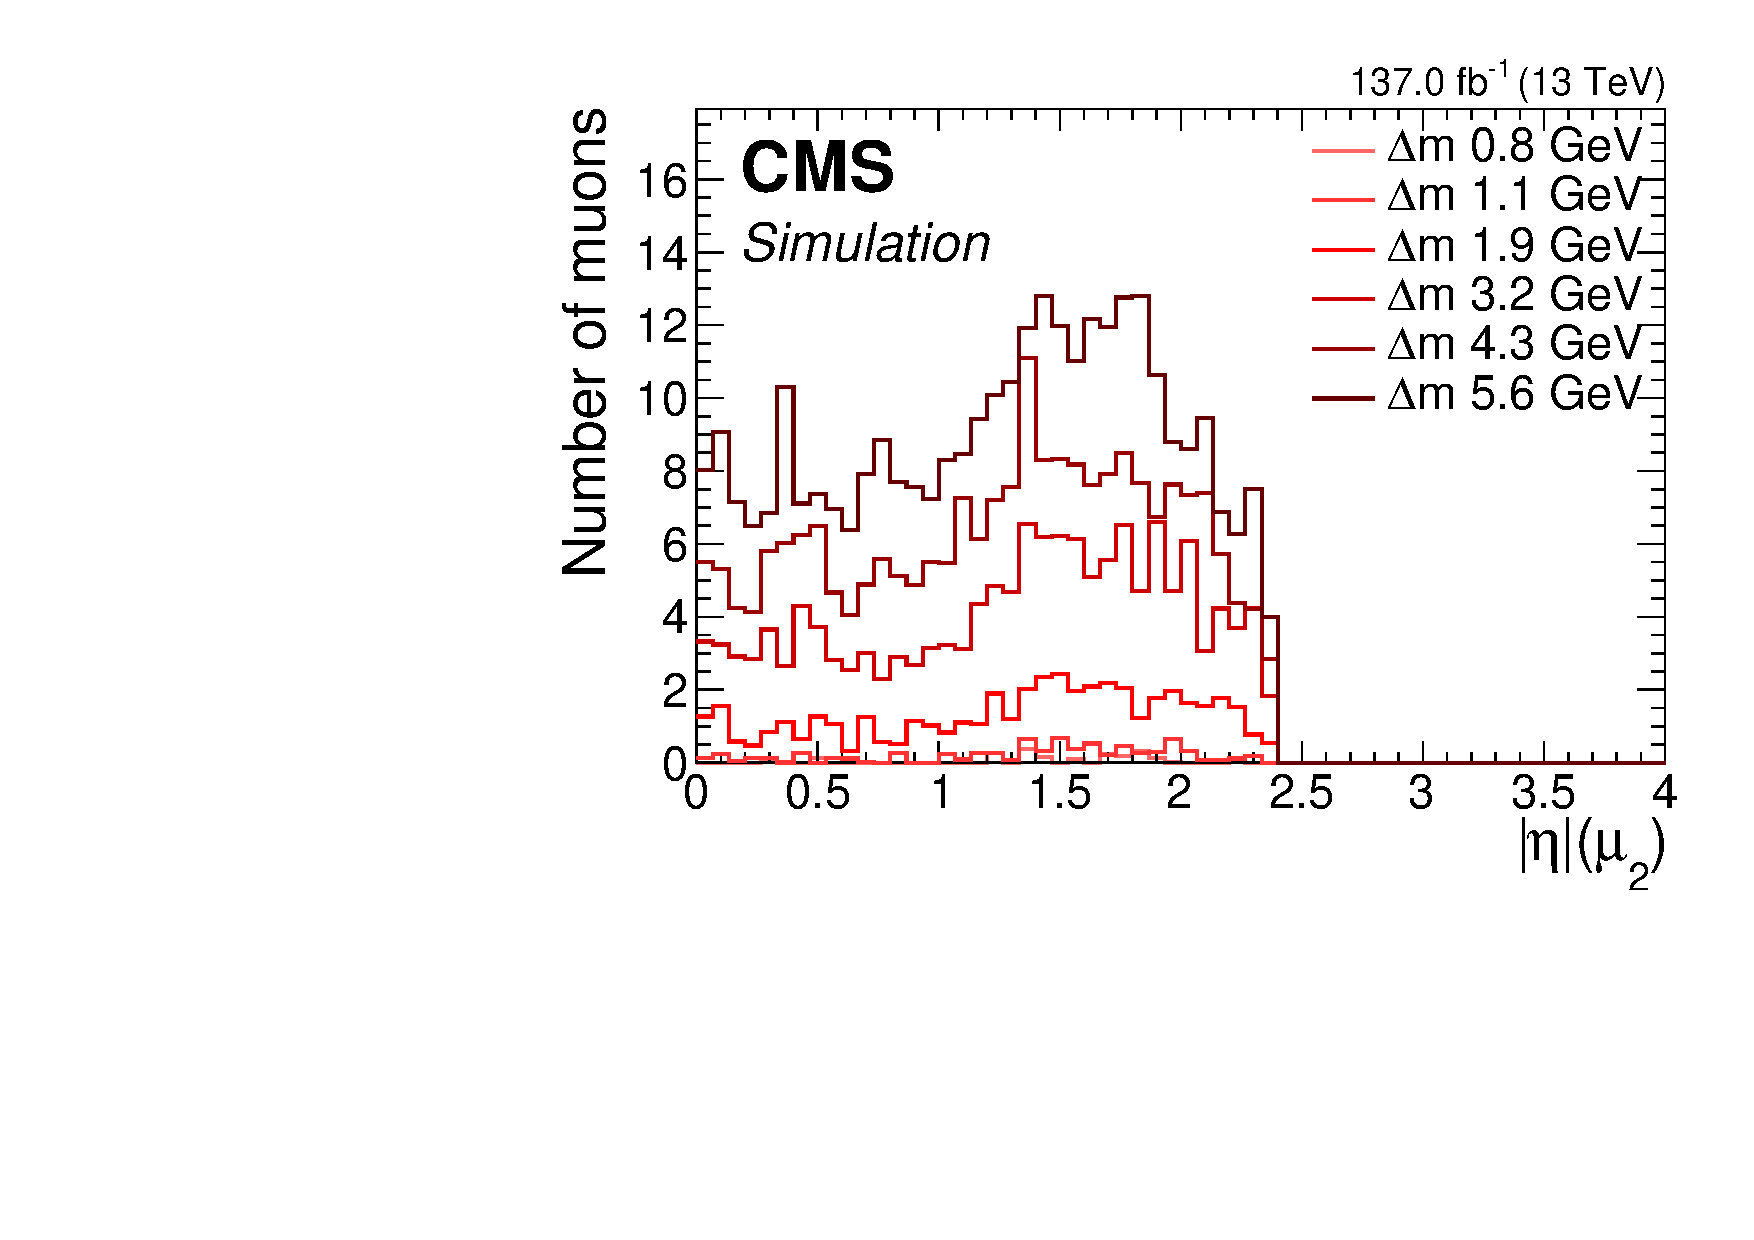
\includegraphics[width=0.32\linewidth]{plots/signal_muons/none_Muons_m2_eta.pdf} \\
\caption[Signal $\abs{\eta}$ distributions]{ Signal $\abs{\eta}$ distributions for inclusive (left), leading muon $\mu_1$ (middle),  subleading muon $\mu_2$ (right) at generator level (top) and reconstruction level passing analysis selection (bottom). }
\label{fig:signal-muons-eta}
\end{figure}

Our muons analysis selection picks only muons in the tracker range of $\abs{\eta}<2.4$ which is the reason why the reconstruction plots on the bottom do not have muons with $\abs{eta}>2.4$. We see that the main effect going from the inclusive $\abs{\eta}$ in generator level to the reconstructed counter part, is the flattening of the distribution due to the loss of muons with $\abs{eta}<1.2$ in the barrel for muons with $\pt<3\GeV$.

With the understanding of the reconstruction effects on the \pt and $\eta$ distributions of the muons, we are equipped to look further into other kinematic variables of the dilepton system.

\subsubsection{Invariant mass \gls{mll}}
\label{sec:gen-invariant-mass}

The invariant mass of the two leptons that result from the decay of the \neutt has a unique shape due to the limited allowed phase space of the leptons as part of the 3-body decay. Since the \neutt decays into \neuto and \ellell through a \PZstar, the allowed phase space of the dilepton pair is restricted to the mass difference between \neutt and \neuto, \ie, \dm. We therefore expect the \gls{mll} distribution to have an edge at \dm.

\begin{figure}[!htb]
\centering
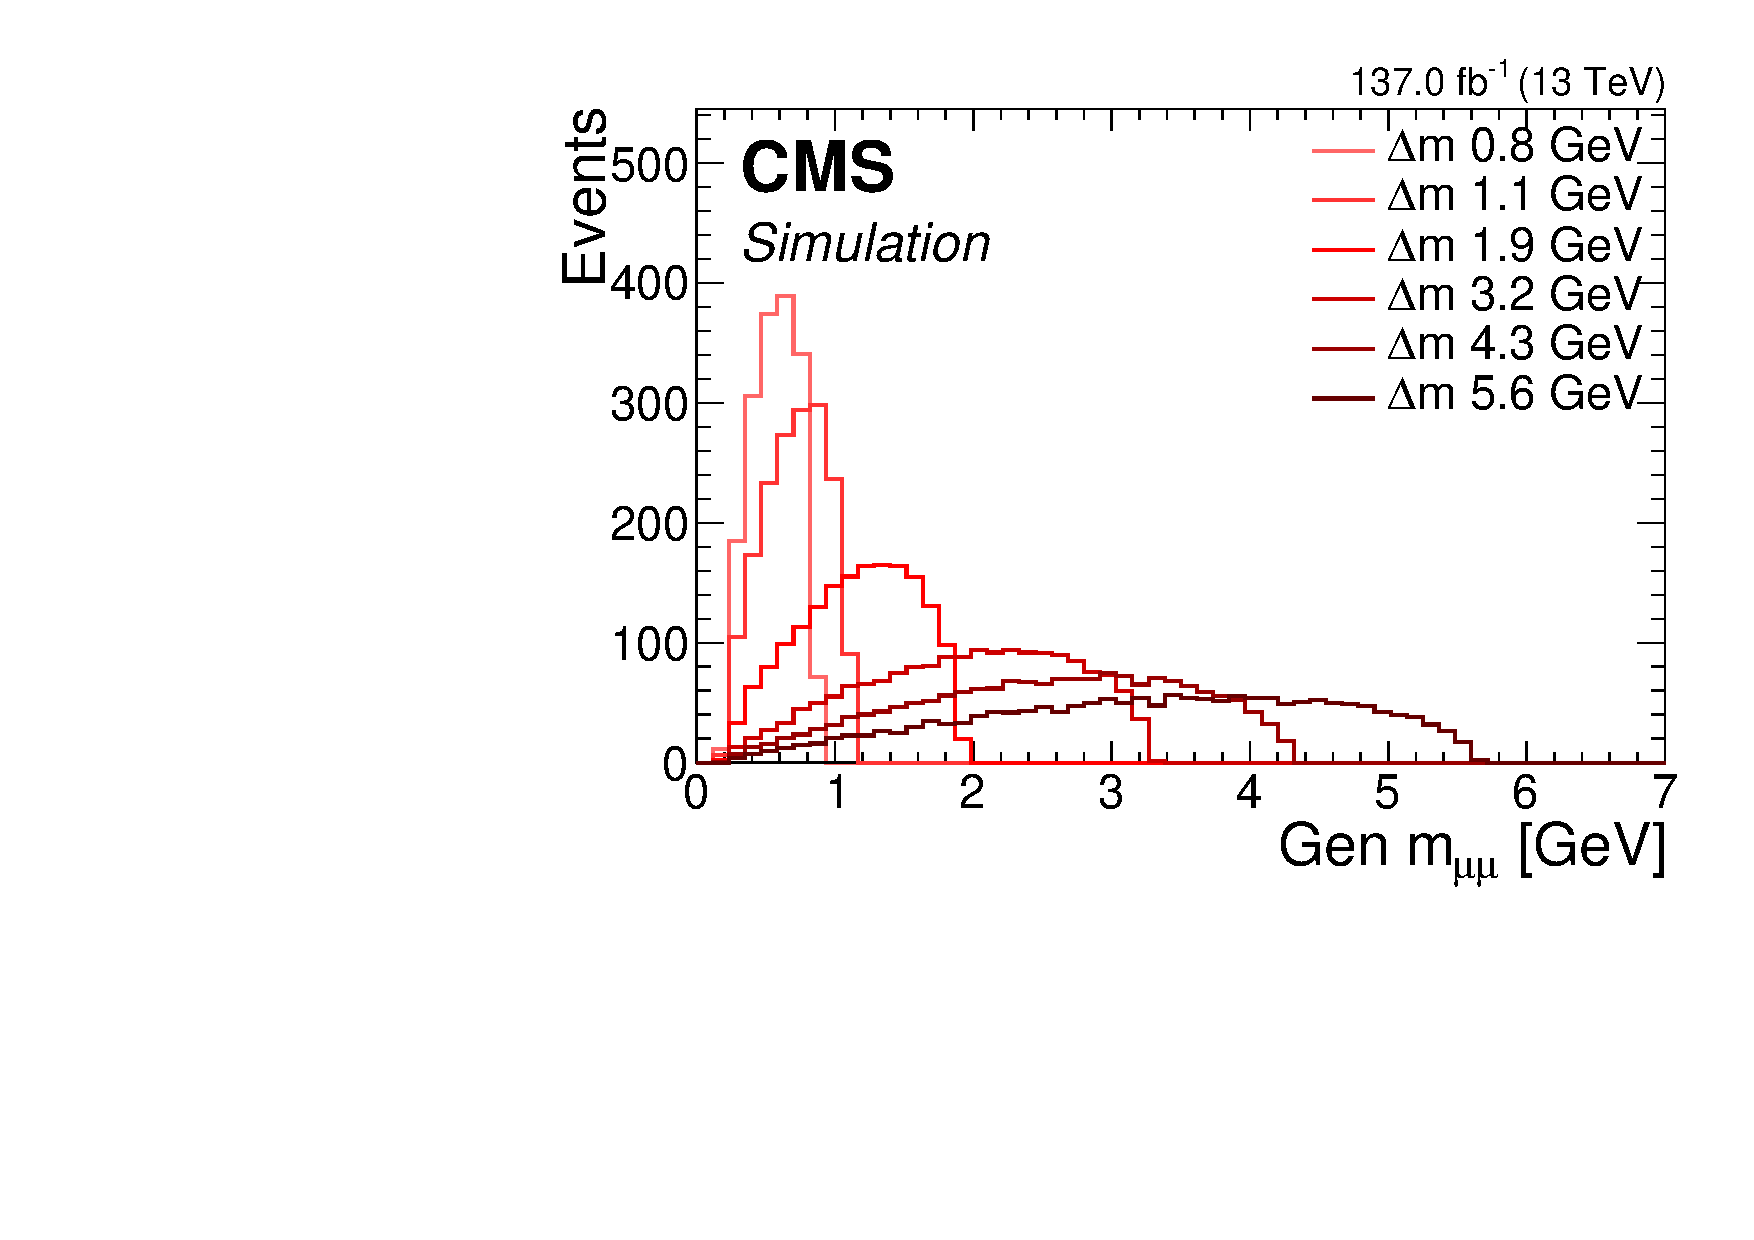
\includegraphics[width=0.32\linewidth]{plots/signal_muons_gen/none_gen_invMass.pdf} \,
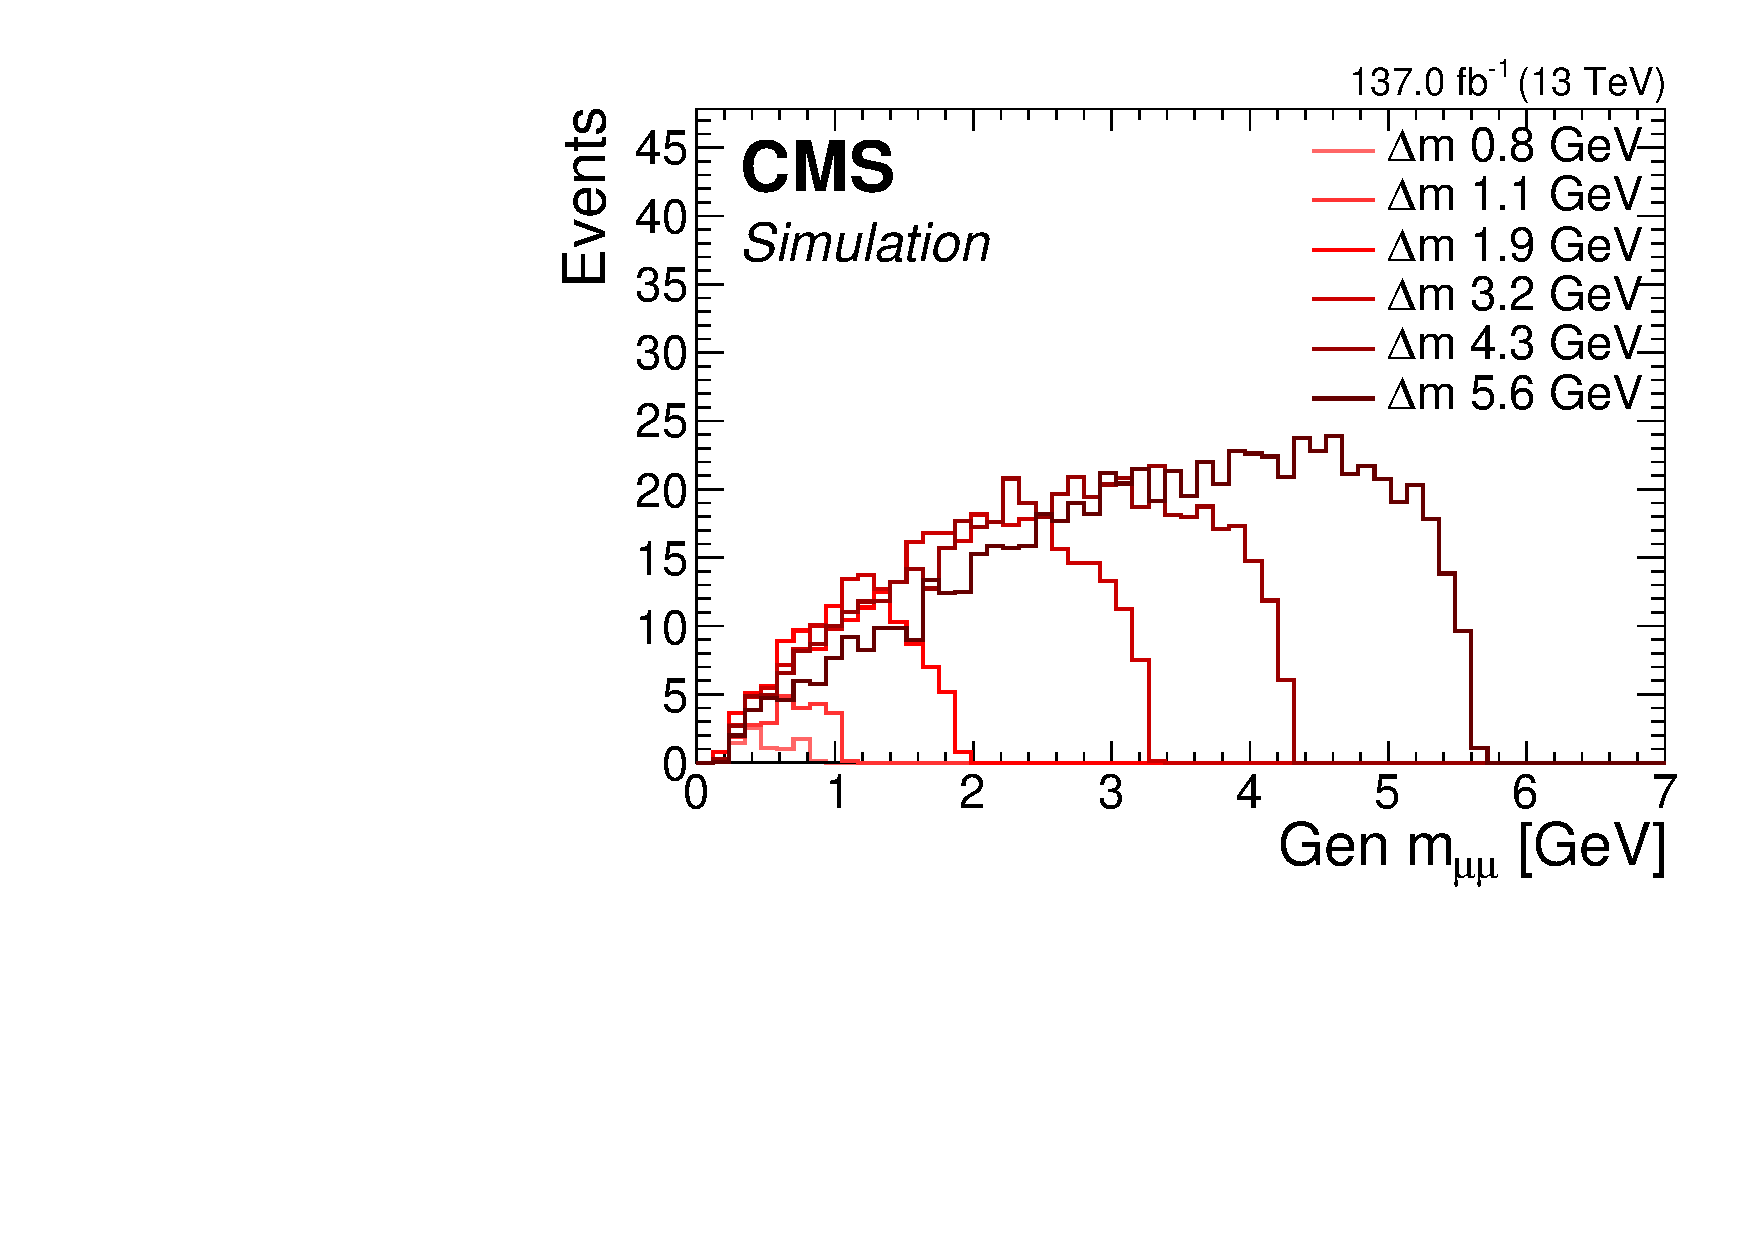
\includegraphics[width=0.32\linewidth]{plots/signal_muons_gen/none_gen_invMass_cut.pdf}  \,
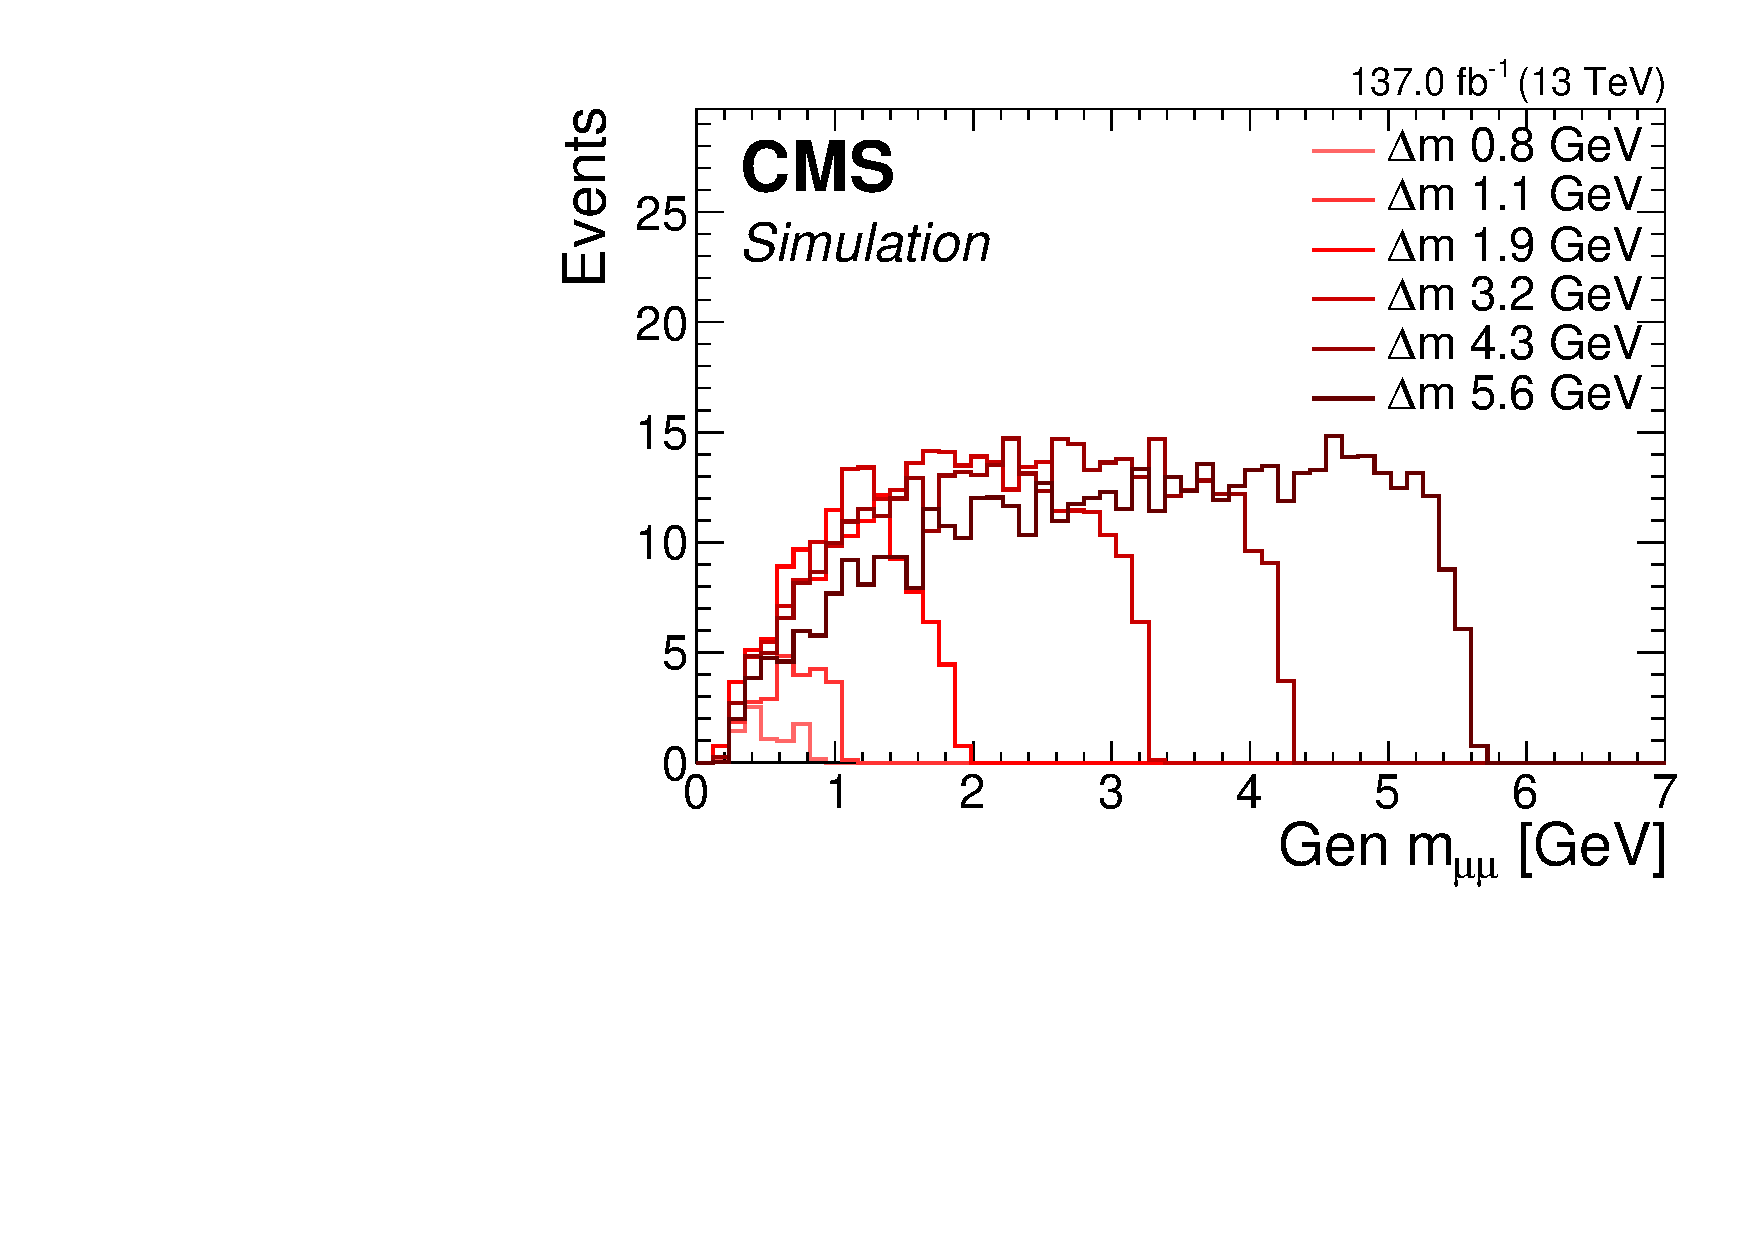
\includegraphics[width=0.32\linewidth]{plots/signal_muons_gen/none_gen_invMass_orth.pdf} \\
\caption[Signal generator level \mll distributions]{ Signal generator level \mll distributions with no cuts (left), with $\pt\left(\mu_i\right)>2\GeV,\,i=1,2$ (middle) and with \gls{sos} orthogonality condition $\pt\left(\mu_i\right)>2\GeV$, $\pt\left(\mu_2\right)\leq~3.5\GeV\text{ or }\Delta R\leq 0.3$ (right).}
\label{fig:signal-generator-mll}
\end{figure}

We see the original invariant mass of the muons \mmumu on the left. For each signal point, the edge of the \mmumu distribution is right at the corresponding \dm. However, once we cut on the muons \pt and require $\pt\geq 2\GeV$, the shape shifts, and the efficiency in the lower \dm drops dramatically, as can be seen from the middle plot. Lastly, the effect of orthogonalizing phase space to the \gls{sos} analysis can be seen on the right most plot. The effect is strongest in high \dm and quite subtle in low \dm. 

To understand the reshaping that happens to the \mmumu shape, we look at the relationship between the \pt of the muons (leading muon denoted $\mu_1$ while subleading muon is denoted $\mu_2$) and the invariant mass one a signal with low \dm of $1.13\GeV$ and one with high \dm of $5.63\GeV$.

\begin{figure}[!htb]
\centering
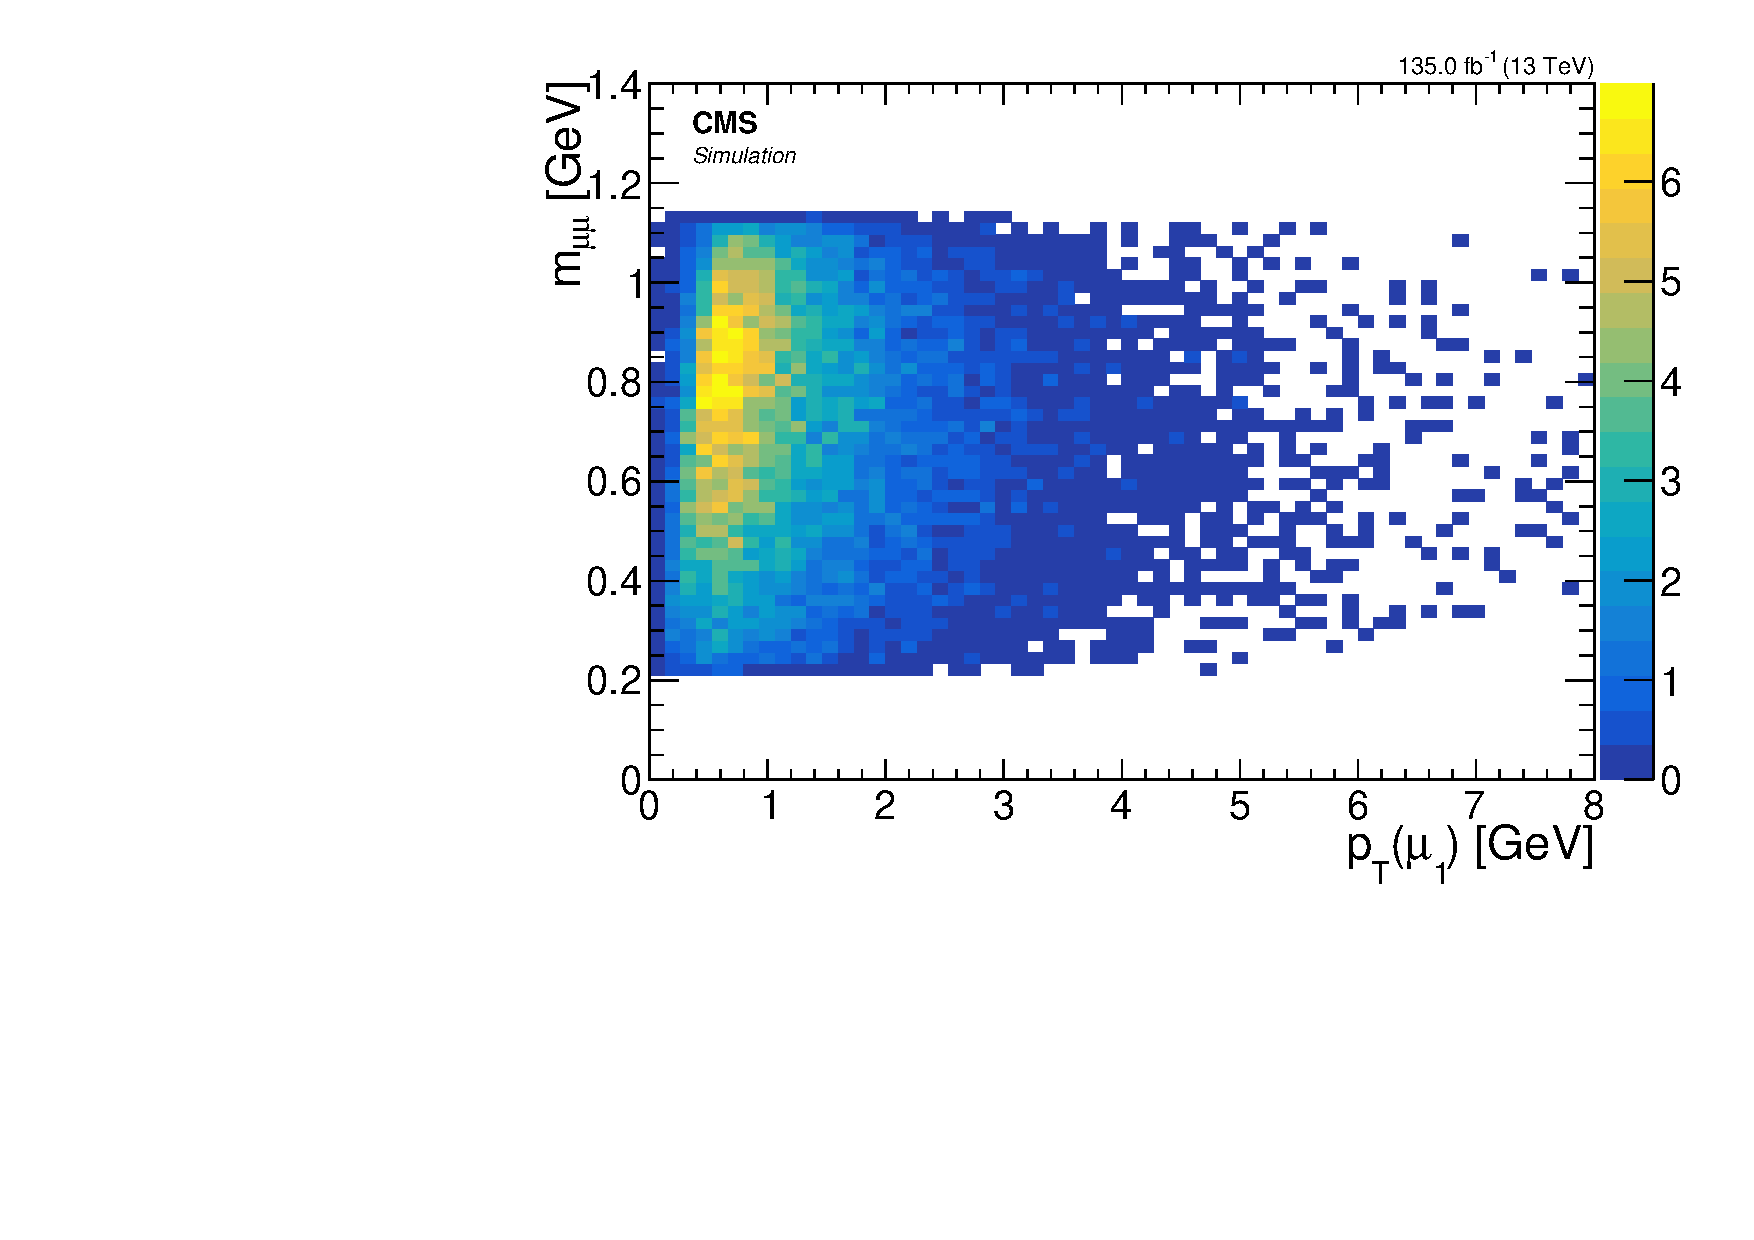
\includegraphics[width=0.48\linewidth]{plots/signal_muons_gen_delta_r_vs_pt/none_gen_invmass_vs_pt_1.pdf} \,
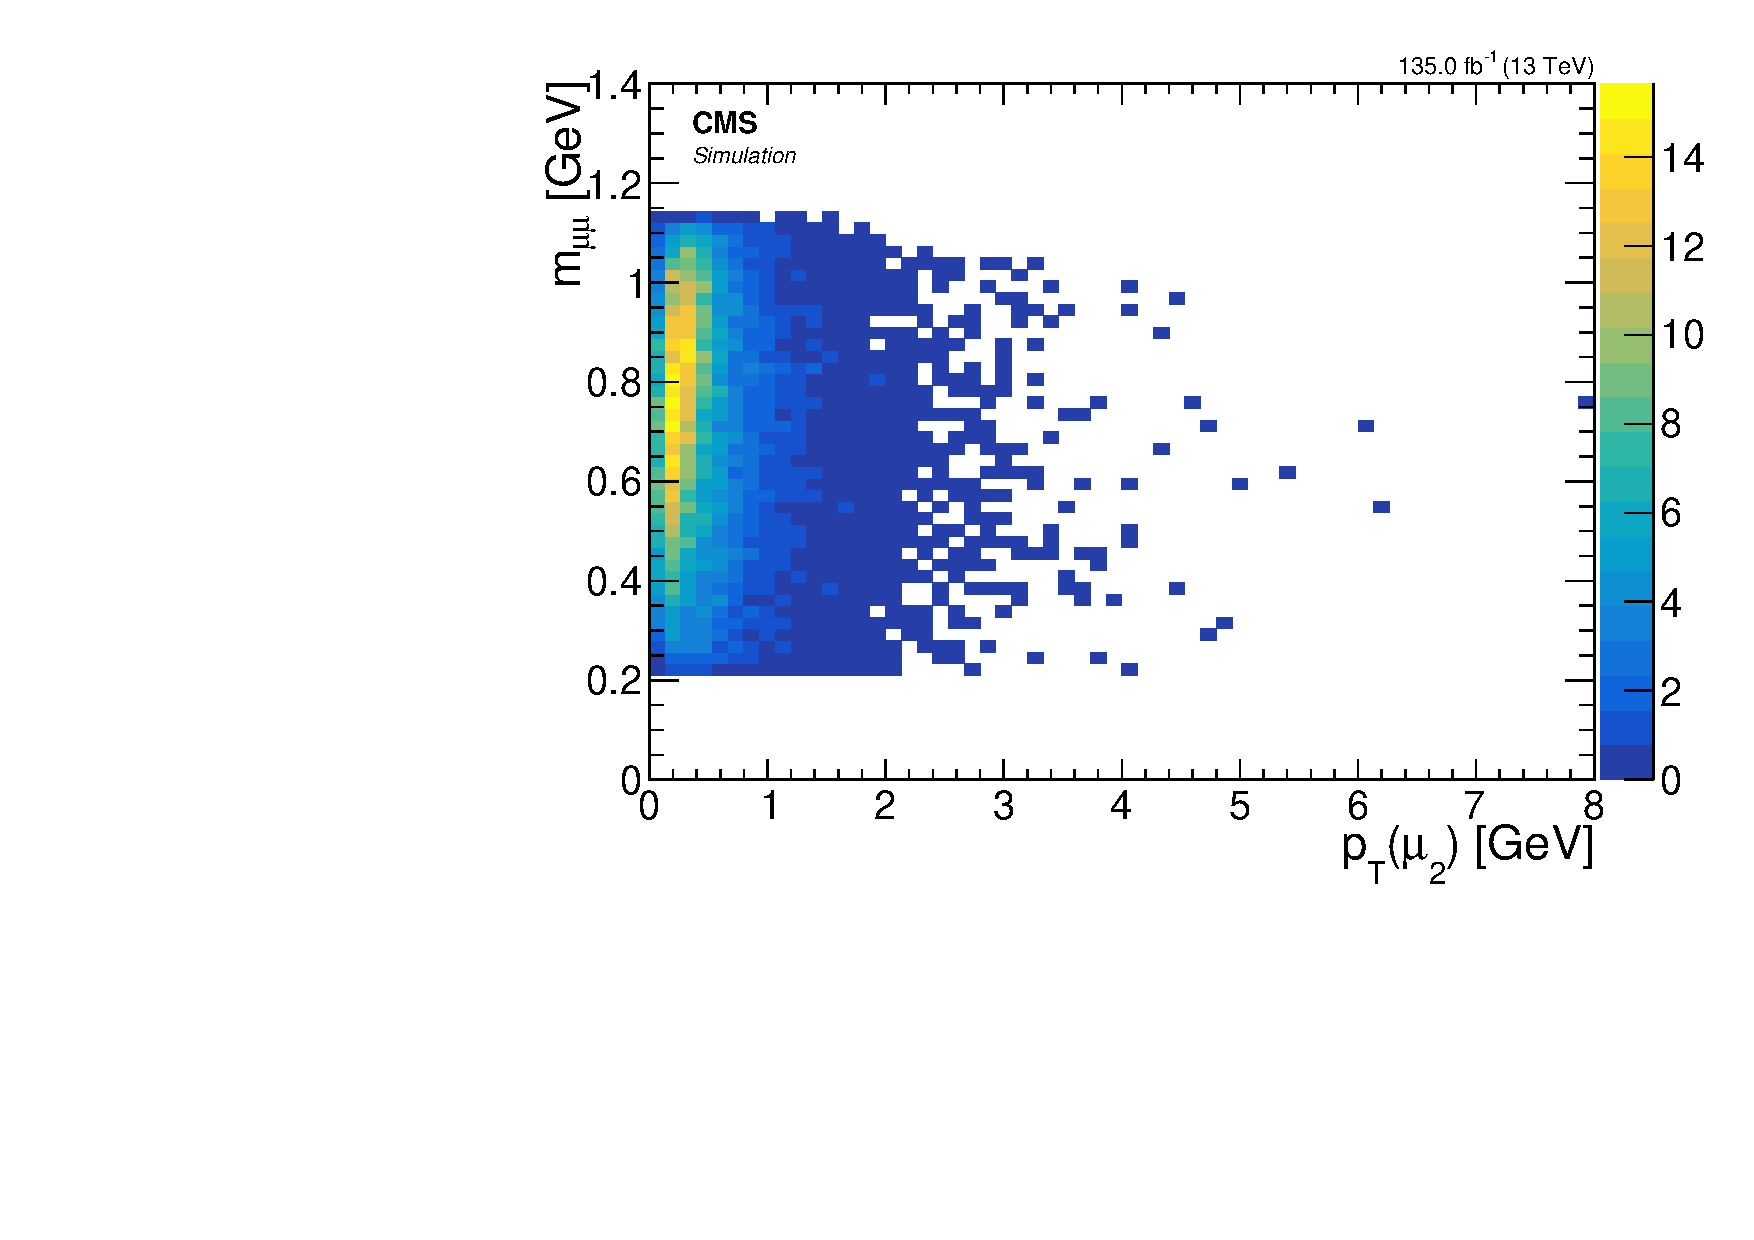
\includegraphics[width=0.48\linewidth]{plots/signal_muons_gen_delta_r_vs_pt/none_gen_invmass_vs_pt_2.pdf}  \\
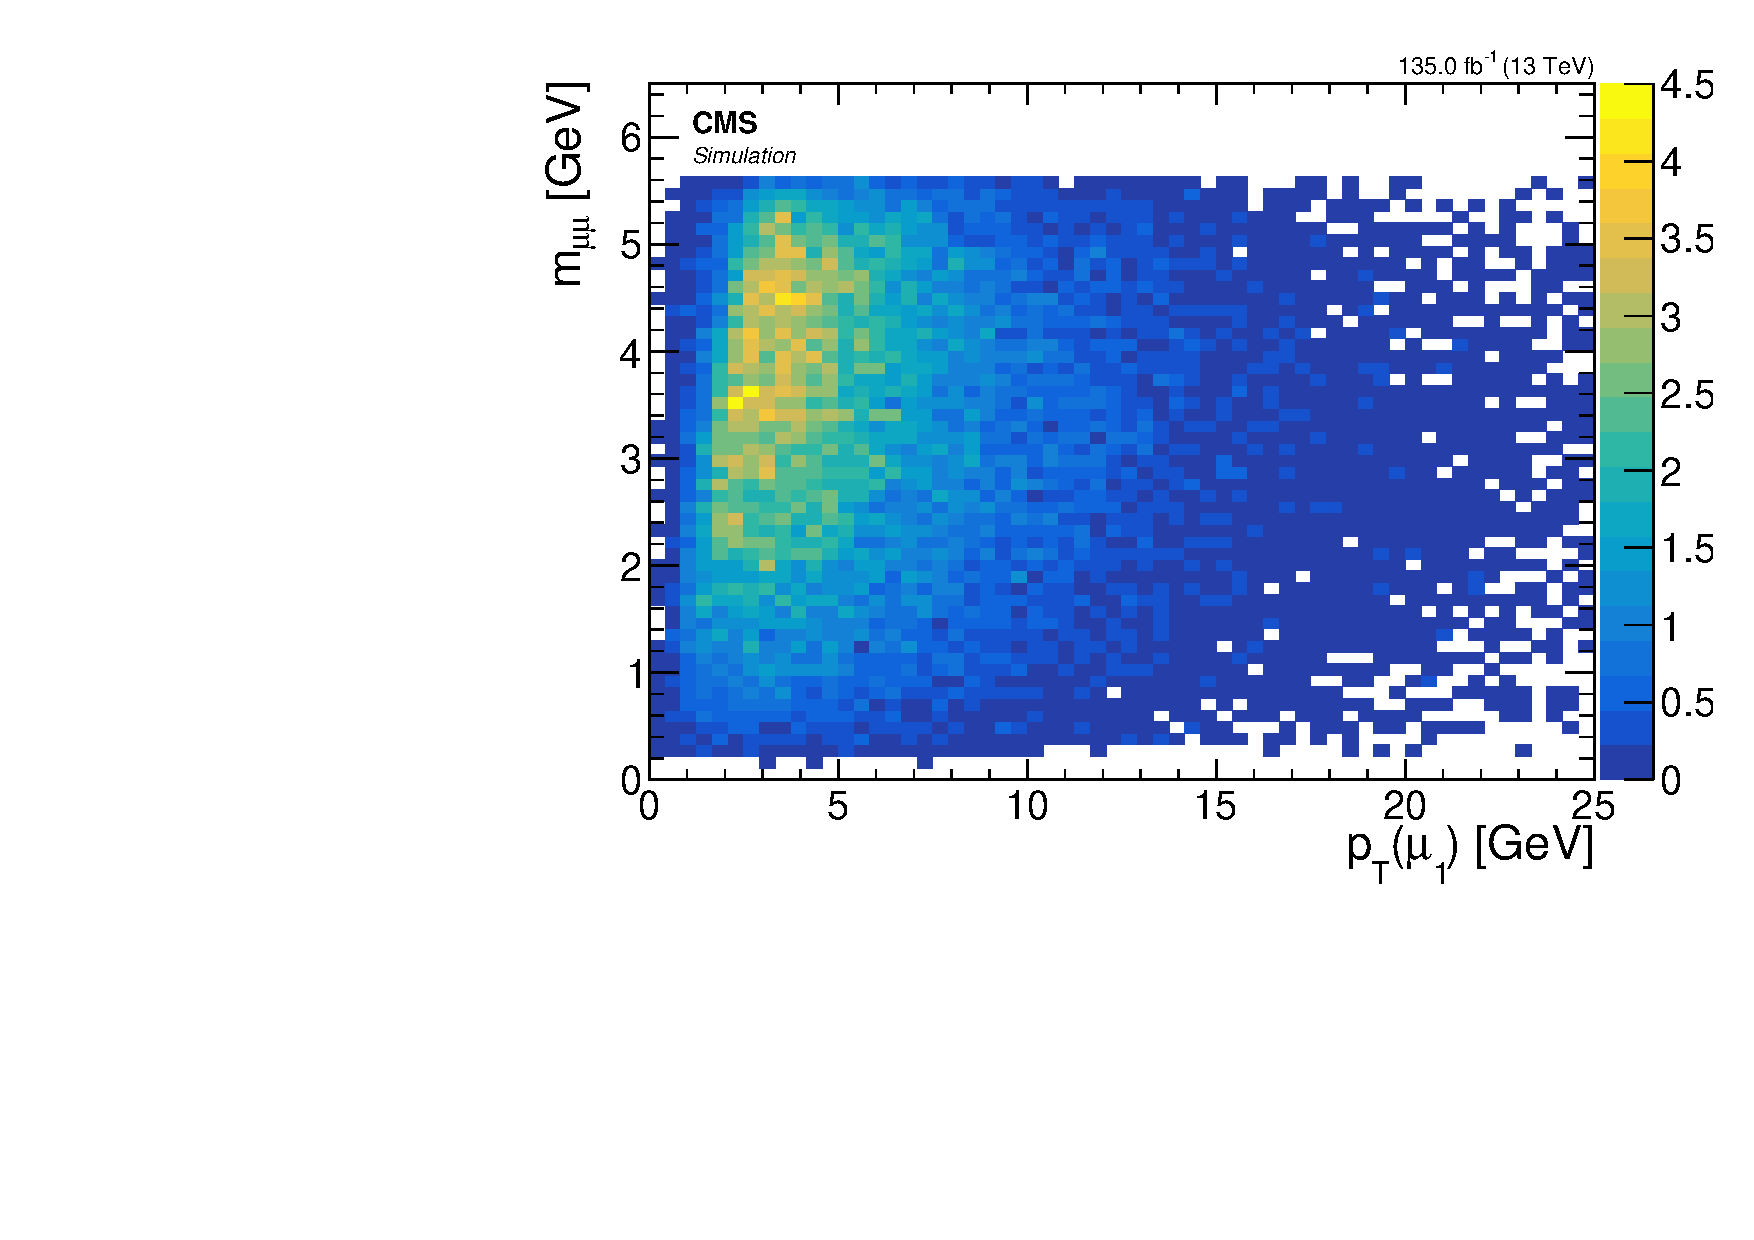
\includegraphics[width=0.48\linewidth]{plots/signal_muons_gen_delta_r_vs_pt_dm5/none_gen_invmass_vs_pt_1.pdf} \,
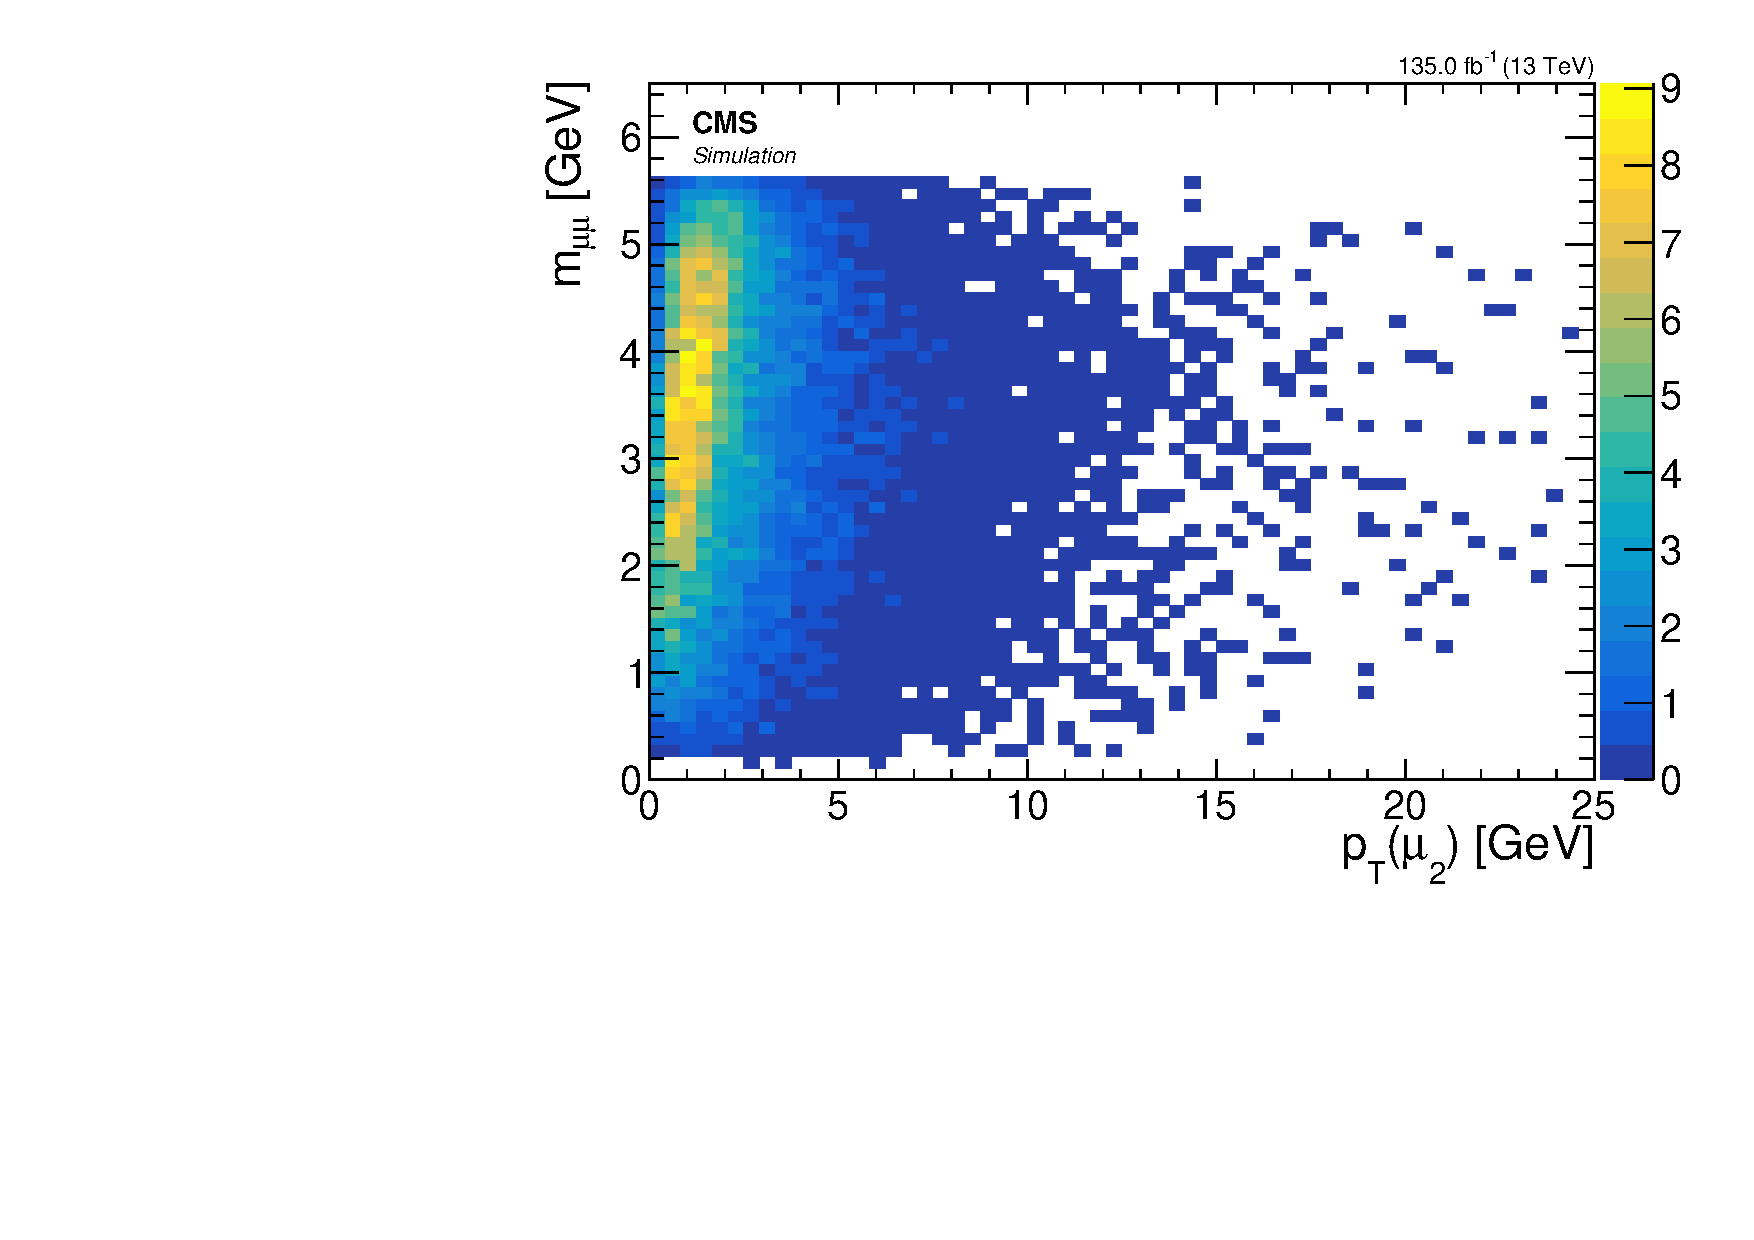
\includegraphics[width=0.48\linewidth]{plots/signal_muons_gen_delta_r_vs_pt_dm5/none_gen_invmass_vs_pt_2.pdf}  \\
\caption[Signal \mmumu \vs \pt]{ Signal \mmumu \vs \pt for leading lepton $\mu_1$ (left) and subleading lepton $\mu_2$ (right) for $\dm=1.13\GeV$ (top) and $\dm=5.63\GeV$ (bottom).}
\label{fig:signal-gen-invamass-pt}
\end{figure}

We have established earlier that the invariant mass distribution has an edge at the \dm and one can read the value of \dm from these plots. Another interesting feature to notice in these plots is that there is also a lower edge in the \dm distribution at around $\sim 0.2\GeV$ and that is of course due to each muon having a mass of around $\sim 0.1\GeV$. We can clearly see now that by cutting on both muons at $\pt\geq 2\GeV$, we are loosing a lot of the signal. This effect, in fact, becomes quite substantial for the low $\dm=1.13\GeV$ (top row). We quantify this effect by making a cutflow table where each row represents a cut, and its efficiency is calculated by dividing the number of events passing the cut by the number of events in the line before it. The first line is our baseline of all dimuon events with at least one jet with $\pt \geq 30\GeV$ and $\abs{\eta}<2.4$ and has an efficiency of 1 by definition. The event number is weighted to Run II luminosity of $\lumi = 135 \fbinv$.

\begin{table}[!htb]
	\centering
	\label{tab:gen-muon-pt-dr-efficiency}
		\caption{Generator level efficiency on muons selections}
		%\vspace{1mm}
			\begin{tabular}{l|cc|cc} \hline
			Cut & \multicolumn{2}{c|}{Number of events} & \multicolumn{2}{c}{Efficiency} \\ \hline
			
			 & $\dm=1.13\GeV$ & $\dm=5.63\GeV$ & $\dm=1.13\GeV$ & $\dm=5.63\GeV$ \\
			Baseline & 1710.7 & 1743.9 & 1 & 1\\
			$\pt\geq 2\GeV$ & 24.7 & 724.9 & 0.015 & 0.41\\
			\gls{sos} orthogonality & 24.7 & 490.6 & 1 & 0.68 \\ \hline
			\end{tabular}
\end{table}

We observe that for the low \dm of $1.13\GeV$ the cut of $\pt\geq 2\GeV$ is really hurting the acceptance of the signal with only $1.5\%$ of signal remaining. In contrast, the orthogonality condition of requiring $\pt\left(\mu_2\right)\leq~3.5\GeV\text{ or }\drll\leq 0.3$ is not effecting it any further. The picture is different for the high \dm of $5.63\GeV$ where the \pt cut is cutting away more than half of the signal and the \gls{sos} orthogonality an additional two thirds.

Since we have just established that due to the relationship between \pt and \mll, the \pt distribution directly effects \mll, we should also have a look at how to reconstruction effects discussed at~\ref{sec:muon-eta-pt} might effect the \mmumu distribution as well.

\begin{figure}[!htb]
\centering
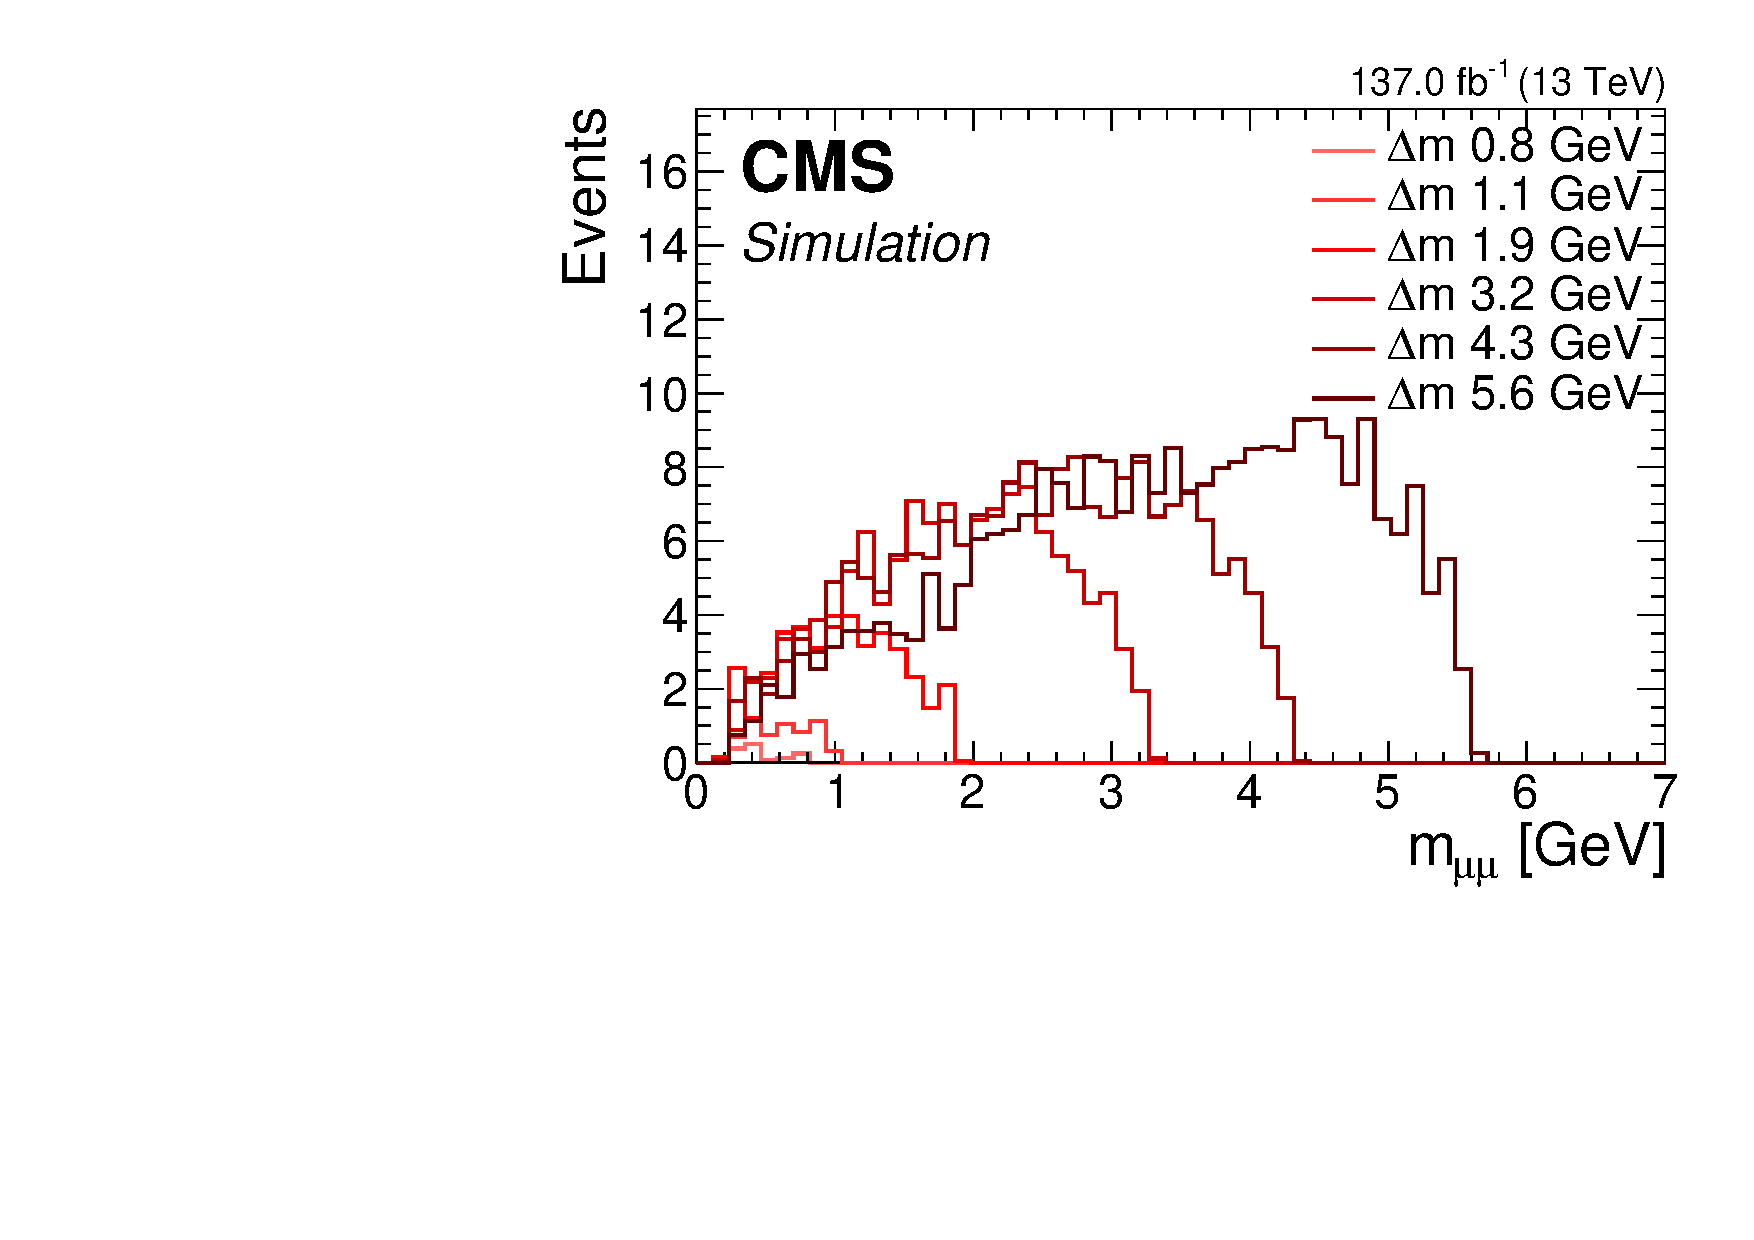
\includegraphics[width=0.48\linewidth]{plots/signal_muons/none_invMassCorrJetNoMultIso10Dr0.6.pdf} \,
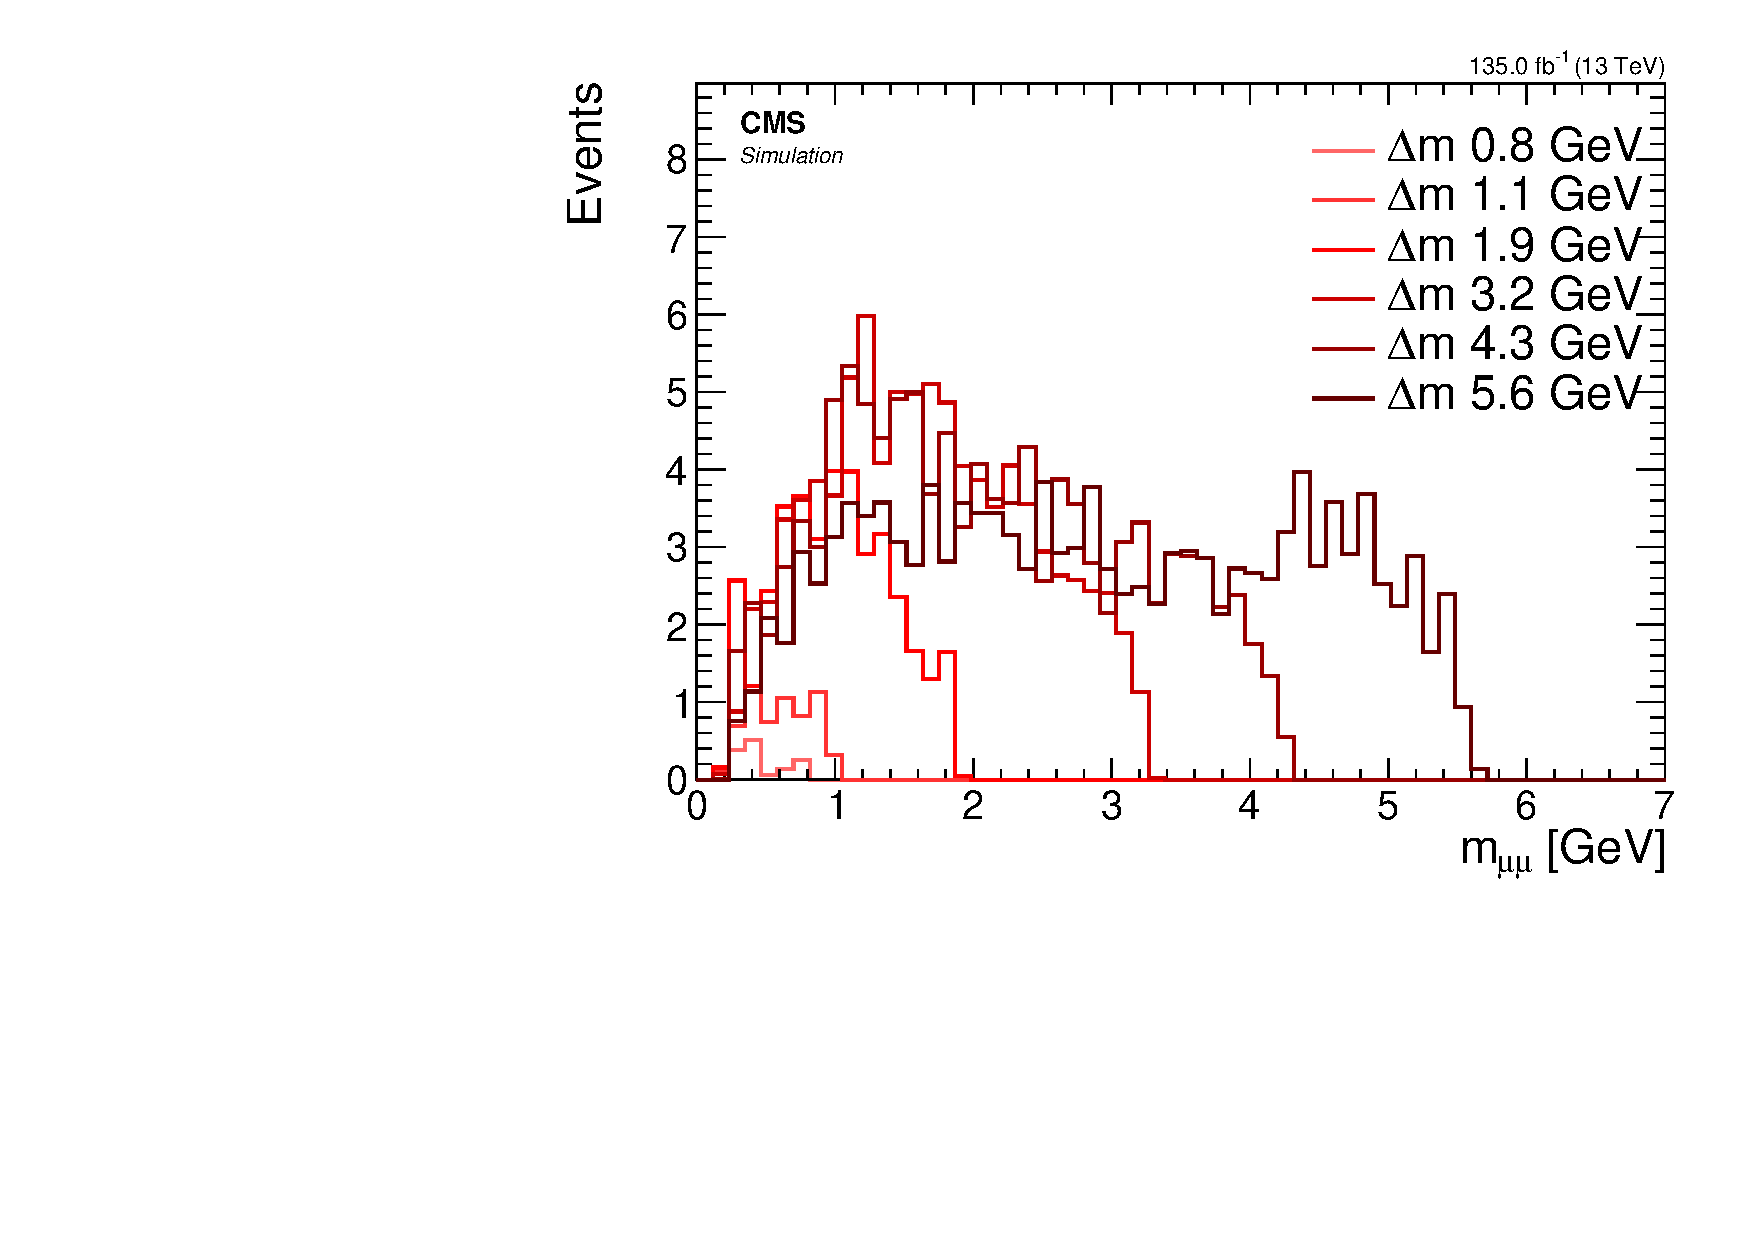
\includegraphics[width=0.48\linewidth]{plots/signal_muons/none_invMassCorrJetNoMultIso10Dr0.6_orth.pdf}  \\
\caption[Signal reconstructed \mmumu]{ Signal reconstructed \mmumu with basic analysis selection (left) and additional \gls{sos} orthogonality condition (right).}
\label{fig:reco-signal-invamass}
\end{figure}

It's interesting to compare these distributions to the two right ones in the generator level version at \ref{fig:signal-generator-mll}. We see that not only less events survive the reconstruction, but also that some \dm model points peak between $1 \GeV$ to $2 \GeV$ with \gls{sos} orthogonality condition applied. The reconstruction and selection efficiency is discussed in more details in \fxnote{ref}.

\subsubsection{Lepton separation \gls{dr}}
\label{sec:lepton-dr}

The lepton separation is defined by $\DR=\sqrt{\left(\deta\right)^2+\left(\dphi\right)^2}$ where \gls{eta} is the pseudorapidity and \gls{phi} is the azimuthal angle measured in radians. \gls{dr} plays a major role in this analysis since the leptons tend to be produced in proximity to each other and thus to defy standard definitions of isolation. Special care is taken to ensure that the collimated nature of the leptons can still be used to distinguish the otherwise isolated leptons in the signal from the non-isolated leptons in the \gls{sm} background. An additional point of interest is with respect to previous \gls{sos} analysis \fxnote{cite} that had a requirement of $\drll > 0.3$ which we attempt to revert here for orthogonality purposes. 

In similar fashion to the invariant mass in~\ref{sec:gen-invariant-mass}, we look at distributions of \gls{dr} for various choices of \dm with different cuts applied, and observe their effect.

\begin{figure}[!htb]
\centering
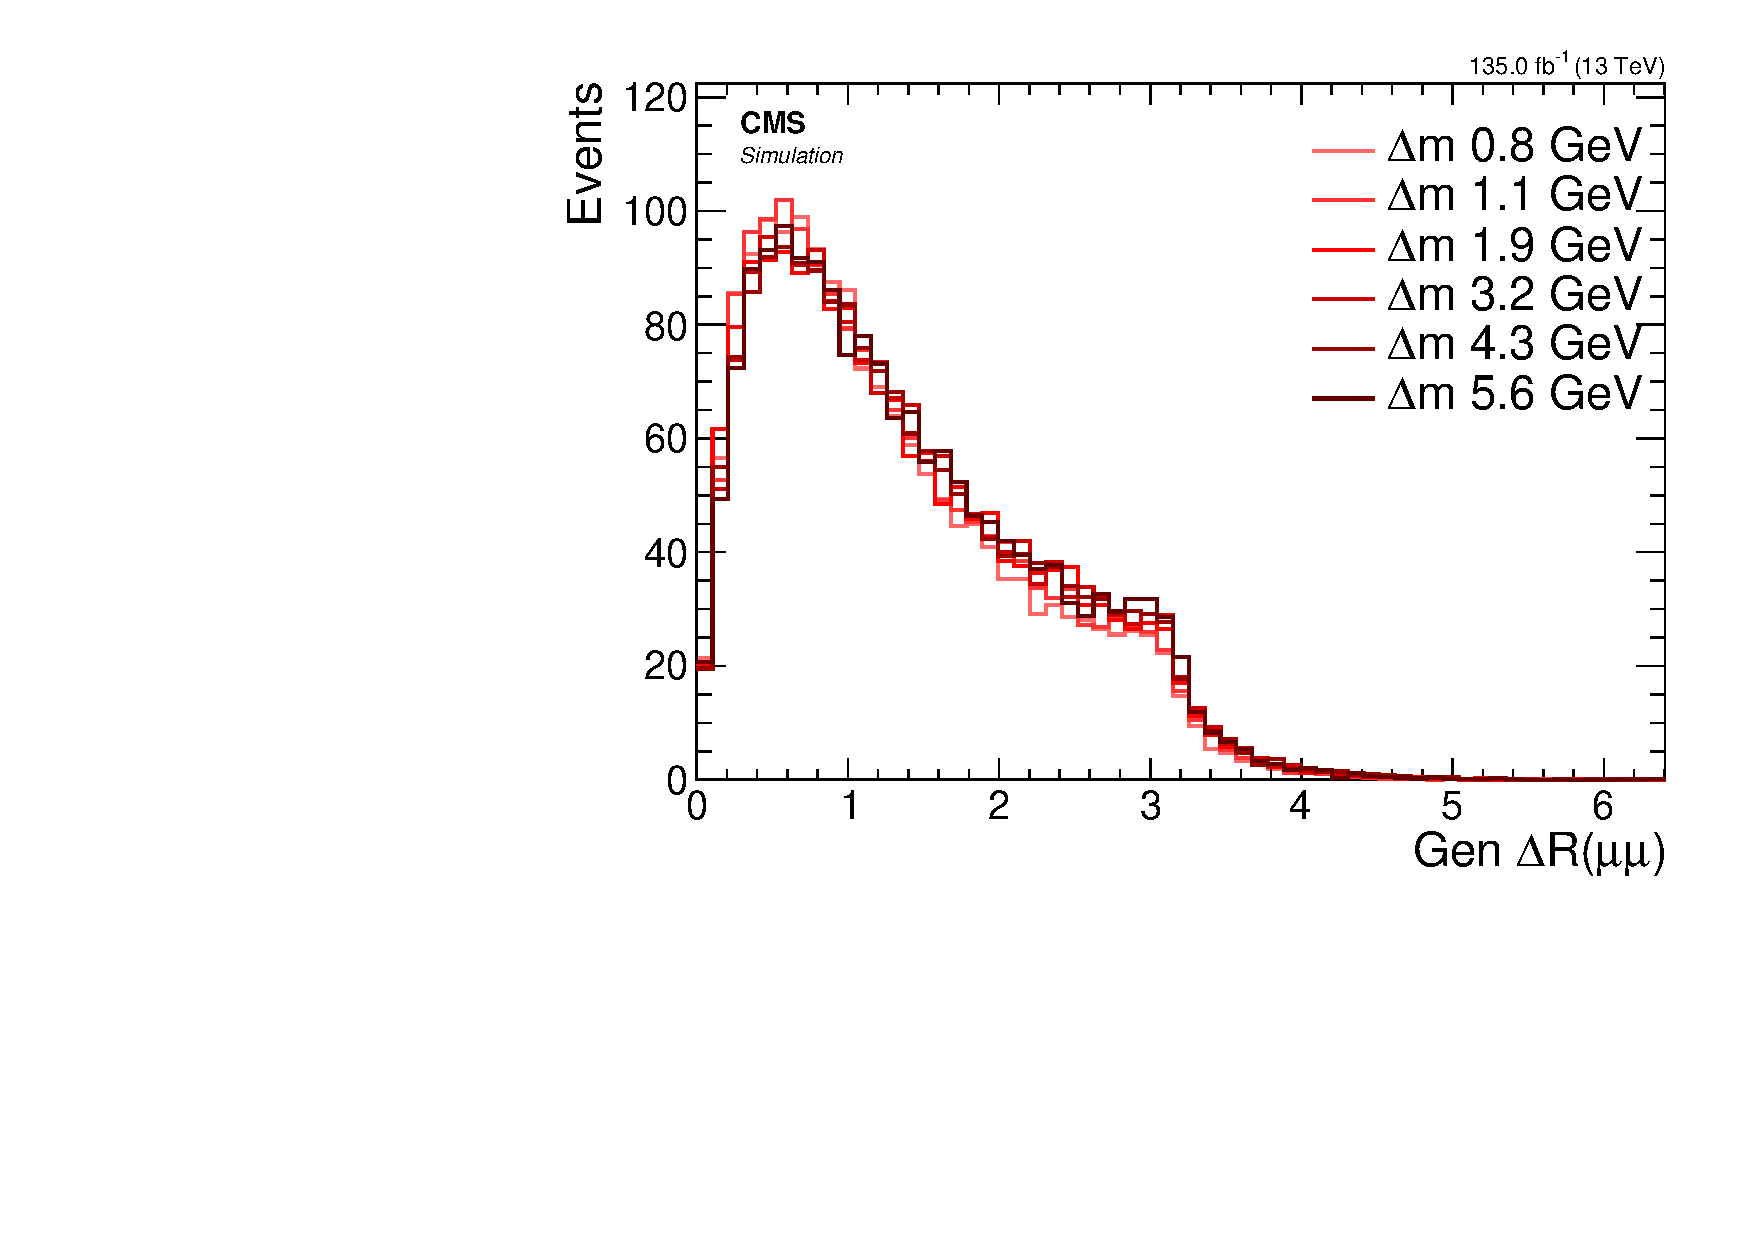
\includegraphics[width=0.32\linewidth]{plots/signal_muons_gen/none_gen_deltaR.pdf} \,
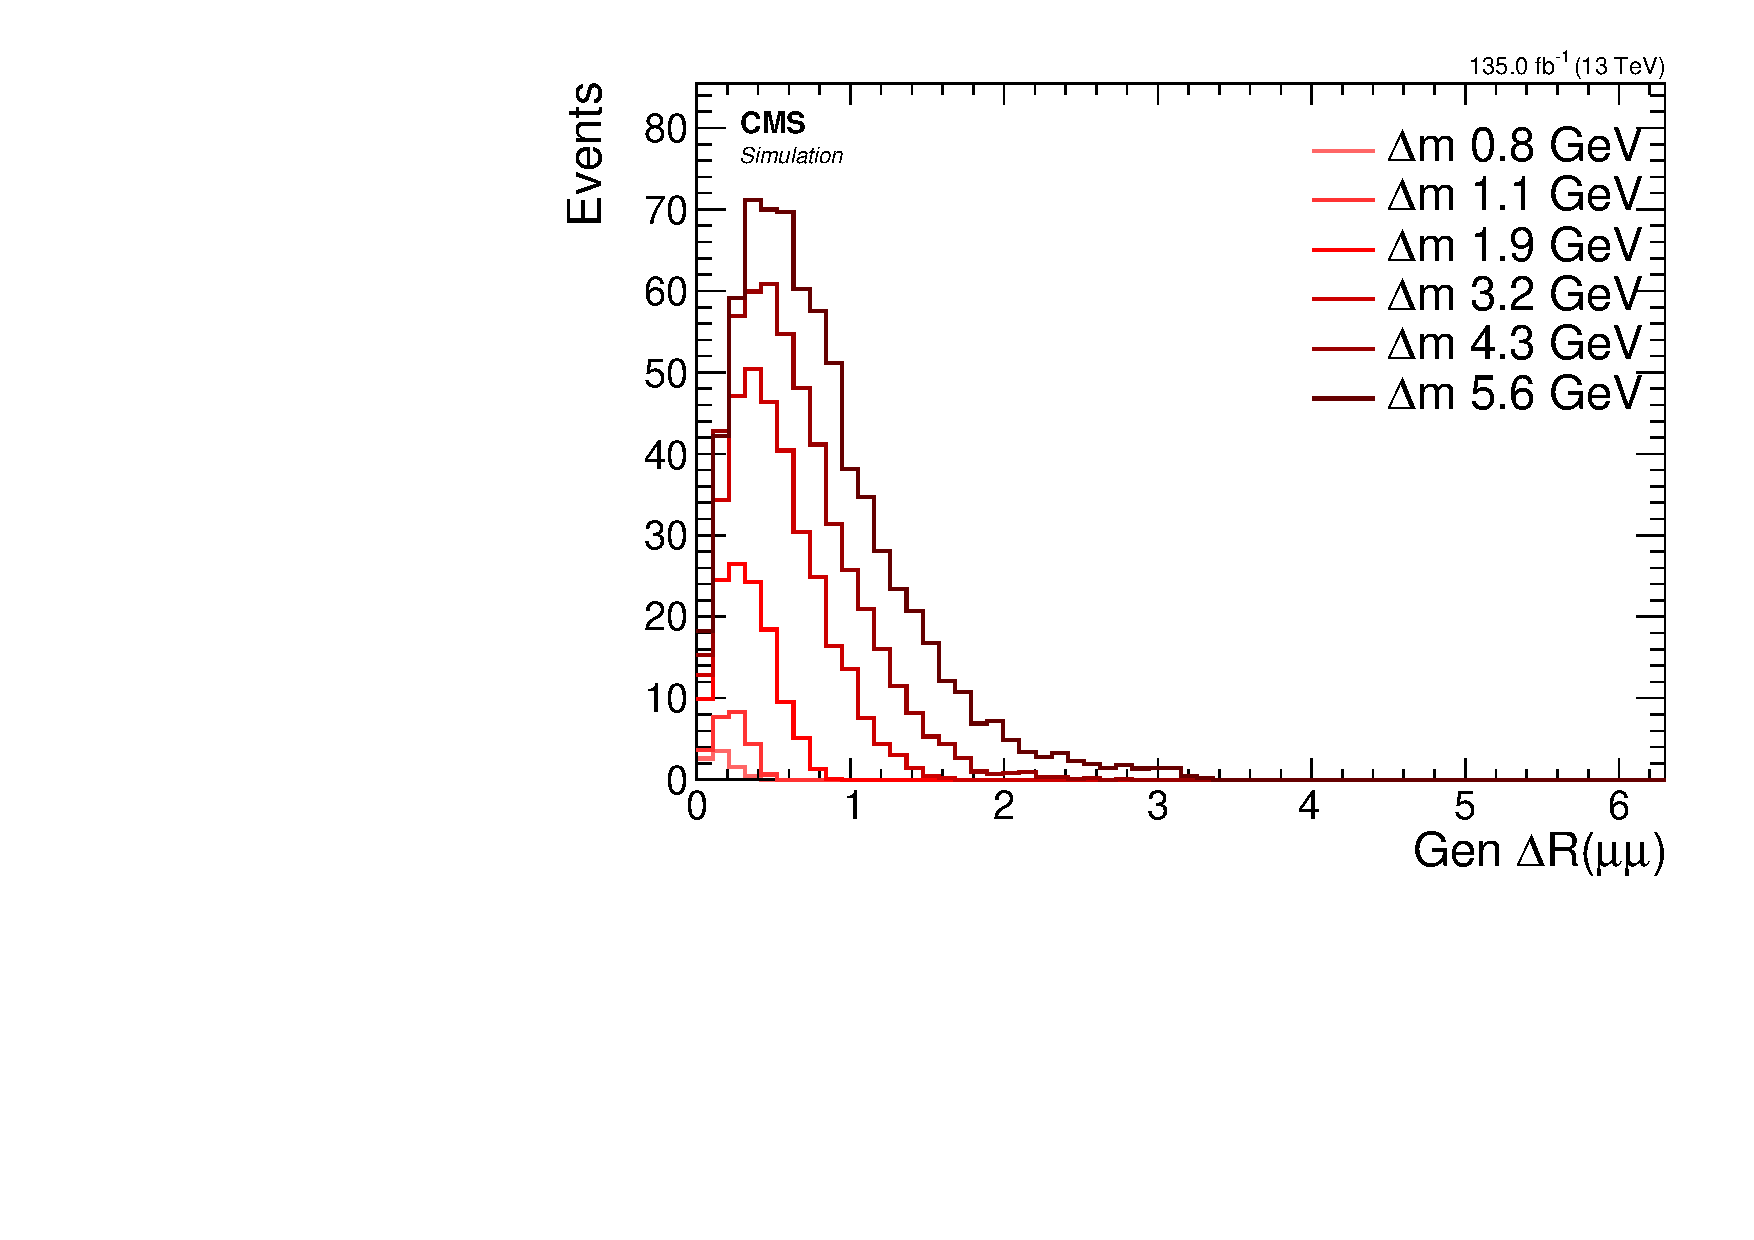
\includegraphics[width=0.32\linewidth]{plots/signal_muons_gen/none_gen_deltaR_cut.pdf}  \,
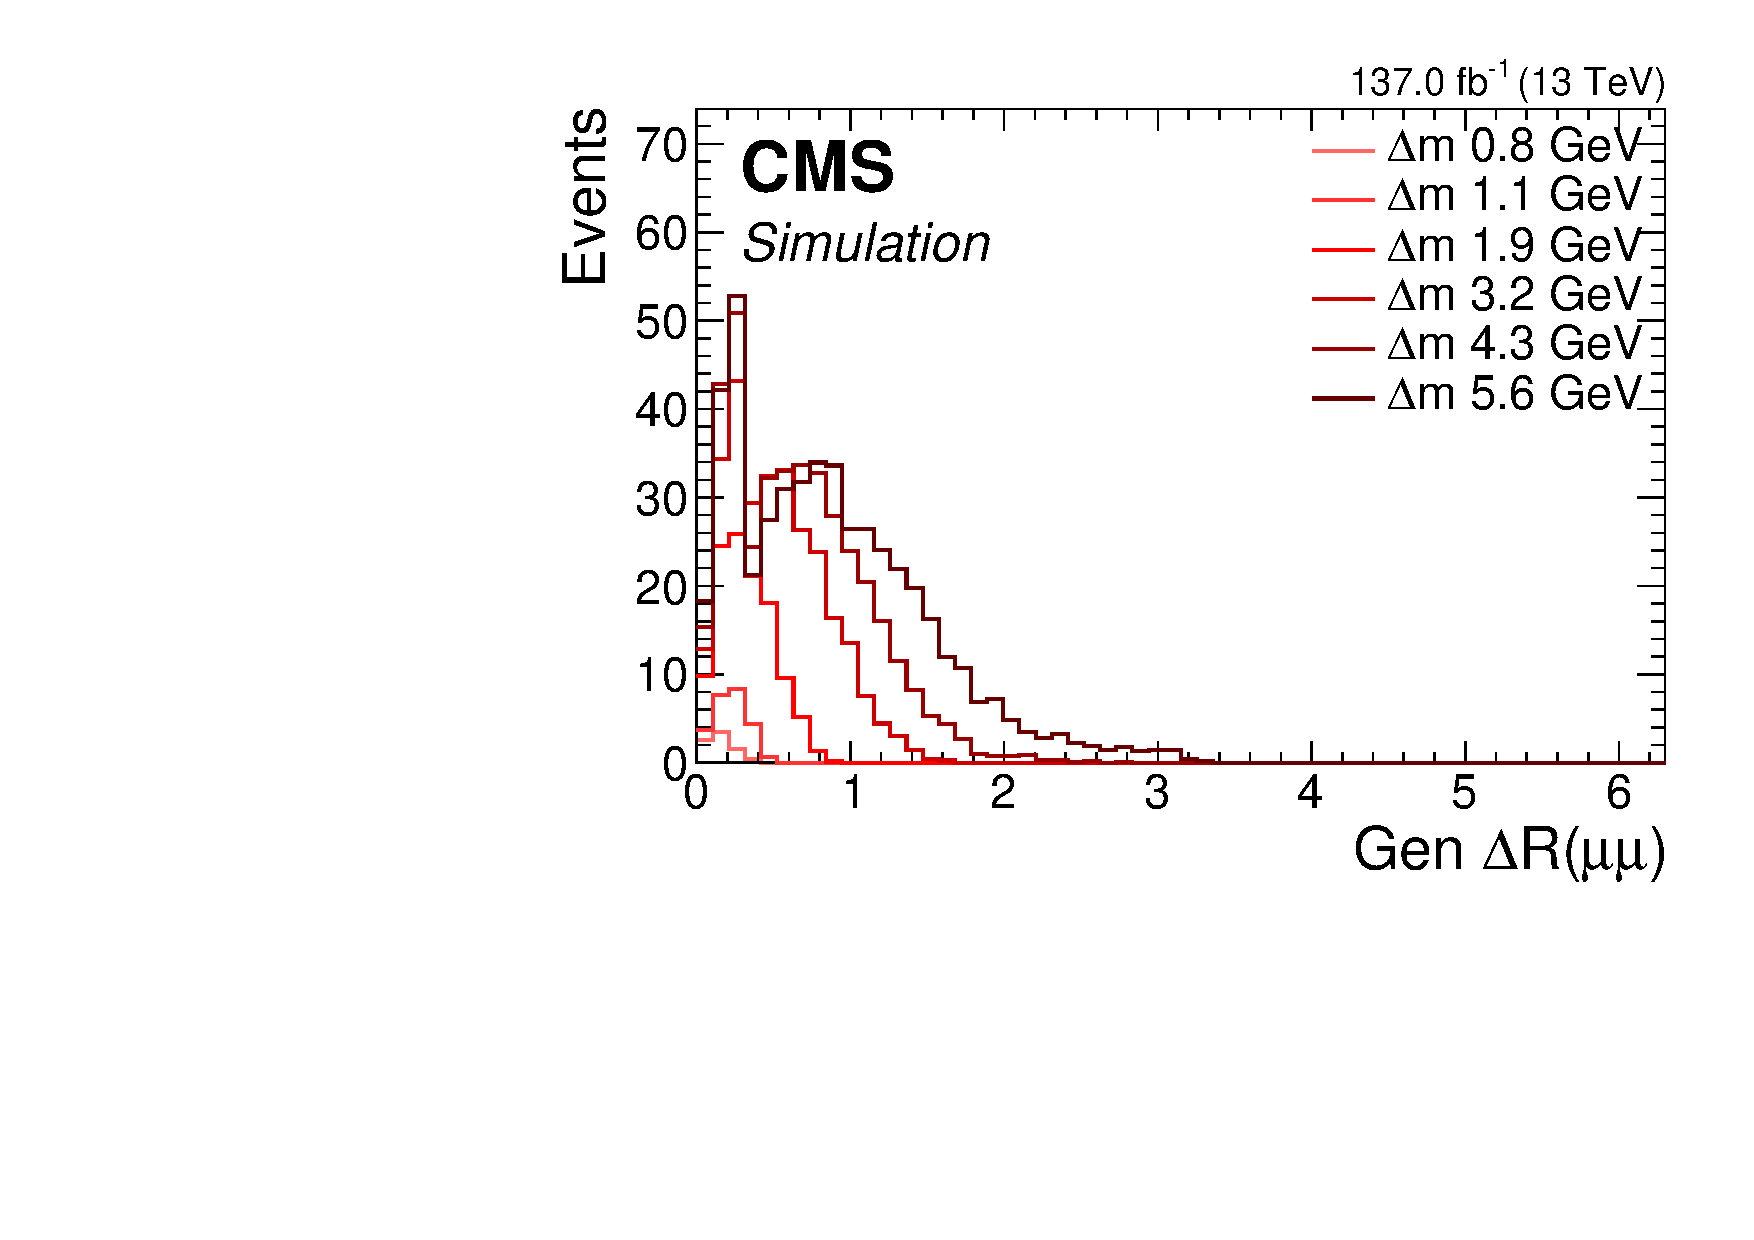
\includegraphics[width=0.32\linewidth]{plots/signal_muons_gen/none_gen_deltaR_orth.pdf} \\
\caption[Signal generator level \DR distributions]{ Signal generator level \gls{dr} distributions with no cuts (left), with $\pt\left(\mu_i\right)>2\GeV,\,i=1,2$ (middle) and with \gls{sos} orthogonality condition $\pt\left(\mu_i\right)>2\GeV$, $\pt\left(\mu_2\right)\leq~3.5\GeV\text{ or }\DR\leq 0.3$ (right).}
\label{fig:signal-generator-dr}
\end{figure}

As can be seen on the left plot, roughly the same amount of events are produced for all \dm model points, but when applying a cut of $\pt\left(\mu\right)>2\GeV$, a hierarchy of \dm points forms, with less events as \dm becomes smaller (middle plot). The spike on the right plot is due to the \gls{sos} orthogonality condition which requires $\drll\leq 0.3$ as one of two conditions in an or statement.
To understand the shaping and hierarchy formation due to the \gls{pt} cut, we repeat the trick from the \mmumu in~\ref{sec:gen-invariant-mass} and plot the \pt of the muons \vs \drll.

\begin{figure}[!htb]
\centering
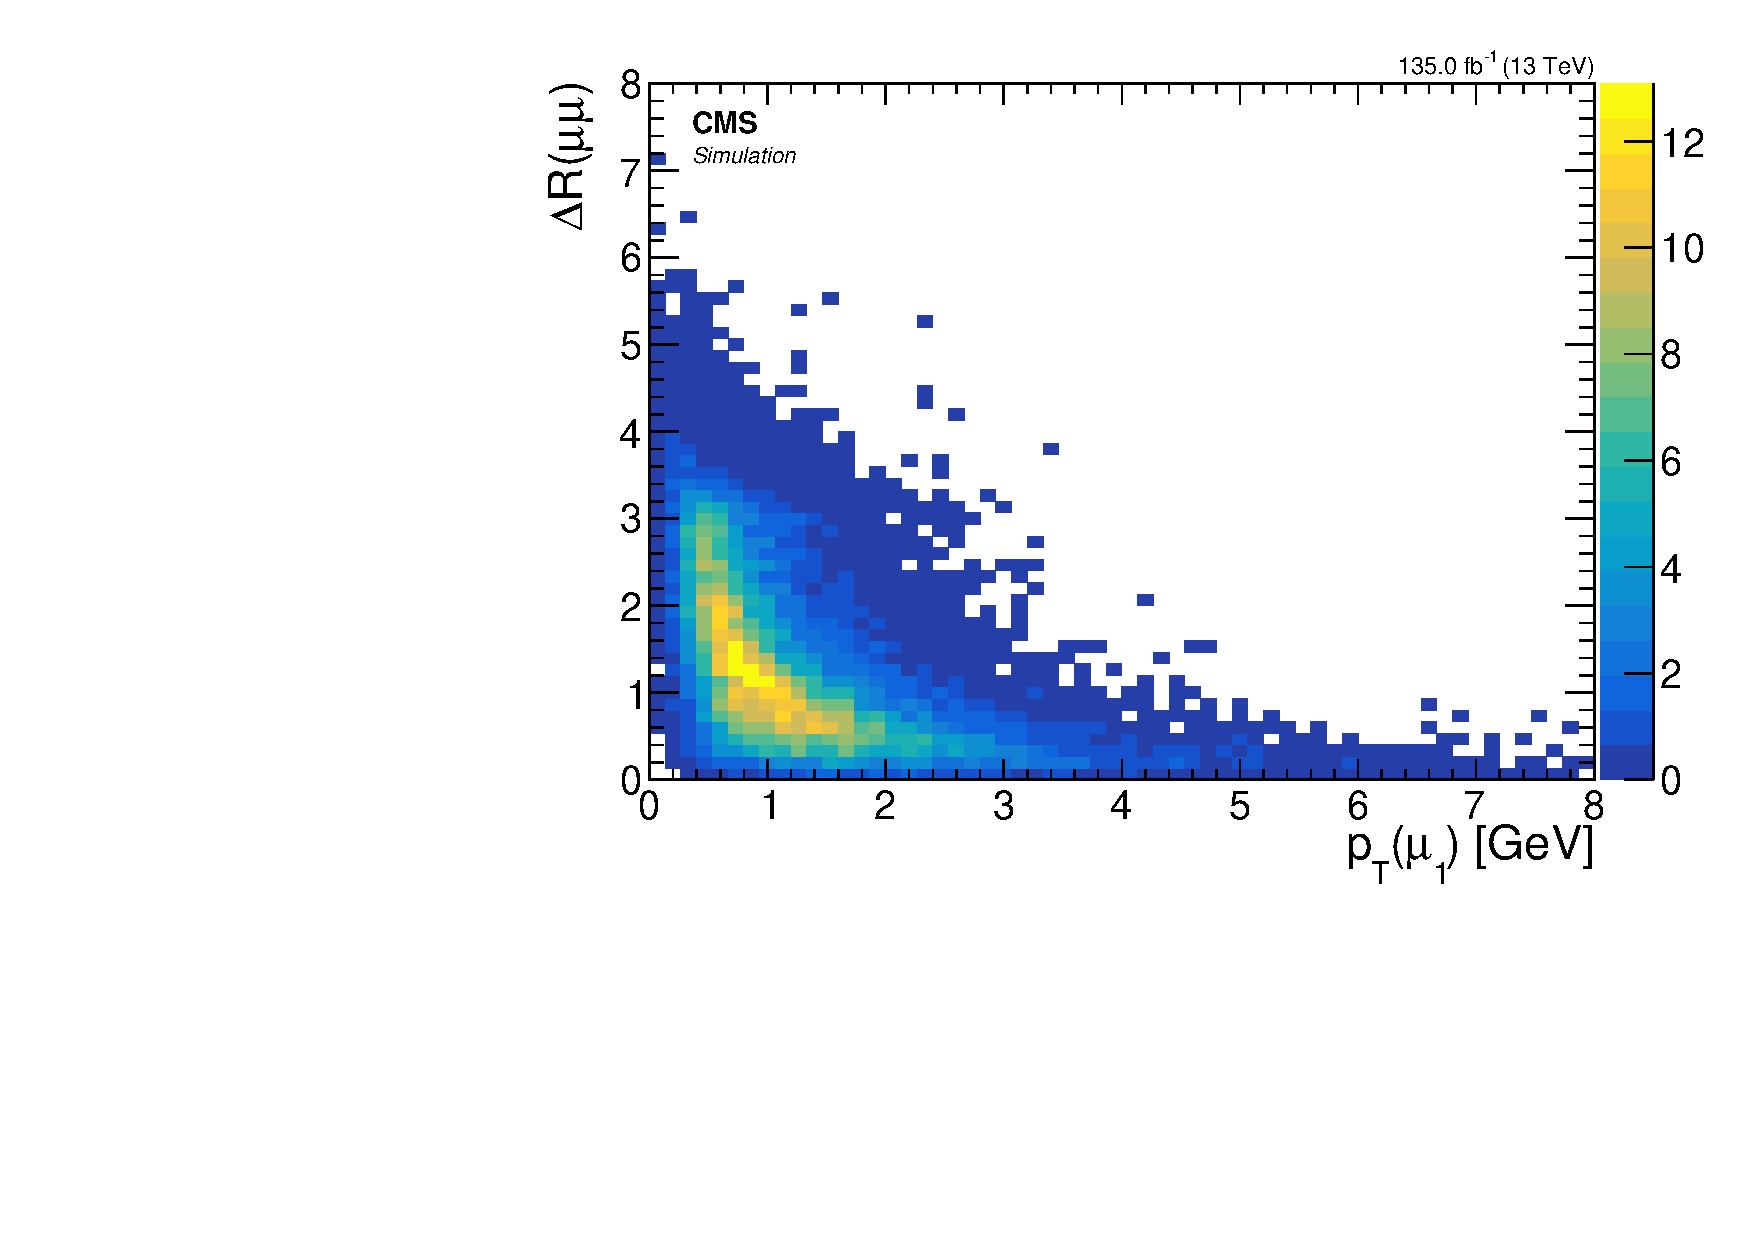
\includegraphics[width=0.48\linewidth]{plots/signal_muons_gen_delta_r_vs_pt/none_gen_delta_r_vs_pt_1.pdf} \,
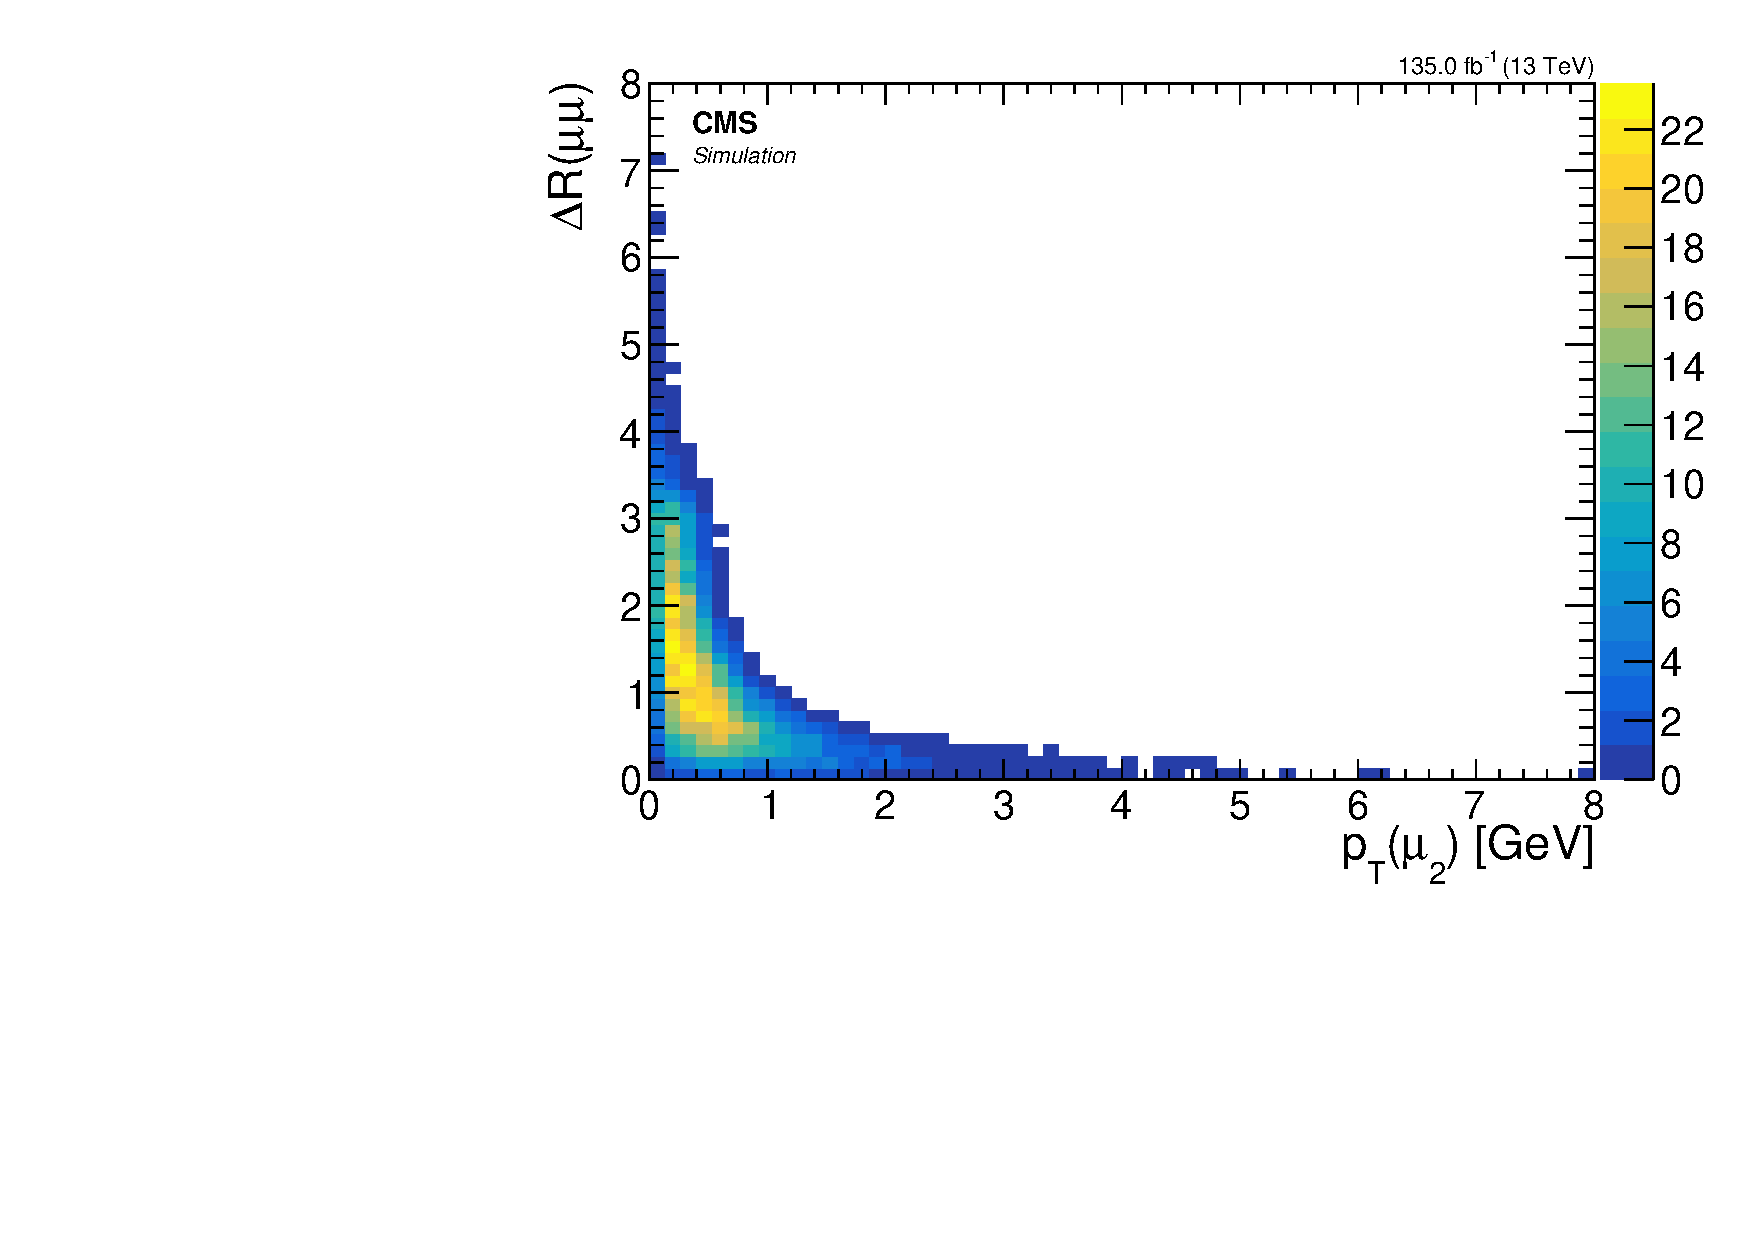
\includegraphics[width=0.48\linewidth]{plots/signal_muons_gen_delta_r_vs_pt/none_gen_delta_r_vs_pt_2.pdf}  \\
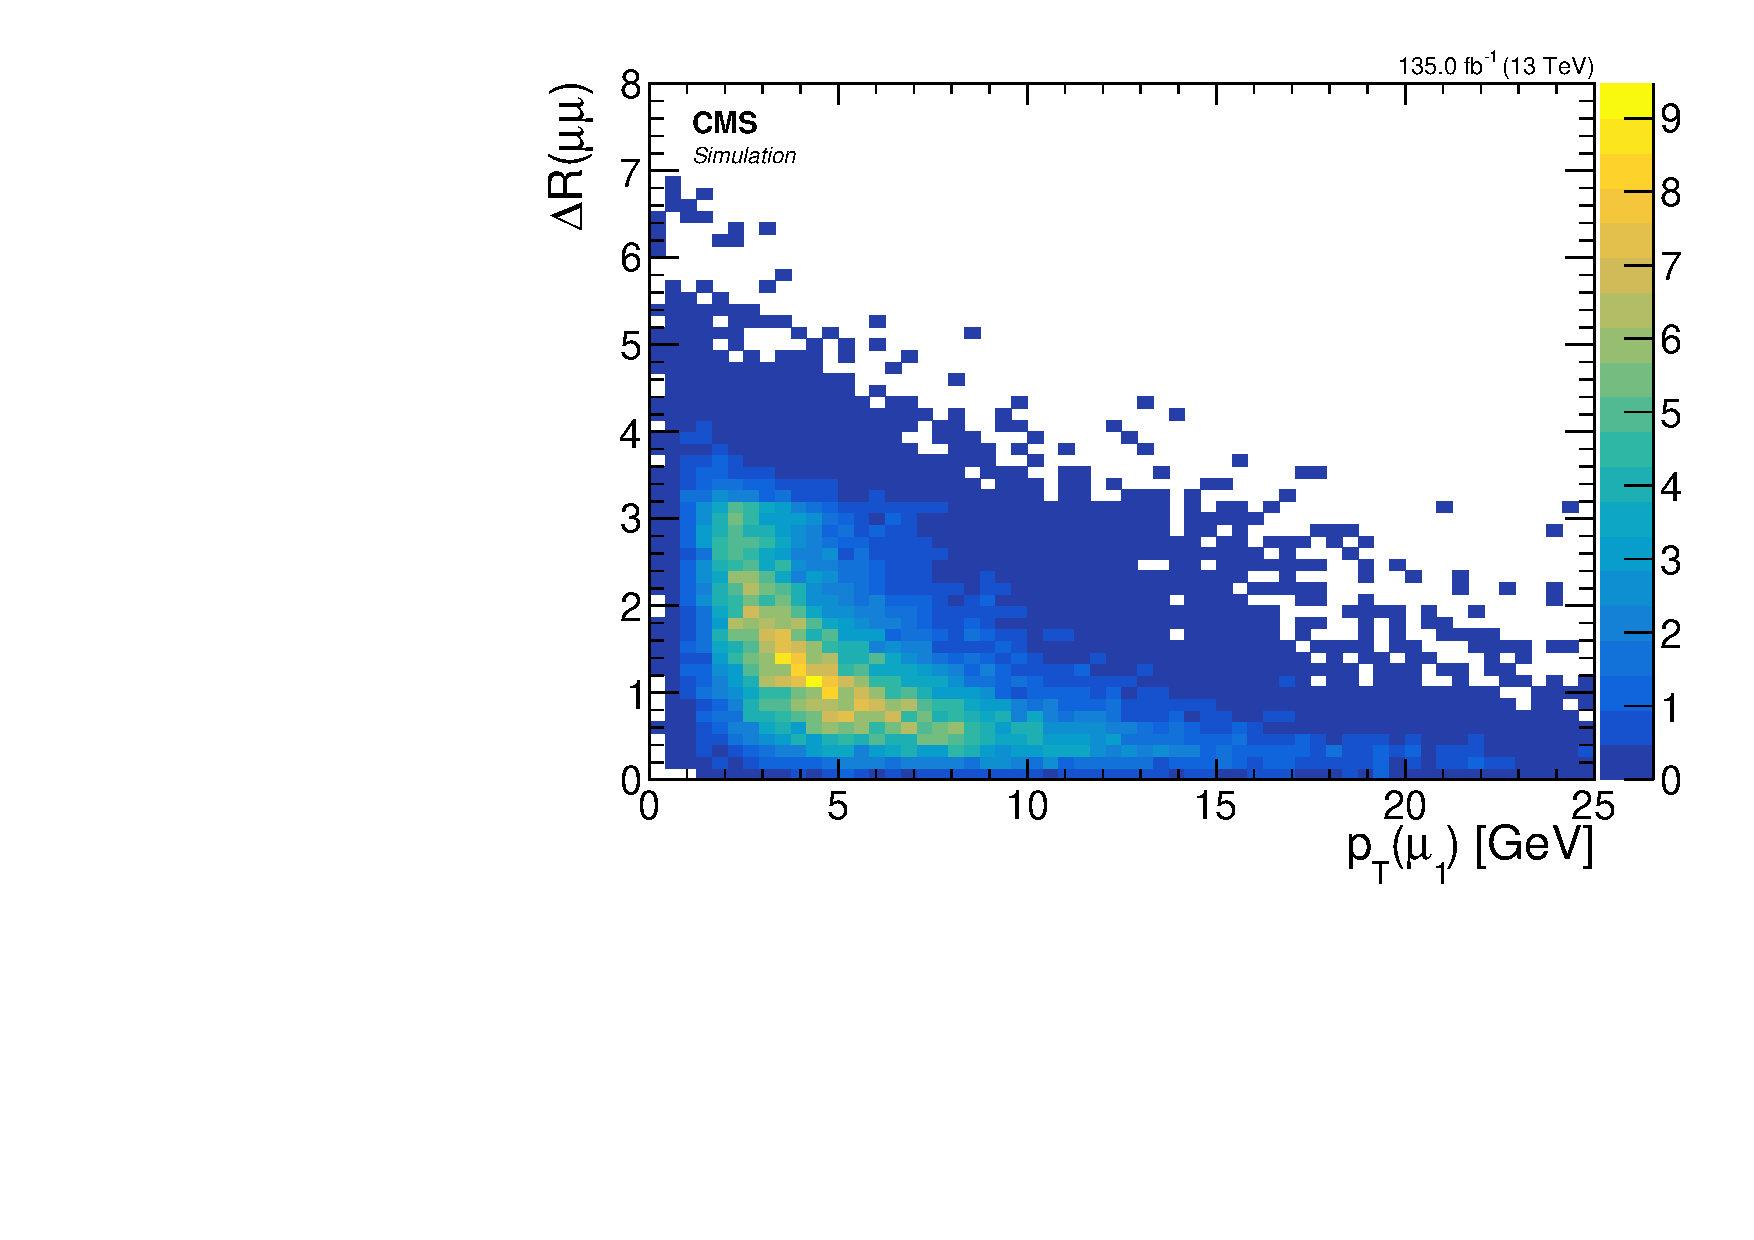
\includegraphics[width=0.48\linewidth]{plots/signal_muons_gen_delta_r_vs_pt_dm5/none_gen_delta_r_vs_pt_1.pdf} \,
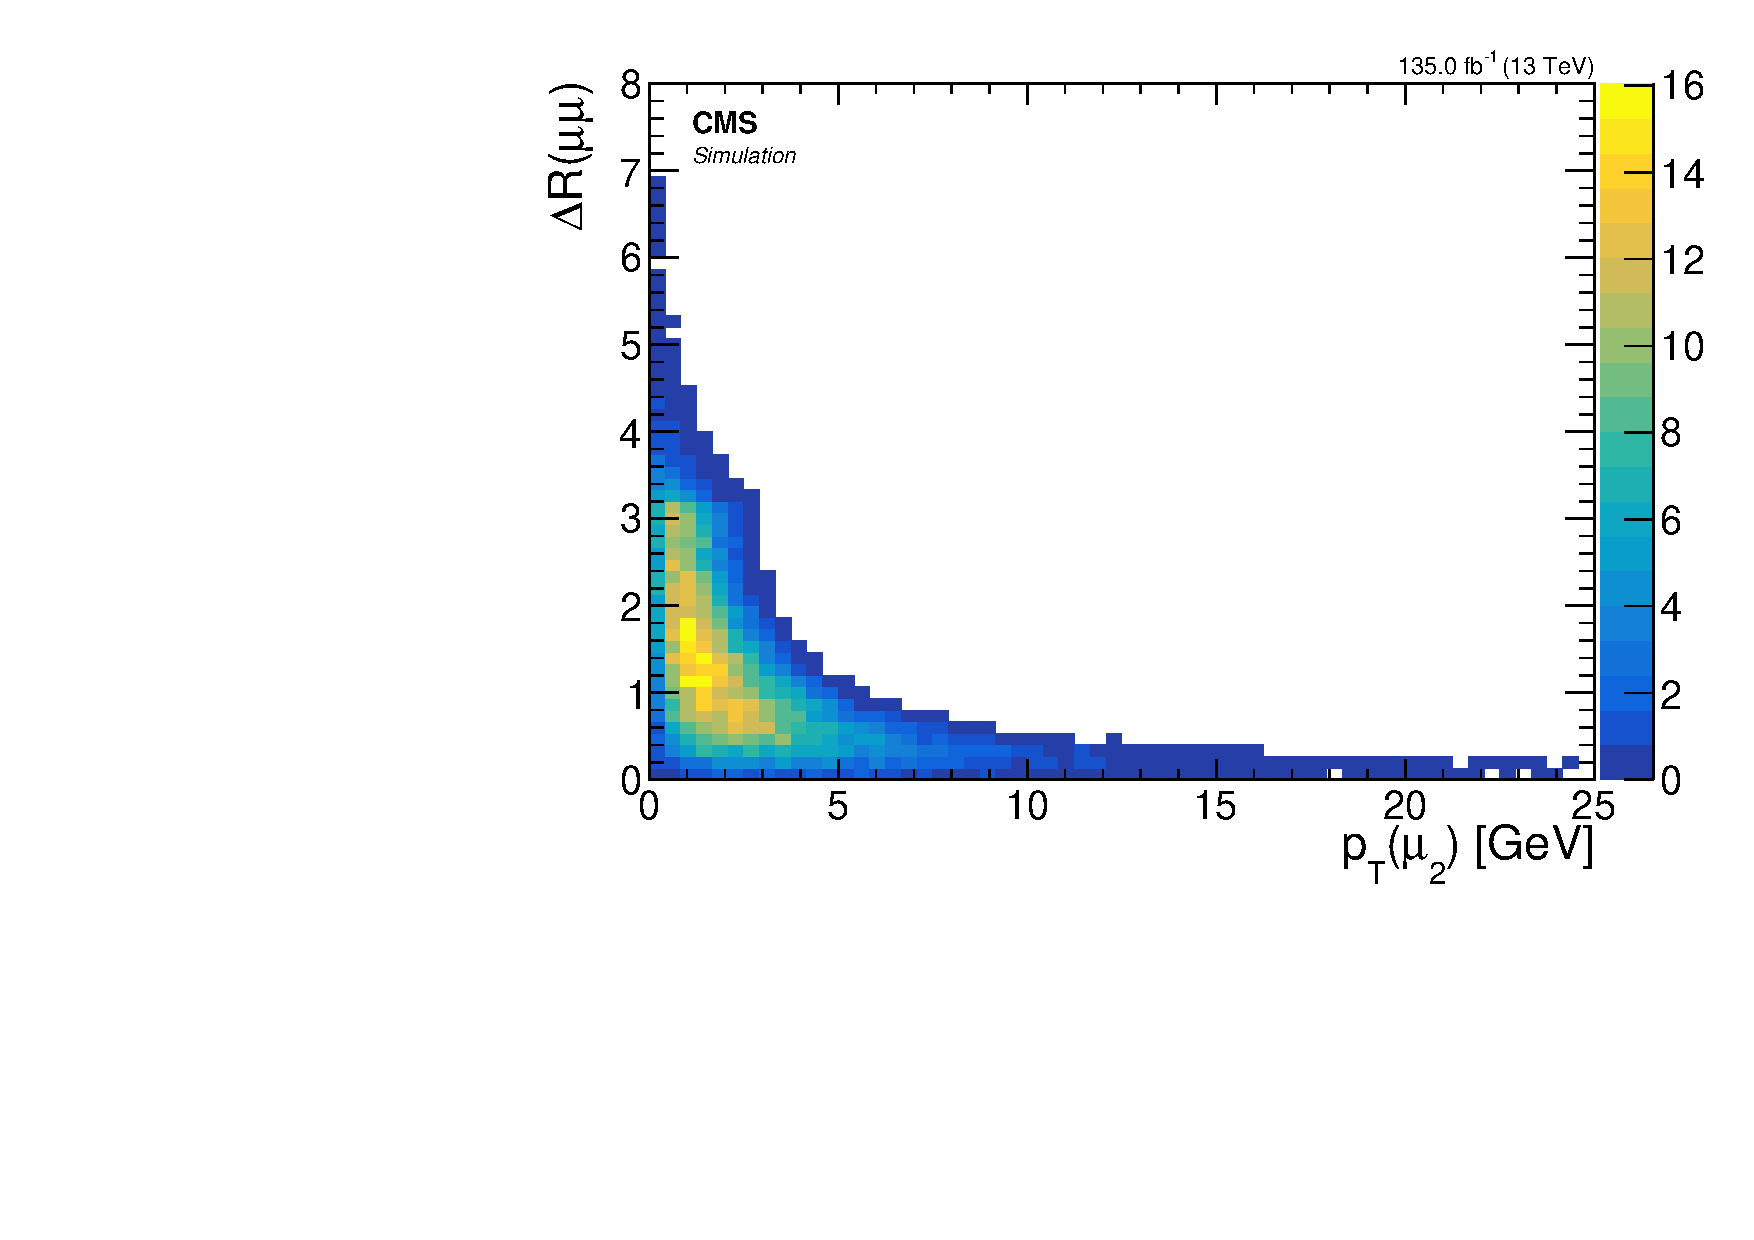
\includegraphics[width=0.48\linewidth]{plots/signal_muons_gen_delta_r_vs_pt_dm5/none_gen_delta_r_vs_pt_2.pdf}  \\
\caption[Signal \drmm \vs \pt]{ Signal \drmm \vs \pt for leading lepton $\mu_1$ (left) and subleading lepton $\mu_2$ (right) for $\dm=1.13\GeV$ (top) and $\dm=5.63\GeV$ (bottom).}
\label{fig:signal-gen-dr-pt}
\end{figure}

Now the hierarchy can be understood by observing that for $\dm=1.13\GeV$, cutting $\pt\left(\mu_2\right)\geq 2\GeV$ will limit the range of \drmm to less than $0.4$ while leaving quite a large range exceeding 3 for the $\dm=5.63\GeV$ model point.

We conclude therefore, that even before taking into consideration reconstruction efficiency of the leptons, to gain access and sensitivity to the low \dm model points, we must be able to probe low \drll values, potentially with values less than 0.3. In the next sections we will need to study reconstructed leptons and define isolation criteria that will enable us to retain signal points with close lepton pairs.

As we have seen for \mmumu in~\ref{sec:gen-invariant-mass}, reconstruction has an effect on both the shape and overall count of events. We look here at those effects on the \drmm distributions.

\begin{figure}[!htb]
\centering
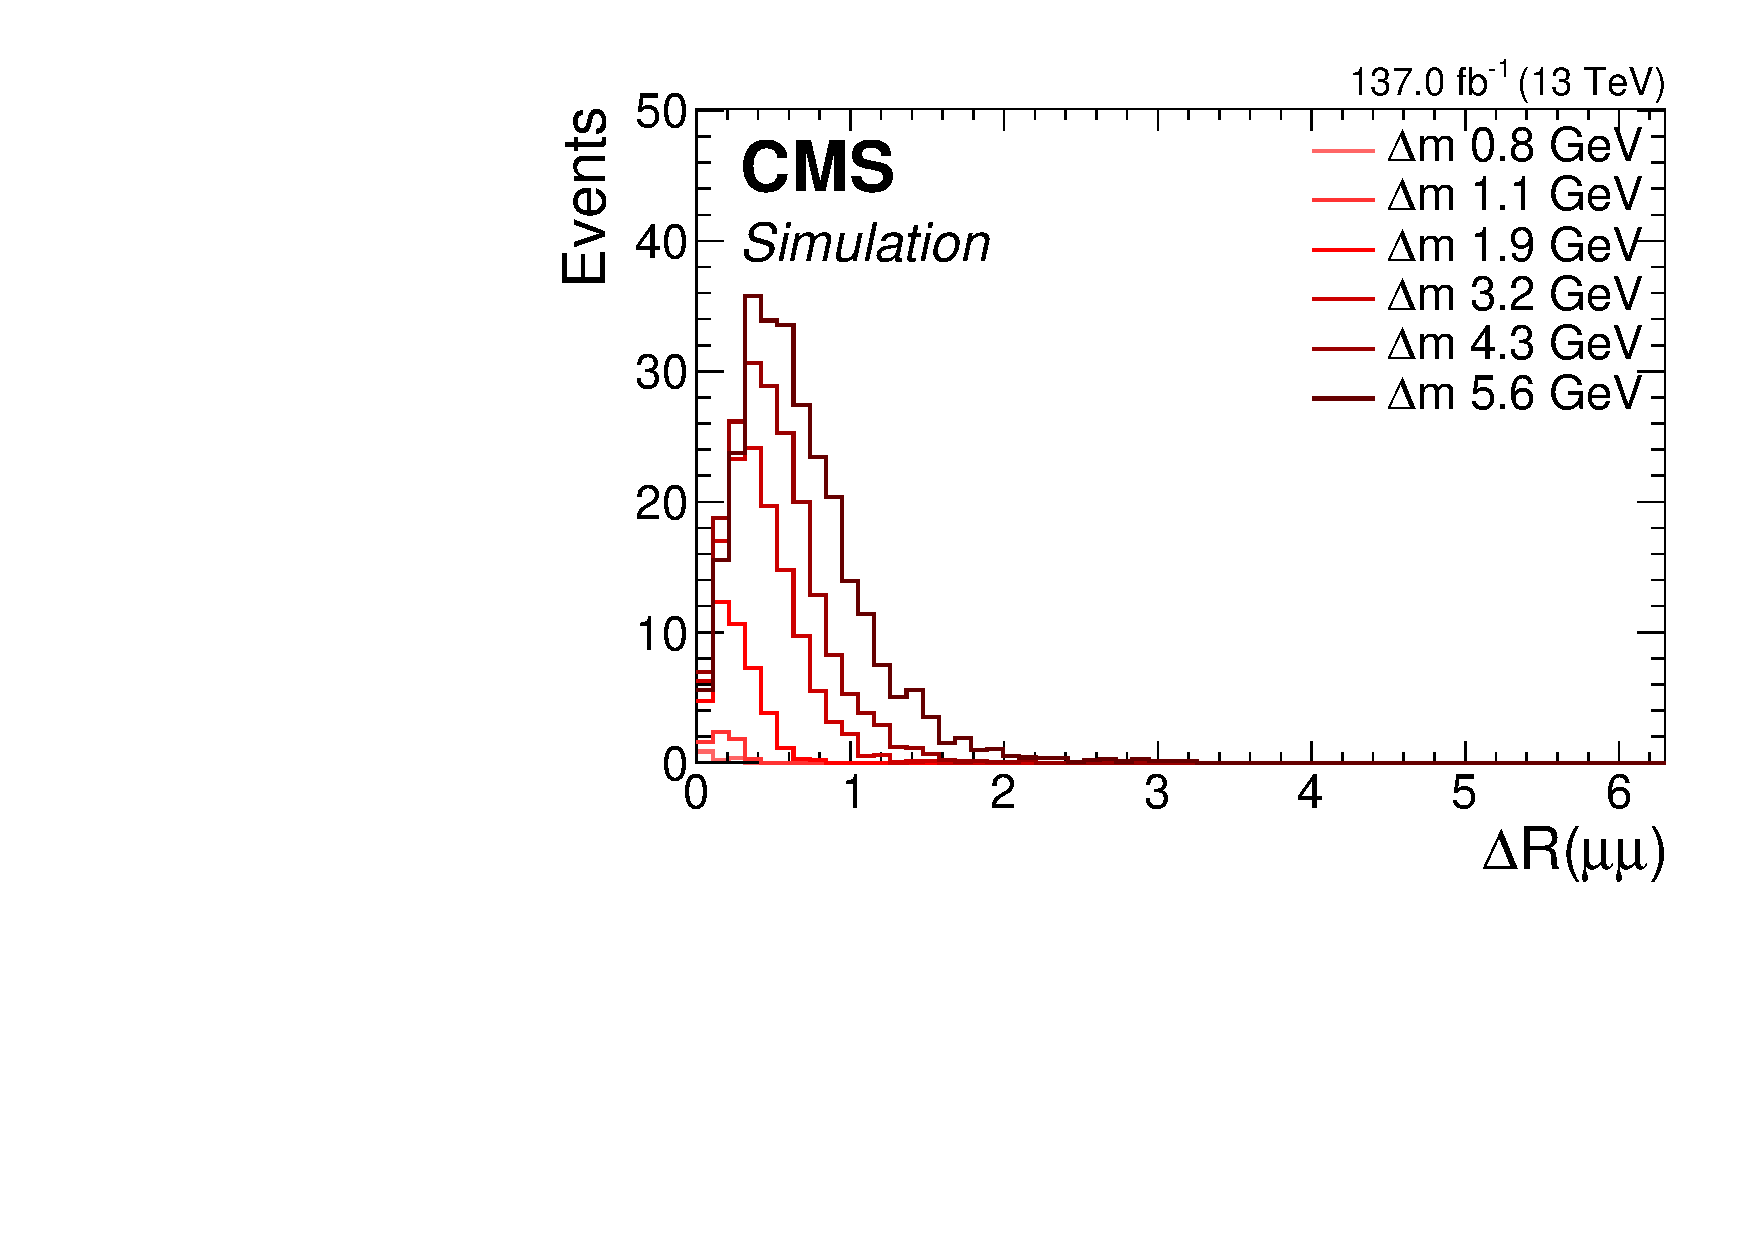
\includegraphics[width=0.48\linewidth]{plots/signal_muons/none_deltaRCorrJetNoMultIso10Dr0.6.pdf} \,
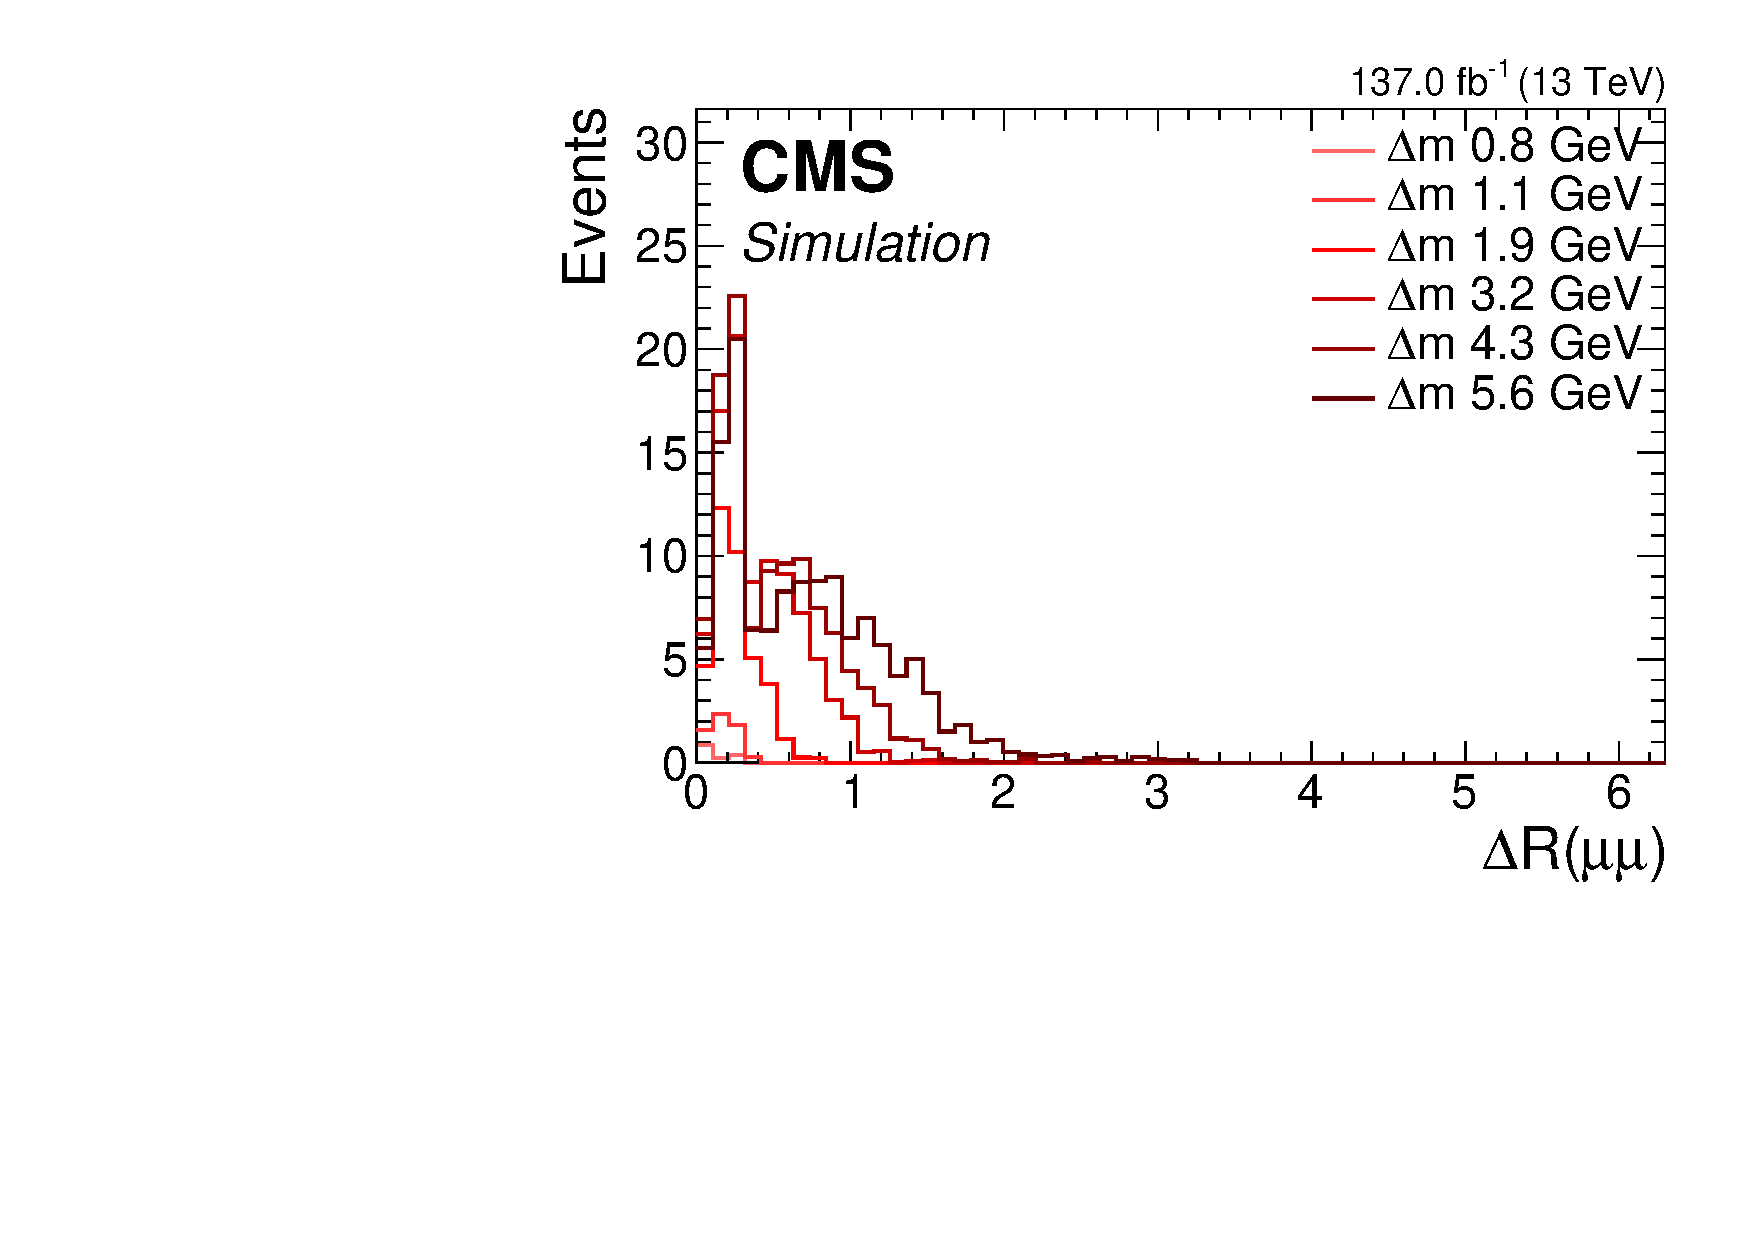
\includegraphics[width=0.48\linewidth]{plots/signal_muons/none_deltaRCorrJetNoMultIso10Dr0.6_orth.pdf}  \\
\caption[Signal reconstructed \drmm]{ Signal reconstructed \drmm with basic analysis selection (left) and additional \gls{sos} orthogonality condition (right).}
\label{fig:reco-signal-dr}
\end{figure}

When we compare the reconstructed \drmm distributions~\ref{fig:reco-signal-dr} to the generator level ones at~\ref{fig:signal-generator-dr} we see that the main effect of the reconstruction on the \drmm is the overall normalization due to reconstruction efficiency.

\subsection{Main drivers of sensitivity}

We attempt to draw conclusion from this signal distribution studies in regards to the main drivers to the sensitivity of different model points of this analysis, as well as of future analysis that might attempt to expend on this one. In this section we have not looked at \gls{sm} background at all. Therefore, it is hard to conclude what effects changing the cuts to \MET or other event level observables might have. However, one thing is very clear from examining the dilepton kinematics and that is that to gain access to low \dm model points, one must lower the threshold on of \pt in the selection of the decay leptons and make sure to also be able to probe low \gls{dr}. Another driver of the sensitivity at all \dm model points is the luminosity, since the production cross section drops as a function of the higgsino mass parameter $\mu$.

We will explore in the next sections how we are able to lower the threshold on the muons transverse momentum as well as dealing with collimated leptons that might pose a challenge. 